\chapter{Wyniki oceny eksperymentalnej}
\label{Section:Results}

\noindent W ramach niniejszego rozdziału zaprezentowane zostaną wyniki oceny eksperymentalnej dokonanej dla 6 algorytmów przetwarzania strumieni danych: \textit{Online Bagging}, \textit{Undersampling Online Bagging}, \textit{Oversampling Online Bagging}, \textit{Neighbourhood Undersampling Online Bagging}, \textit{Neighbourhood Oversampling Online Bagging}, \textit{Hybrid Neighbourhood Online Bagging}.

Ocena eksperymentalna będzie dokonywana na stworzonych przez generator (opisany w rozdziale \ref{Chapter:Generator}) przykładach strumieni danych. Każdy strumień składa się z 200 000 przykładów, gdzie każdy przykład opisany jest przez 5 atrybutów numerycznych oraz etykietę. Jeżeli w strumieniu występuje dryf pojęć to jest to dryf stopniowy (\textit{incremental}), który ma miejsce od momentu przetwarzania przykładu numer 70 000 do momentu przetworzenia przykładu numer 100 000. Dodatkowo każda z klas, przed możliwym wystąpieniem dryfu, jest równoliczna (jeśli nie skorzystano z opcji \textit{StaticIm}) oraz wszystkie przykłady z klasy mniejszościowej oraz większościowej są oznaczone jako typ \textit{Safe}. W ramach dokonanych eksperymentów rozważany jest problem klasyfikacji binarnej.

W pierwszej części tego rozdziału zostanie zaprezentowana ocena algorytmów: \textit{OB}, \textit{UOB}, \textit{OOB}, \textit{NUOB}, \textit{NOOB}. Przeprowadzona ocena będzie składała się z kilku sekcji: analiza na strumieniach z jednym czynnikiem trudności (\english{single factors}), analiza na strumieniach z dwoma czynnikami trudności (\english{pairs of factors}) oraz analiza na złożonych strumieniach zawierających wiele czynników trudności (\english{complex scenarios}). W identyczny sposób będzie przebiegała druga częśc tego rozdziału, gdzie zostanie zaprezentowana ocena algorytmów: \textit{UOB}, \textit{OOB}, \textit{NUOB}, \textit{NOOB}, \textit{HNOB}.

Ocena klasyfikatorów będzie przebiegała na podstawie wykorzystania dwóch miar: czułości (\english{recall}) oraz \textit{G-mean}. Miara czułości w tym przypadku odpowiedzialna jest za sprawdzanie jakości klasyfikacji przykładów z klasy mniejszościowej. Miara \textit{G-mean} z kolei pozwala na sprawdzanie jakości klasyfikacji przykładów z obu badanych klas. Poprzez równoczesną analizę obu tych miar jest możliwe zaobserwowanie sytuacji, w których jakość klasyfikacji przykładów jednej z klas zaczyna spadać. Przykładowo jeżeli wartość miary \textit{Recall} zacznie wzrastać i w tym samym czasie wartość miary \textit{G-mean} zacznie maleć to oznacza, że jakość klasyfikacji przykładów z klasy mniejszościowej wzrasta, ale kosztem poprawnego rozpoznawania przykładów z klasy większościowej. Dodatkowym atutem miary \textit{G-mean} jest fakt, że interpretacja tej miary pozostaje taka sama dla wszystkich możliwych wartości współczynników niezbalansowania klas (\english{imbalance ratios}), co jest szczególnie istotne przy badaniu zmiennych współczynników niezbalansowania \cite{Article:TypyPrzykladow}.

Zarówno miara \textit{Recall} jak i \textit{G-mean} zostały obliczone przy wykorzystaniu okna przesuwnego zawierającego liczbę 1000 ostatnich przykładów \cite{Article:Evaluation}. Każdy przeanalizowany strumień danych został zwizualizowany przy wykorzystaniu wykresu liniowego z liczbą przetworzonych przykładów na osi X, wartością miary \textit{Recall}/\textit{G-mean} na osi Y oraz zaznaczonym, poprzez szare tło, regionem dryfu pojęć. Przedstawiane wykresy liniowe zostały wygładzone przy wykorzystaniu mechanizmu średniej ruchomej składającej się z 20 punktów \cite{Article:TypyPrzykladow}.

Dodatkowo odnotowane wartości miar zostały uśrednione dla badanych strumieni danych, co stanowiło podstawę do przeprowadzenia testu statystycznego rang Friedman'a \cite{Article:Friedman}, którego celem było porównanie jakości klasyfikacji badanych klasyfikatorów \cite{Article:TypyPrzykladow}. Ze względu na zbyt dużą liczbę przeprowadzonych eksperymentów, w rozdziale tym zawarte zostały tylko najbardziej reprezentatywne wykresy. Pozostałe wyniki, które nie zostały przedstawione w niniejszej rozprawie, są dostępne do wglądu w repozytorium, dostępnym jako załącznik \ref{Chapter:Repository} do rozprawy.

Organizacja oraz struktura prezentacji wyników oceny eksperymentalnej jest inspirowana pracą \cite{Article:TypyPrzykladow}. Zaprezentowane w tym rozdziale algorytmy zostały zaimplementowane w języku \textit{Java} przy pomocy biblioteki \textit{Massive Online Analysis (MOA)} \cite{Article:MOA}. W przypadku algorytmów \textit{OOB} oraz \textit{UOB} skorzystano z implementacji autorstwa Leandro L. Minku dostępnej na platformie \textit{GitHub}\footnote{\url{https://github.com/minkull/UOB-OOB-MultiClass}}. Wszelakie skrypty, konieczne do wygenerowania wykresów wykorzystanych w niniejszej rozprawie, pochodzą z ogólnodostępnego repozytorium \textit{GitHub}\footnote{\url{https://github.com/dabrze/imbalanced-stream-generator}} Dariusza Brzezińskiego.

\section{Porównanie istniejących algorytmów z nowymi propozycjami}
\label{Section:AlgorithmsComparison}

\noindent W ramach wykonanych testów każdy z przetestowanych algorytmów charakteryzował się następującymi wartościami parametrów:

\begin{itemize}
    \item liczba klasyfikatorów składowych - 15
    \item rodzaj klasyfikatora składowego - drzewo Hoeffding'a (ze standardowymi wartościami parametrów)
\end{itemize}

\noindent W tym przypadku wartości dla tych parametrów zostały dobrane zgodnie wartościami wykorzystanymi w pracy \cite{Article:TypyPrzykladow}. Algorytmy \textit{UOB} oraz \textit{OOB} wykorzystywały dodatkowy parametr charakteryzujący się następującą wartością:

\begin{itemize}
    \item współczynnik zapominania ($\theta$) - 0.9
\end{itemize}

\noindent Dla parametru współczynnika zapominania wartość 0.9 jest wartością domyślną oraz sugerowaną przez autorów pracy \cite{Article:OBSecond}. Dodatkowymi parametrami, które zostały zawarte w algorytmach \textit{NUOB} oraz \textit{NOOB} były:

\begin{itemize}
    \item liczba najbliższych sąsiadów ($k$) - 5
    \item wielkość okna przesuwnego - 500
    \item dodatkowy współczynnik do obliczania poziomu bezpieczeństwa ($\Psi$) - 2.0
\end{itemize}

\noindent W przypadku wyboru wartości parametrów dla liczby najbliższych sąsiadów zdecydowano się posłużyć eksperymentami wykonanymi przez autorów pracy \cite{Article:NNBag}. W ramach swojej pracy przetestowali różne wartości parametrów dla $k$ = 5, 7, 9 i 11. Końcowym wynikiem oceny eksperymentalnej był wniosek dotyczący tego, że dobre rezultaty jakości klasyfikacji można osiągnąć dla małych wartości parametru $k$ zarówno dla \textit{undersampling'u} jak i \textit{oversampling'u}. Dla parametrów dotyczących wielkości okna przesuwnego oraz dodatkowego współczynnika do obliczania poziomu bezpieczeństwa zdecydowano się przeprowadzić dodatkowe testy na wybranych strumieniach danych.

Dla parametru dotyczącego wielkości okna przesuwnego przetestowano wartości $500$ oraz $1000$. W ramach wykonanego eksperymentu przetestowano wiele scenariuszy, jednak ze względu na długość pracy, zostaną zaprezentowane jedynie trzy przykładowe scenariusze w celach wizualizacji. Wyniki dotyczące jakości klasyfikacji na wybranych strumieniach danych można zobaczyć na rysunku \ref{Figure:WindowParametrization1} i \ref{Figure:WindowParametrization2}.

\begin{figure}[h]
    \centering
    \subfloat{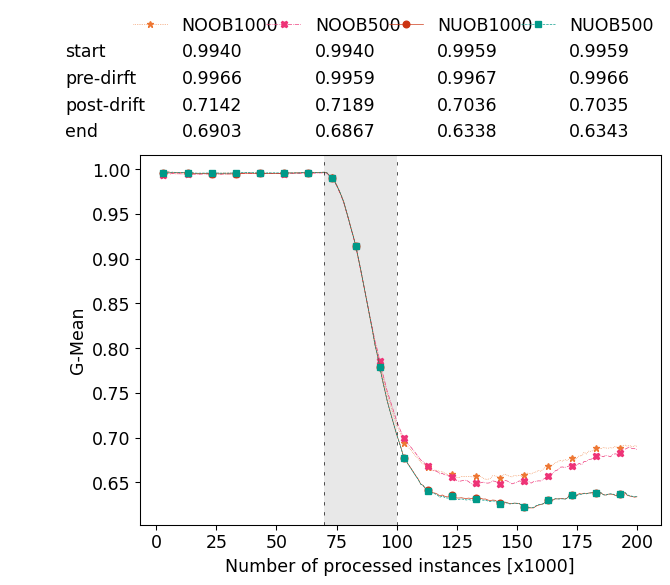
\includegraphics[width=7cm]{figures/rare60_window.png}}
    \qquad
    \subfloat{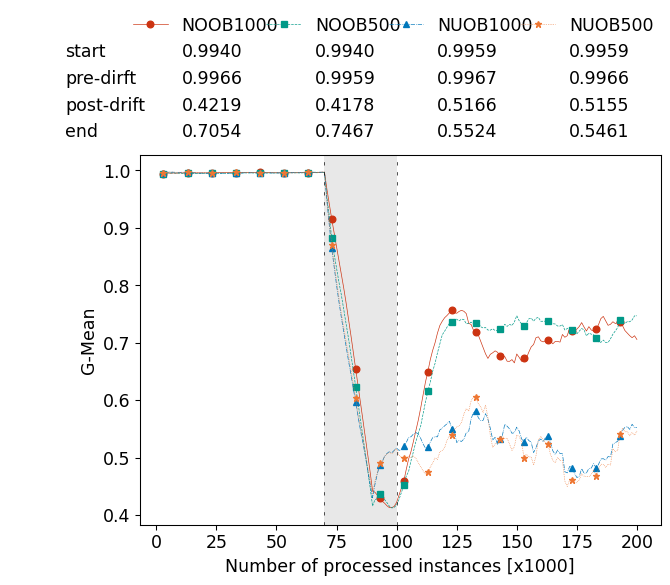
\includegraphics[width=7cm]{figures/im1rare100_window.png}}
    \caption{Wykresy liniowe miary \textit{G-mean} dla strumieni \textit{Rare60} (po lewej) oraz \textit{Im1+Rare100} (po prawej). Liczba zawarta w nazwie algorytmu oznacza wielkość okna przesuwnego}\label{Figure:WindowParametrization1}
\end{figure}

\newpage

\begin{figure}[h]
    \centering
    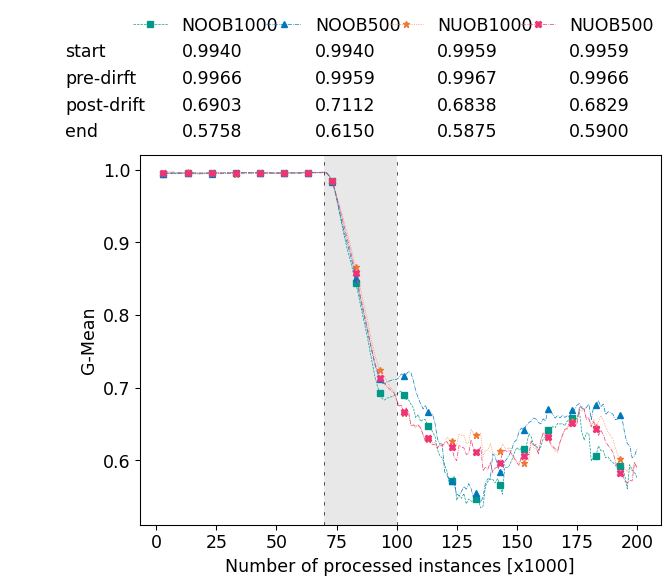
\includegraphics[width=10cm]{figures/split5im1borderline40rare40_window.png}
    \caption{Wykres liniowy miary \textit{G-mean} dla strumienia \textit{Split5+Im1+Borderline40+Rare40}. Liczba zawarta w nazwie algorytmu oznacza wielkość okna przesuwnego}\label{Figure:WindowParametrization2}
\end{figure}


\noindent Jak można zaobserwować na zaprezentowanych rysunkach różnice w jakości klasyfikacji dla zaproponowanych algorytmów są niewielkie między wartością 500 a 1000 dla parametru wielkości okna przesuwnego. Z tego powodu dalsze eksperymenty zdecydowano się przeprowadzić dla wartości parametru równej 500.

Podobna analiza została przeprowadzona dla parametru dotyczącego współczynnika wymagane do obliczania poziomu bezpieczeństwa. W ramach analizy przetestowano wartości $1.5$ oraz $2$. Wyniki dotyczące jakości klasyfikacji na wybranych strumieniach danych można zobaczyć na rysunku \ref{Figure:PsiParametrization1} i \ref{Figure:PsiParametrization2}.

\begin{figure}[h]
    \centering
    \subfloat{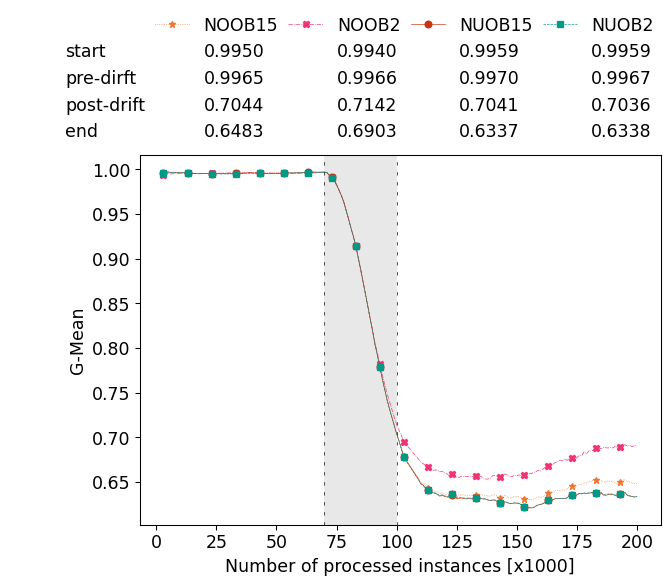
\includegraphics[width=7cm]{figures/rare60_psi.png}}
    \qquad
    \subfloat{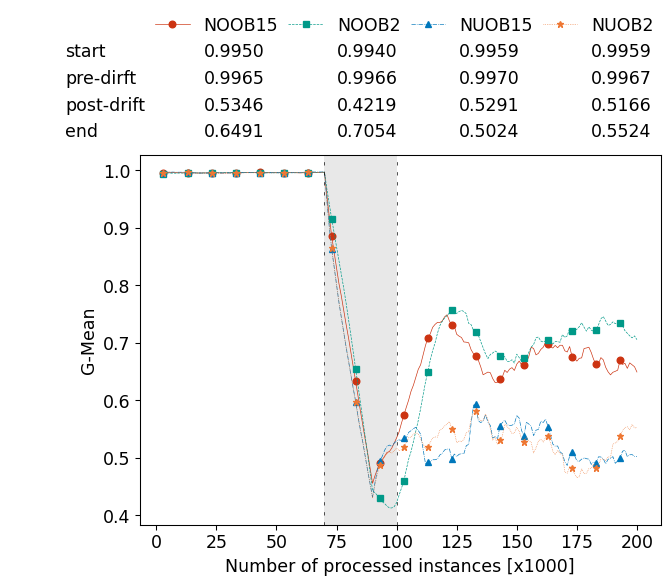
\includegraphics[width=7cm]{figures/im1rare100_psi.png}}
    \caption{Wykresy liniowe miary \textit{G-mean} dla strumieni \textit{Rare60} (po lewej) oraz \textit{Im1+Rare100} (po prawej). Liczba zawarta w nazwie algorytmu oznacza wartość współczynnika (liczba 15 oznacza wartość równą 1.5)}\label{Figure:PsiParametrization1}
\end{figure}

\newpage

\begin{figure}[h]
    \centering
    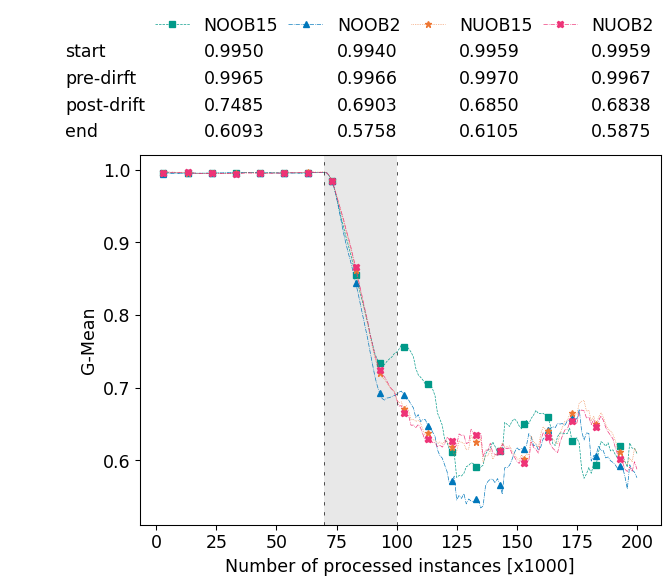
\includegraphics[width=10cm]{figures/split5im1borderline40rare40_psi.png}
    \caption{Wykres liniowy miary \textit{G-mean} dla strumienia \textit{Split5+Im1+Borderline40+Rare40}. Liczba zawarta w nazwie algorytmu oznacza wartość współczynnika (liczba 15 oznacza wartość równą 1.5)}\label{Figure:PsiParametrization2}
\end{figure}

\noindent Na zaprezentowanych pierwszych dwóch wykresach można zaobserwować lekką przewagę w trafności klasyfikacji dla algorytmów wykorzystujących parametr $\Psi$ o wartości równej 2. W przypadku ostatniego scenariusza sytuacja ulega odwróceniu, co sugeruje, że osiągnięcie najlepszego rezultatu tak naprawdę zależy od rodzaju strumienia. W dalszej analizie zdecydowano się wykorzystać wartość parametru równą 2.

\newpage

\subsection{Data streams with single factors}

\noindent W pierwszej kolejności zaprezentowane algorytmy zostaną przetestowane pod kątem jakości klasyfikacji na strumieniach danych z jednym czynnikiem trudności (\english{single factor}).\\\\
\textbf{Stały współczynnik niezbalansowania}\\

\noindent Pierwszym z badanych czynników będzie stały współczynnik niezbalansowania (\textit{StaticIm}). Praktycznie wszystkie algorytmy radziły sobie bardzo dobrze z klasyfikacją danych pochodzących ze strumieni o stałym współczynniku niezbalansowania. Dla strumieni danych o współczynniku niezbalansowania równym: 50\%, 40\%, 30\%, 20\%, 10\% wszystkie algorytmy charakteryzowały się średnią wartością miar \textit{G-mean} oraz \textit{Recall} na poziomie 0.99. Sytuacja trochę zmieniała się dla wartości współczynnika $\leq$ 5\%, gdzie można zauważyć lekki spadek jakości klasyfikacji dla algorytmów \textit{OB}, \textit{OOB} oraz \textit{NOOB}. Wraz ze spadkiem współczynnika niezbalansowania spadała jakość klasyfikacji dla wspomnianych algorytmów - dla współczynnika równego 1\% średnia wartość miary \textit{G-mean} dla algorytmu \textit{OB} wyniosła 0.81, dla algorytmu \textit{NOOB} 0.92, dla algorytmu \textit{OOB} 0.94. Jakość klasyfikacji pozostała niezmienna dla algorytmów \textit{UOB} oraz \textit{NUOB} dla różnych wartości współczynnika niezbalansowania. Szczegółowe wyniki jakości klasyfikacji zostały przedstawione na rysunku \ref{Figure:StaticImbalance} oraz w tabeli \ref{Tab:ImbalanceRatio}. Wartości miar oznaczonych na wykresie oraz zawartych w tabeli zostały wyznaczone jako średnia wszystkich wartości obliczonych podczas ewaluacji odpowiedniego strumienia.\\\\

\begin{figure}[h]
    \centering
    \subfloat{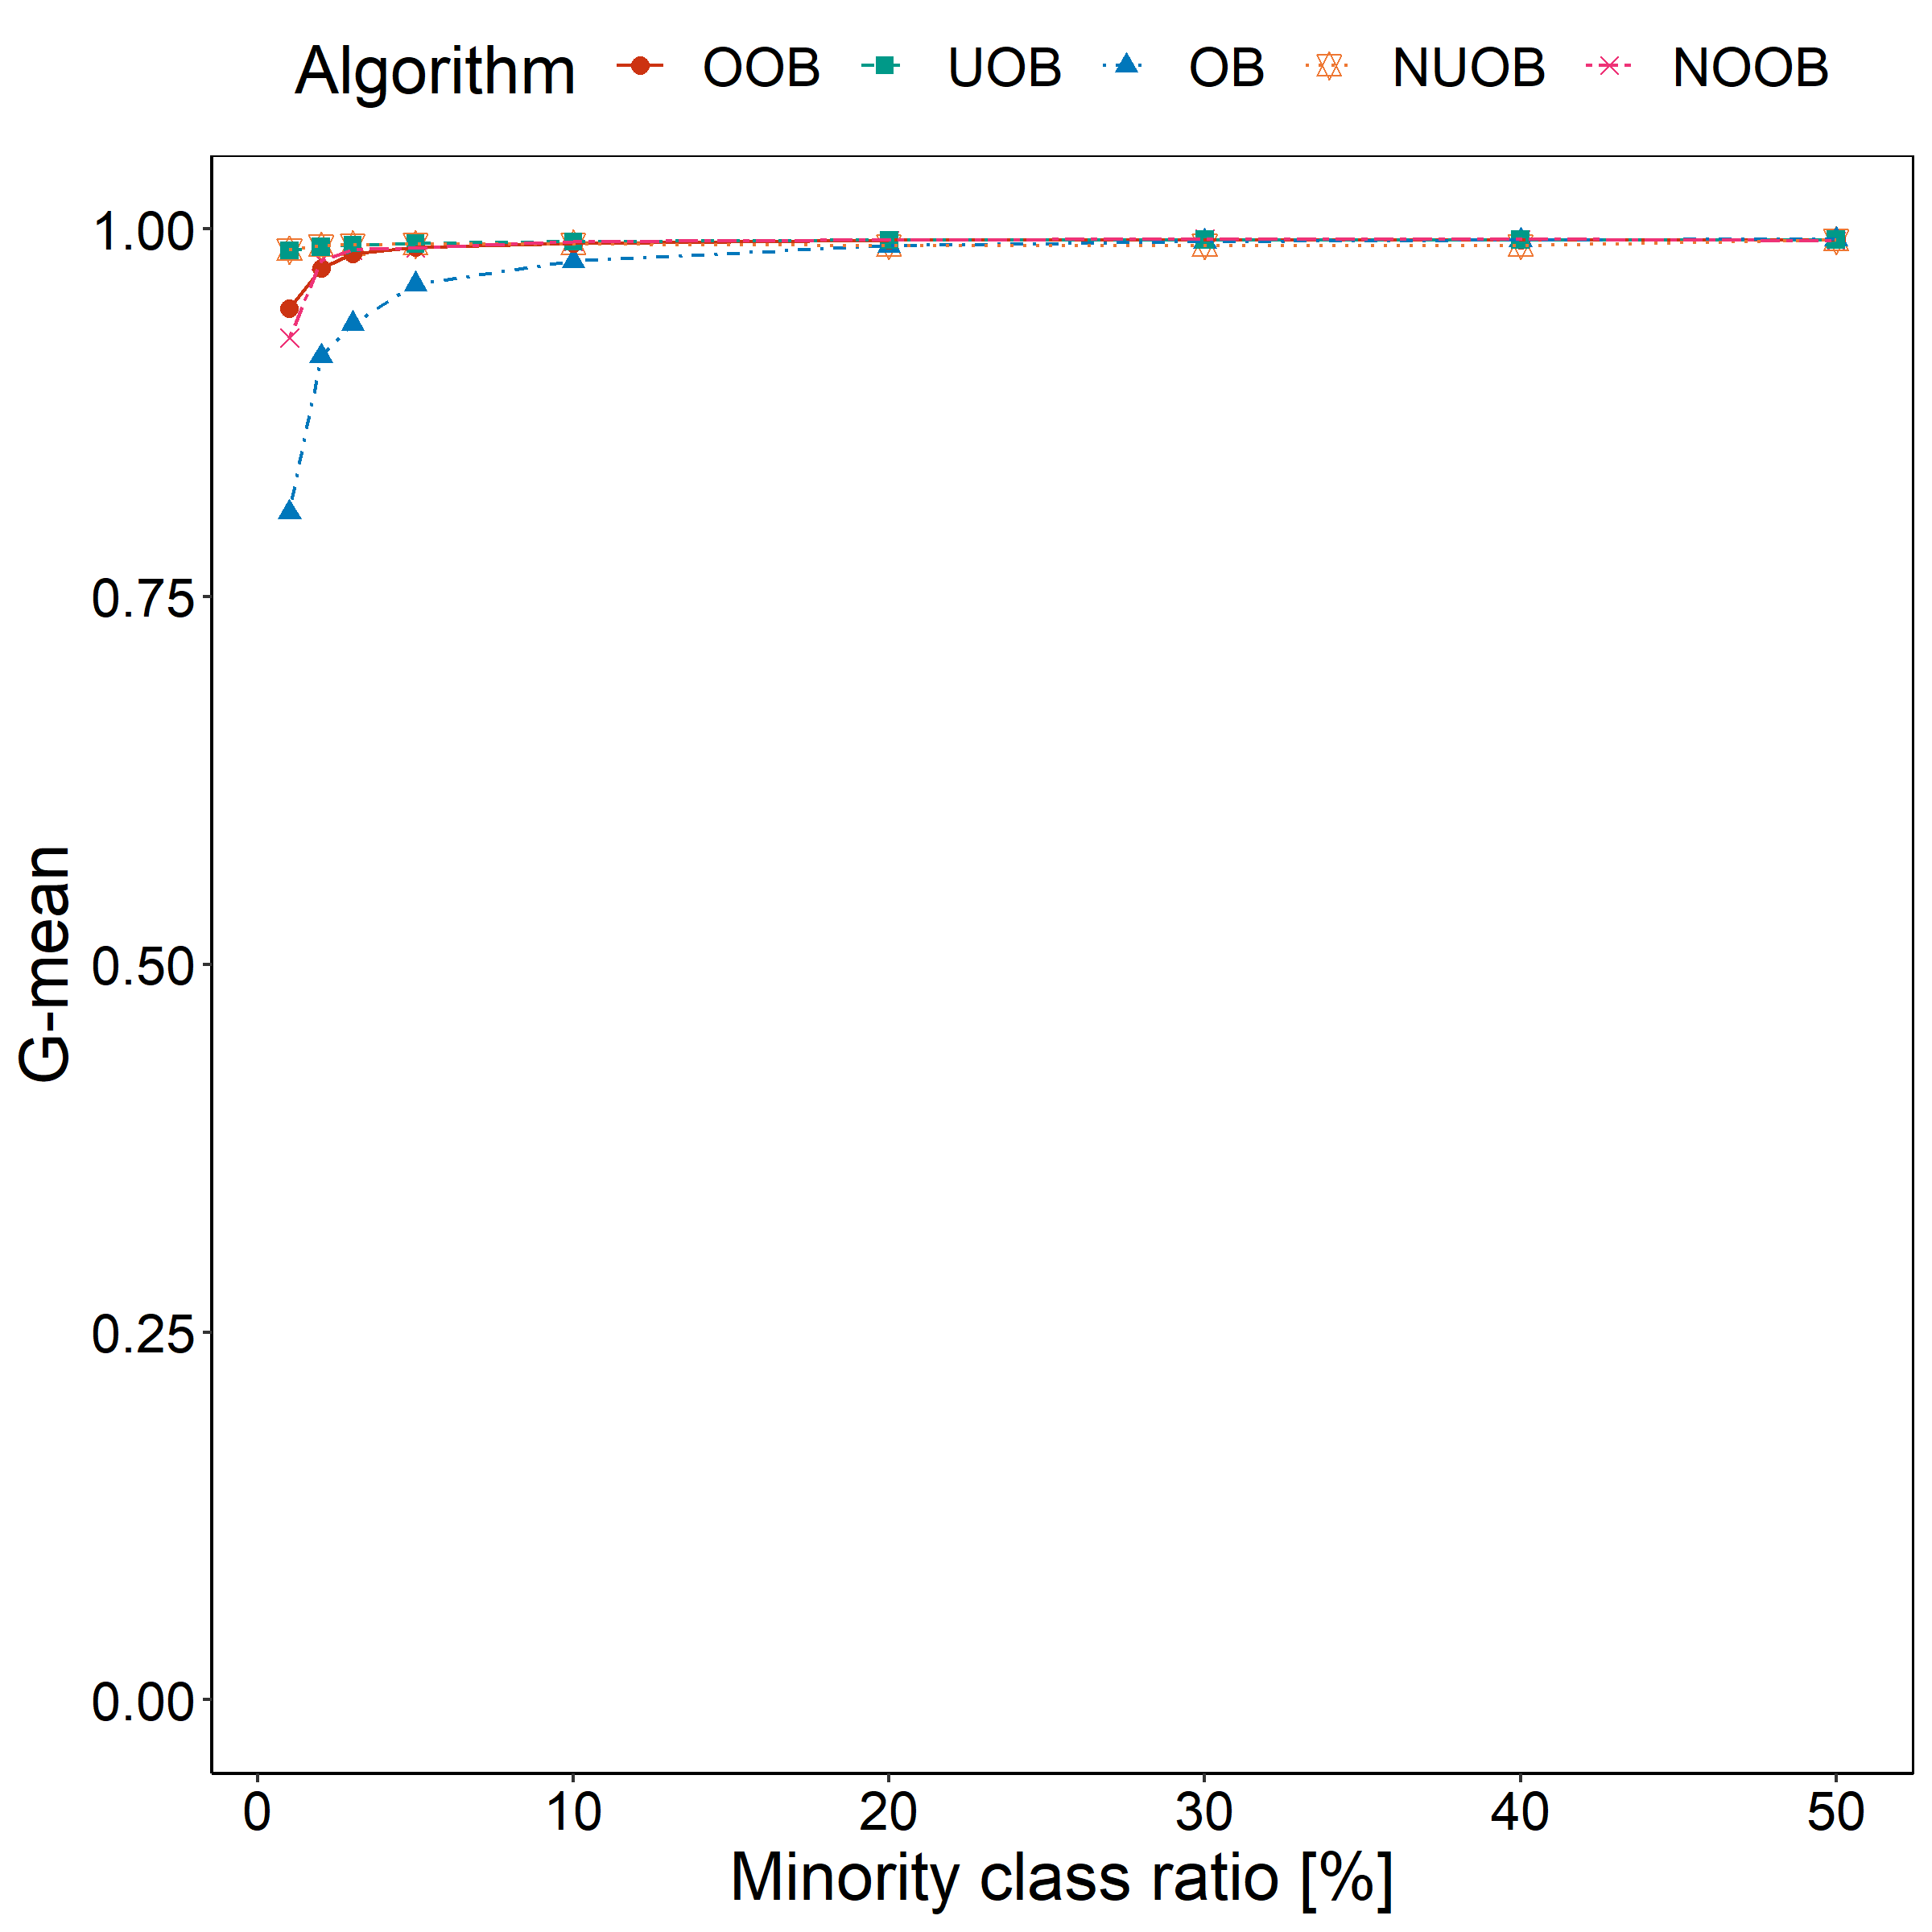
\includegraphics[width=7cm]{figures/imbalance_plot_G-mean.png}}
    \qquad
    \subfloat{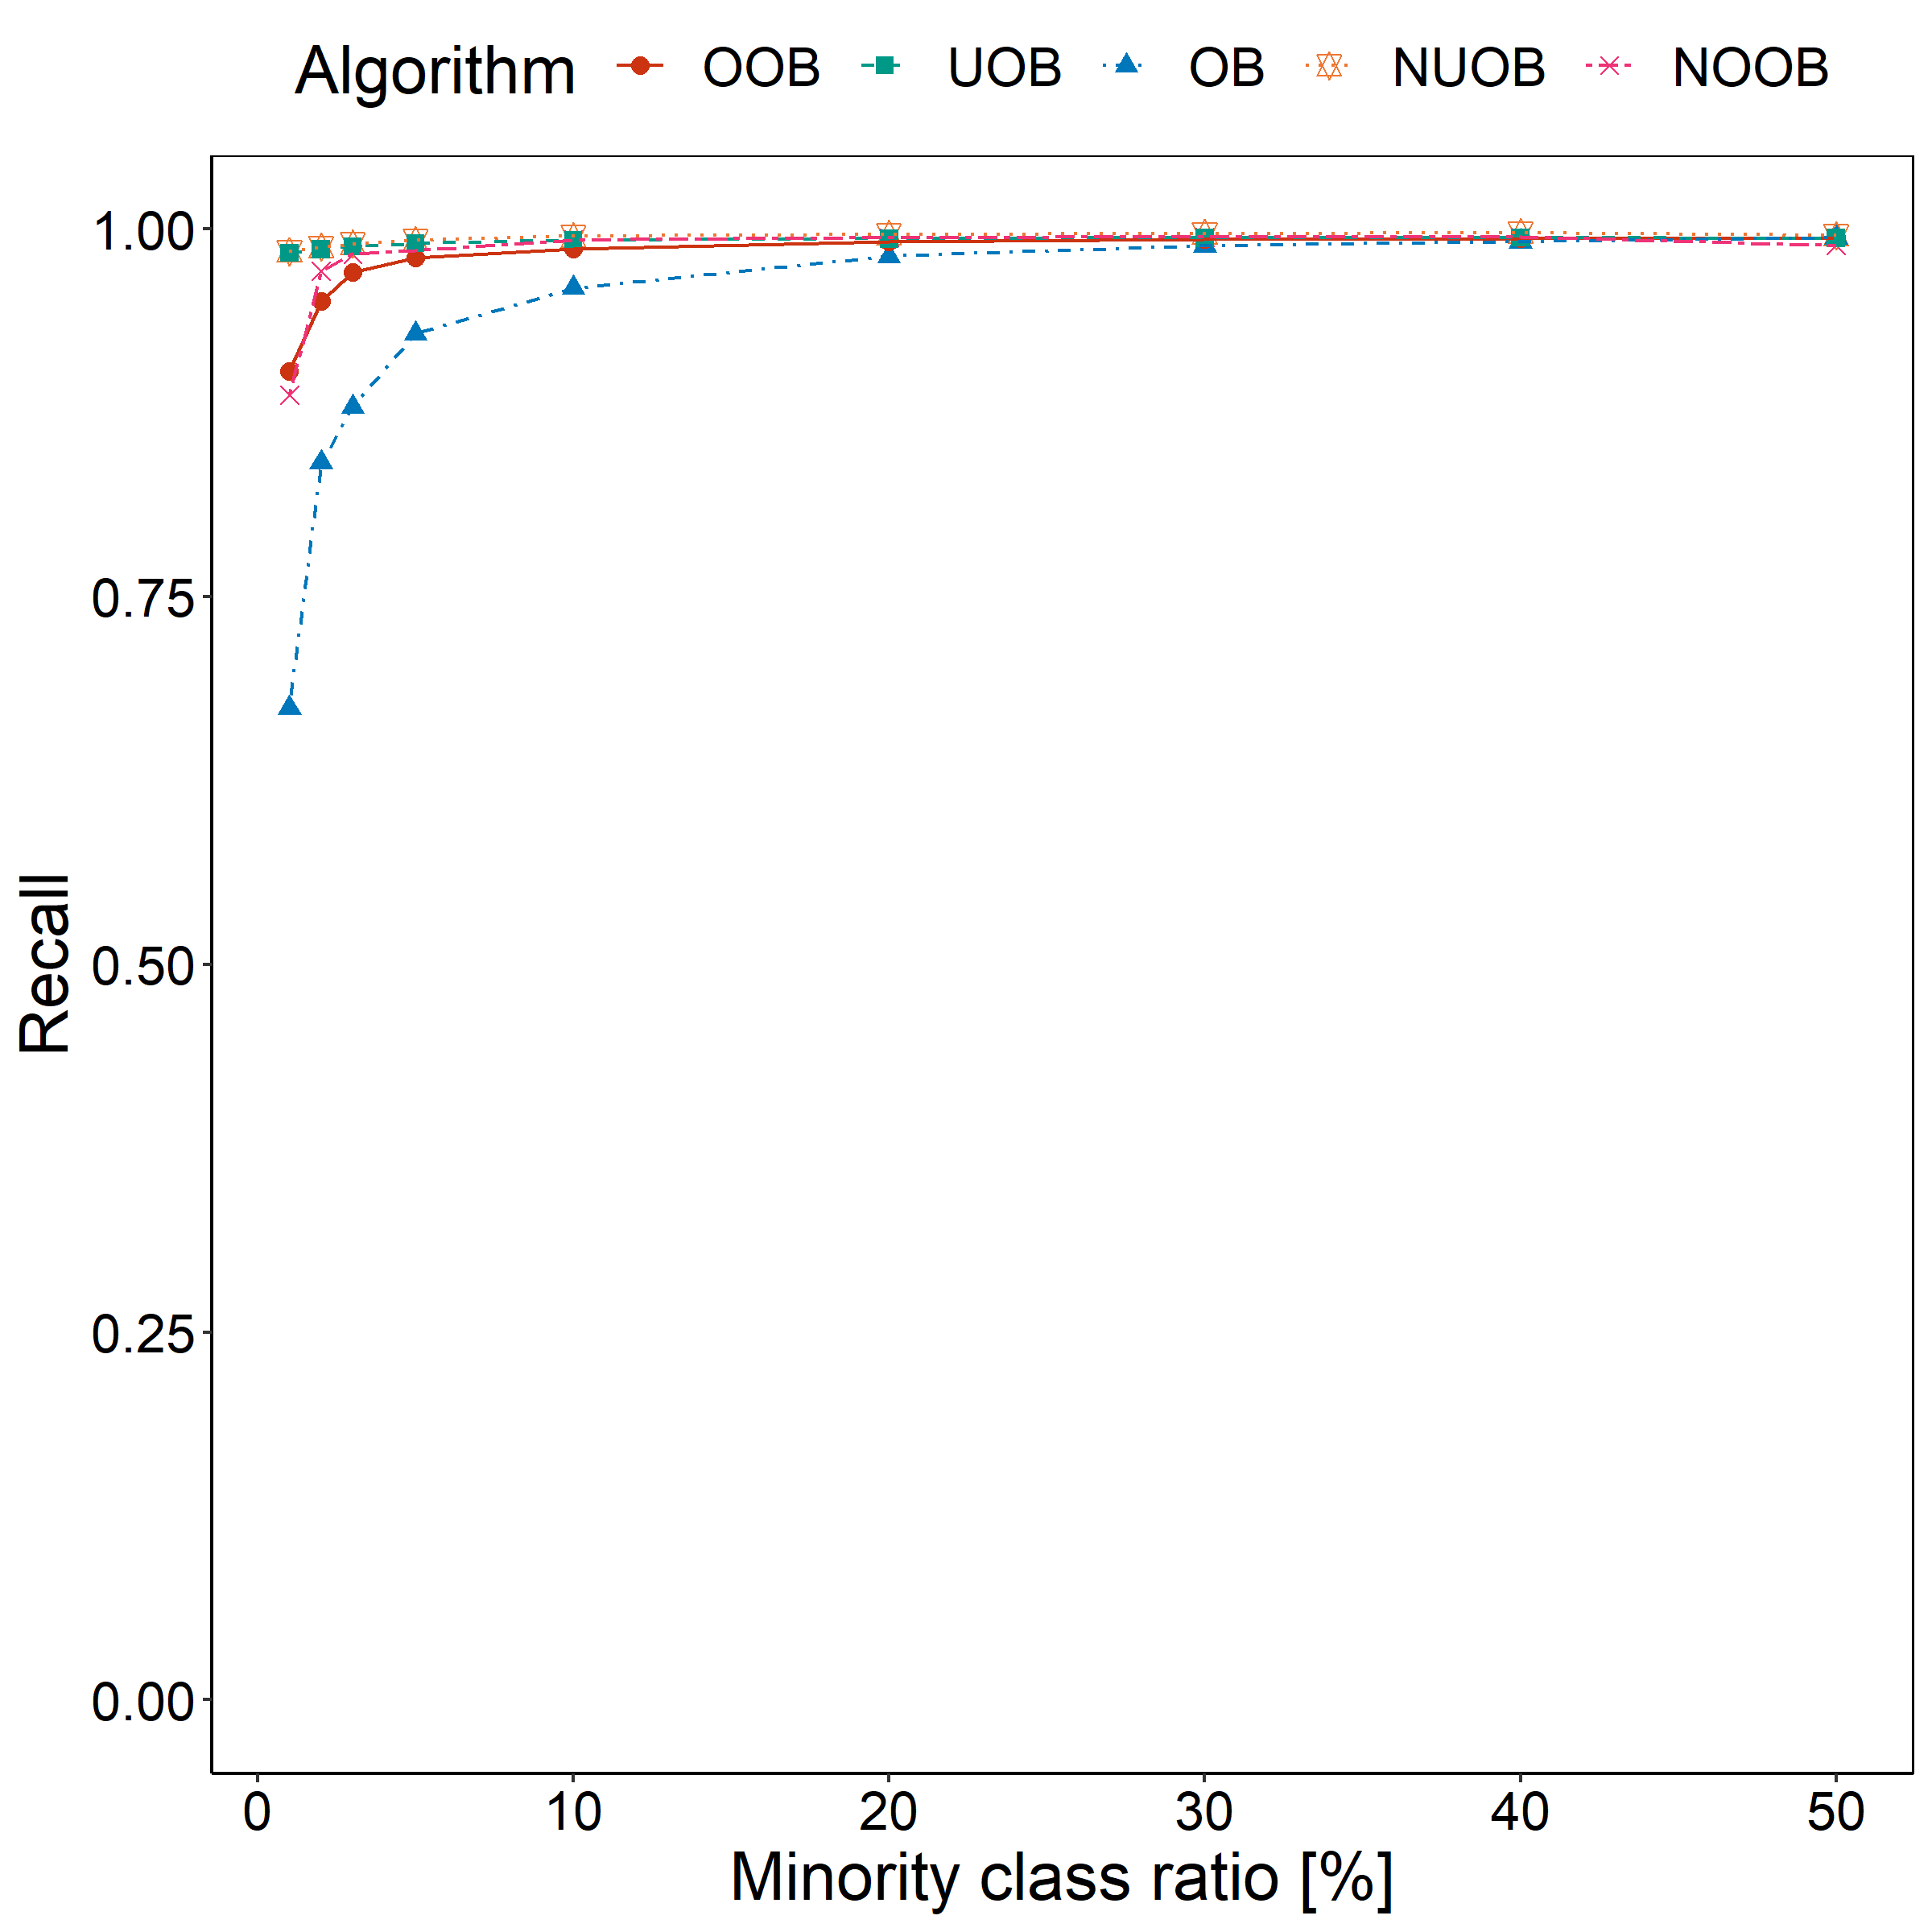
\includegraphics[width=7cm]{figures/imbalance_plot_Recall.png}}
    \caption{Porównanie jakości klasyfikacji dla różnych wartości współczynników niezbalansowania}\label{Figure:StaticImbalance}
\end{figure}

\newpage

\begin{table}[ht]
\centering\small%
\renewcommand{\arraystretch}{1.5} 
\begin{tabular}{c c c c c c}
\toprule
Imbalance Ratio & OB & UOB & OOB & NUOB & NOOB \\
\midrule
1\% & 0.807 & 0.985 & 0.945 & 0.985 & 0.925 \\
2\% & 0.913 & 0.987 & 0.972 & 0.988 & 0.978 \\
3\% & 0.935 & 0.988 & 0.982 & 0.989 & 0.985 \\
5\% & 0.962 & 0.990 & 0.987 & 0.989 & 0.987 \\
10\% & 0.977 & 0.991 & 0.990 & 0.989 & 0.991 \\
20\% & 0.988 & 0.992 & 0.992 & 0.988 & 0.992 \\
\bottomrule
\end{tabular}
\caption{Porównanie jakości klasyfikacji miary \textit{G-mean} w zależności od wartości współczynnika niezbalansowania}\label{Tab:ImbalanceRatio}
\end{table}

\noindent \textbf{Dryf pojęć ze zmianą współczynnika niezbalansowania}\\

\noindent Drugim z analizowanych czynników trudności będzie dryf pojęć ze zmianą współczynnika niezbalansowania (\textit{Im}). W przypadku wystąpienia dryfu związanego ze zmniejszeniem wartości współczynnika niezbalansowania można zaobserwować podobną sytuację, co przy analizie strumieni ze stałą wartością. Wszystkie klasyfikatory radzą sobie bardzo dobrze ze zmianami, jeśli przed wystąpieniem zjawiska dryfu współczynnik niezbalansowania wynosił przynajmniej 20\%. Sytuacja ta zaczyna się zmieniać, gdy przykładów do nauki było mniej przed wystąpieniem dryfu. Można zauważyć, że dla tych przypadków najgorzej radził sobie algorytm \textit{OB}. Pozostałe algorytmy także zaliczyły lekki spadek jakości klasyfikacji, jednak nadal utrzymywał się on koło wartości 0.98 dla miary \textit{G-mean} dla najlepszych algorytmów \textit{UOB} oraz \textit{NUOB}.

Sytuacja zmienia się w przypadku zaobserwowania dryfu związane ze zwiększeniem się wartości współczynnika niezbalansowania. Największy spadek jakości klasyfikacji dla algorytmów można zaobserwować dla przypadku, gdzie przed wystąpieniem dryfu pojęć liczba przykładów z klasy mniejszościowej stanowi zaledwie 1\% wszystkich przykładów. Najgorzej spisującym się algorytmem w tym przypadku był \textit{OB}, lekki spadek widoczny jest także dla algorytmów \textit{NOOB} oraz \textit{OOB}.

Podsumowując, zaprezentowane algorytmy w większości przypadków radzą sobie bardzo dobrze ze zjawiskiem zmiany współczynnika niezbalansowania. Dla najbardziej wymagających scenariuszy, gdzie przykładów z klasy mniejszościowej przed dryfem jest bardzo mało, można zaobserwować lekkie spadki jakości klasyfikacji dla średniej wartości miary \textit{G-mean}, jednak spadki te nie są bardzo duże. Zbiorowe wyniki klasyfikacji zostały przedstawione na rysunku \ref{Figure:DriftImbalance}. Jak można zauważyć na ilustracji \ref{Figure:StaticIm1_Im60} przedstawiającej scenariusz \textit{StaticIm1+Im60}, głównym problemem w procesie uczenia jest mała ilość przykładów z klasy mniejszościowej. Po wystąpieniu dryfu można zaobserwować, że jakość klasyfikacji wzrasta i utrzymuje się na poziomie wartości 0.99 dla obu badanych miar. W przypadku scenariuszy charakteryzujących się spadkiem współczynnika niezbalansowania (zaprezentowanych na ilustracji \ref{Figure:StaticIm10_Im1}), tak jak się można  spodziewać, widoczne jest obniżenie jakości klasyfikacji dla algorytmów po wystąpieniu dryfu. Mimo chwilowego spadku wszystkie algorytmy reagują odpowiednio na zmiany i ostatecznie wracają do poziomu, który występował przed dryfem.

\begin{figure}[h]
    \centering
    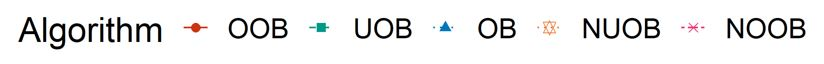
\includegraphics[width=7cm]{figures/algorithms_legend.JPG}
\end{figure}

\vspace{-1.2cm}

\begin{figure}[h]
    \centering
    \subfloat{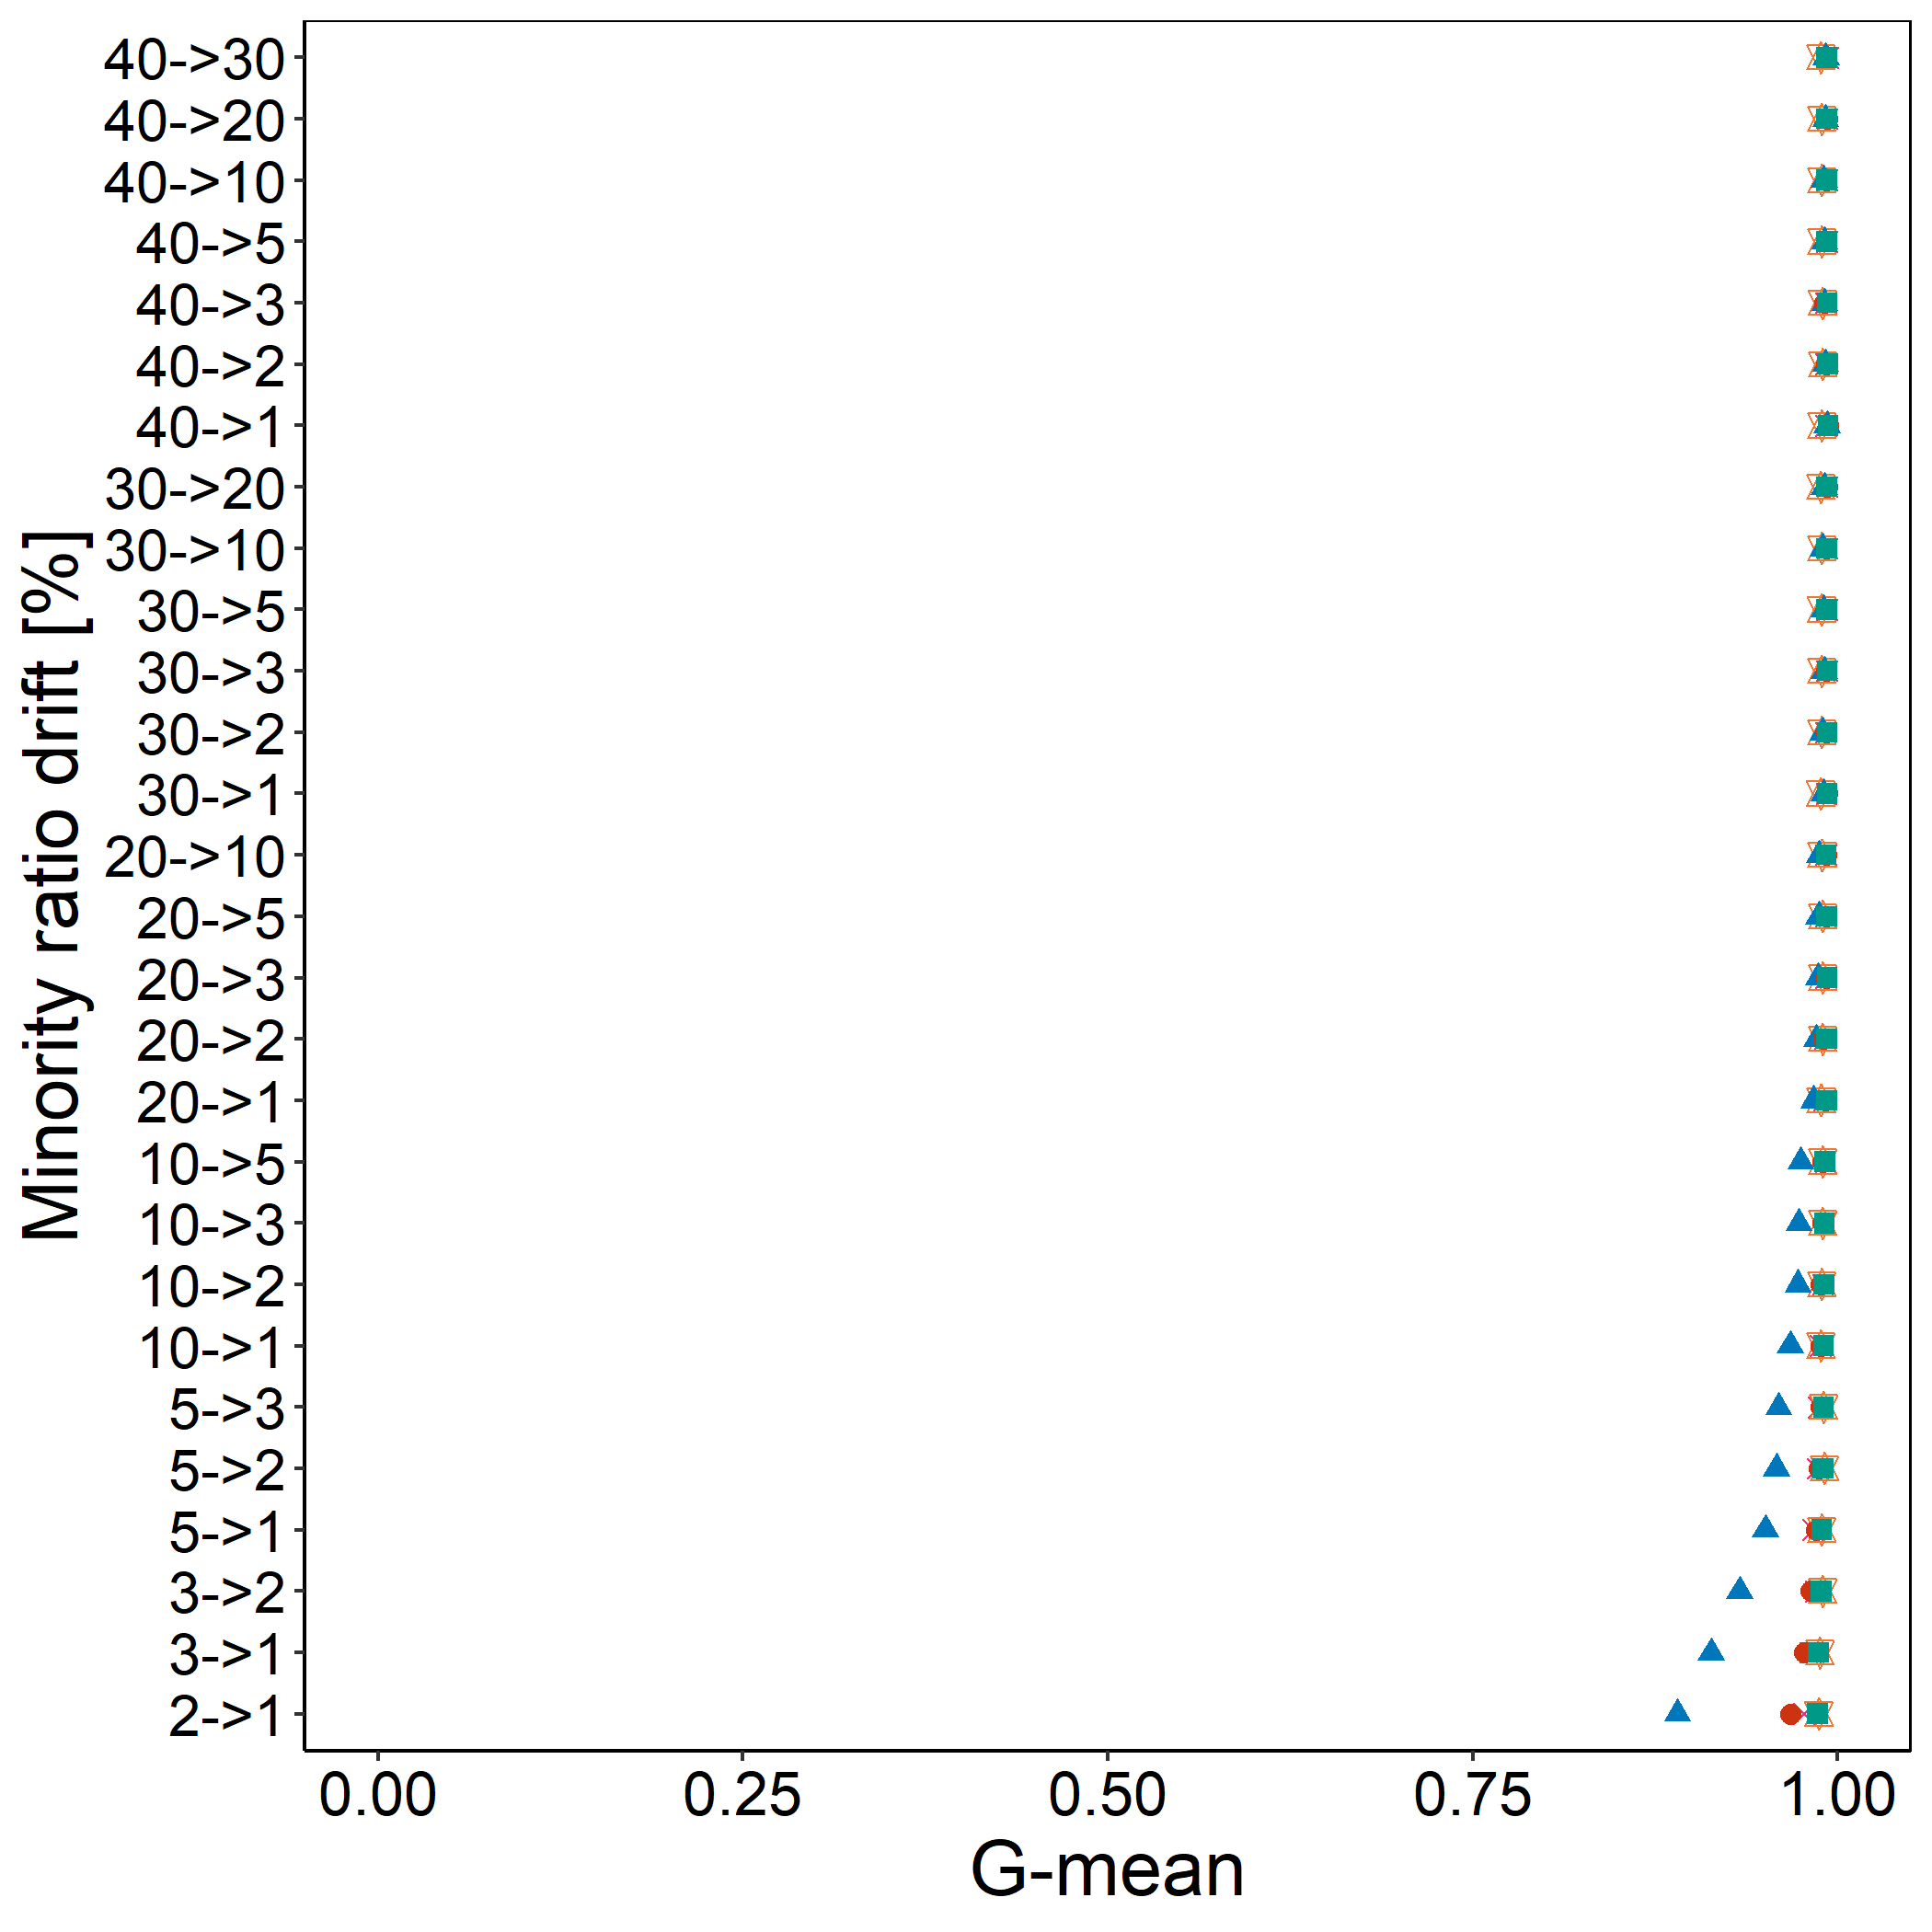
\includegraphics[width=7cm]{figures/dynamic_decreasing_plot_G-mean.png}}
    \qquad
    \subfloat{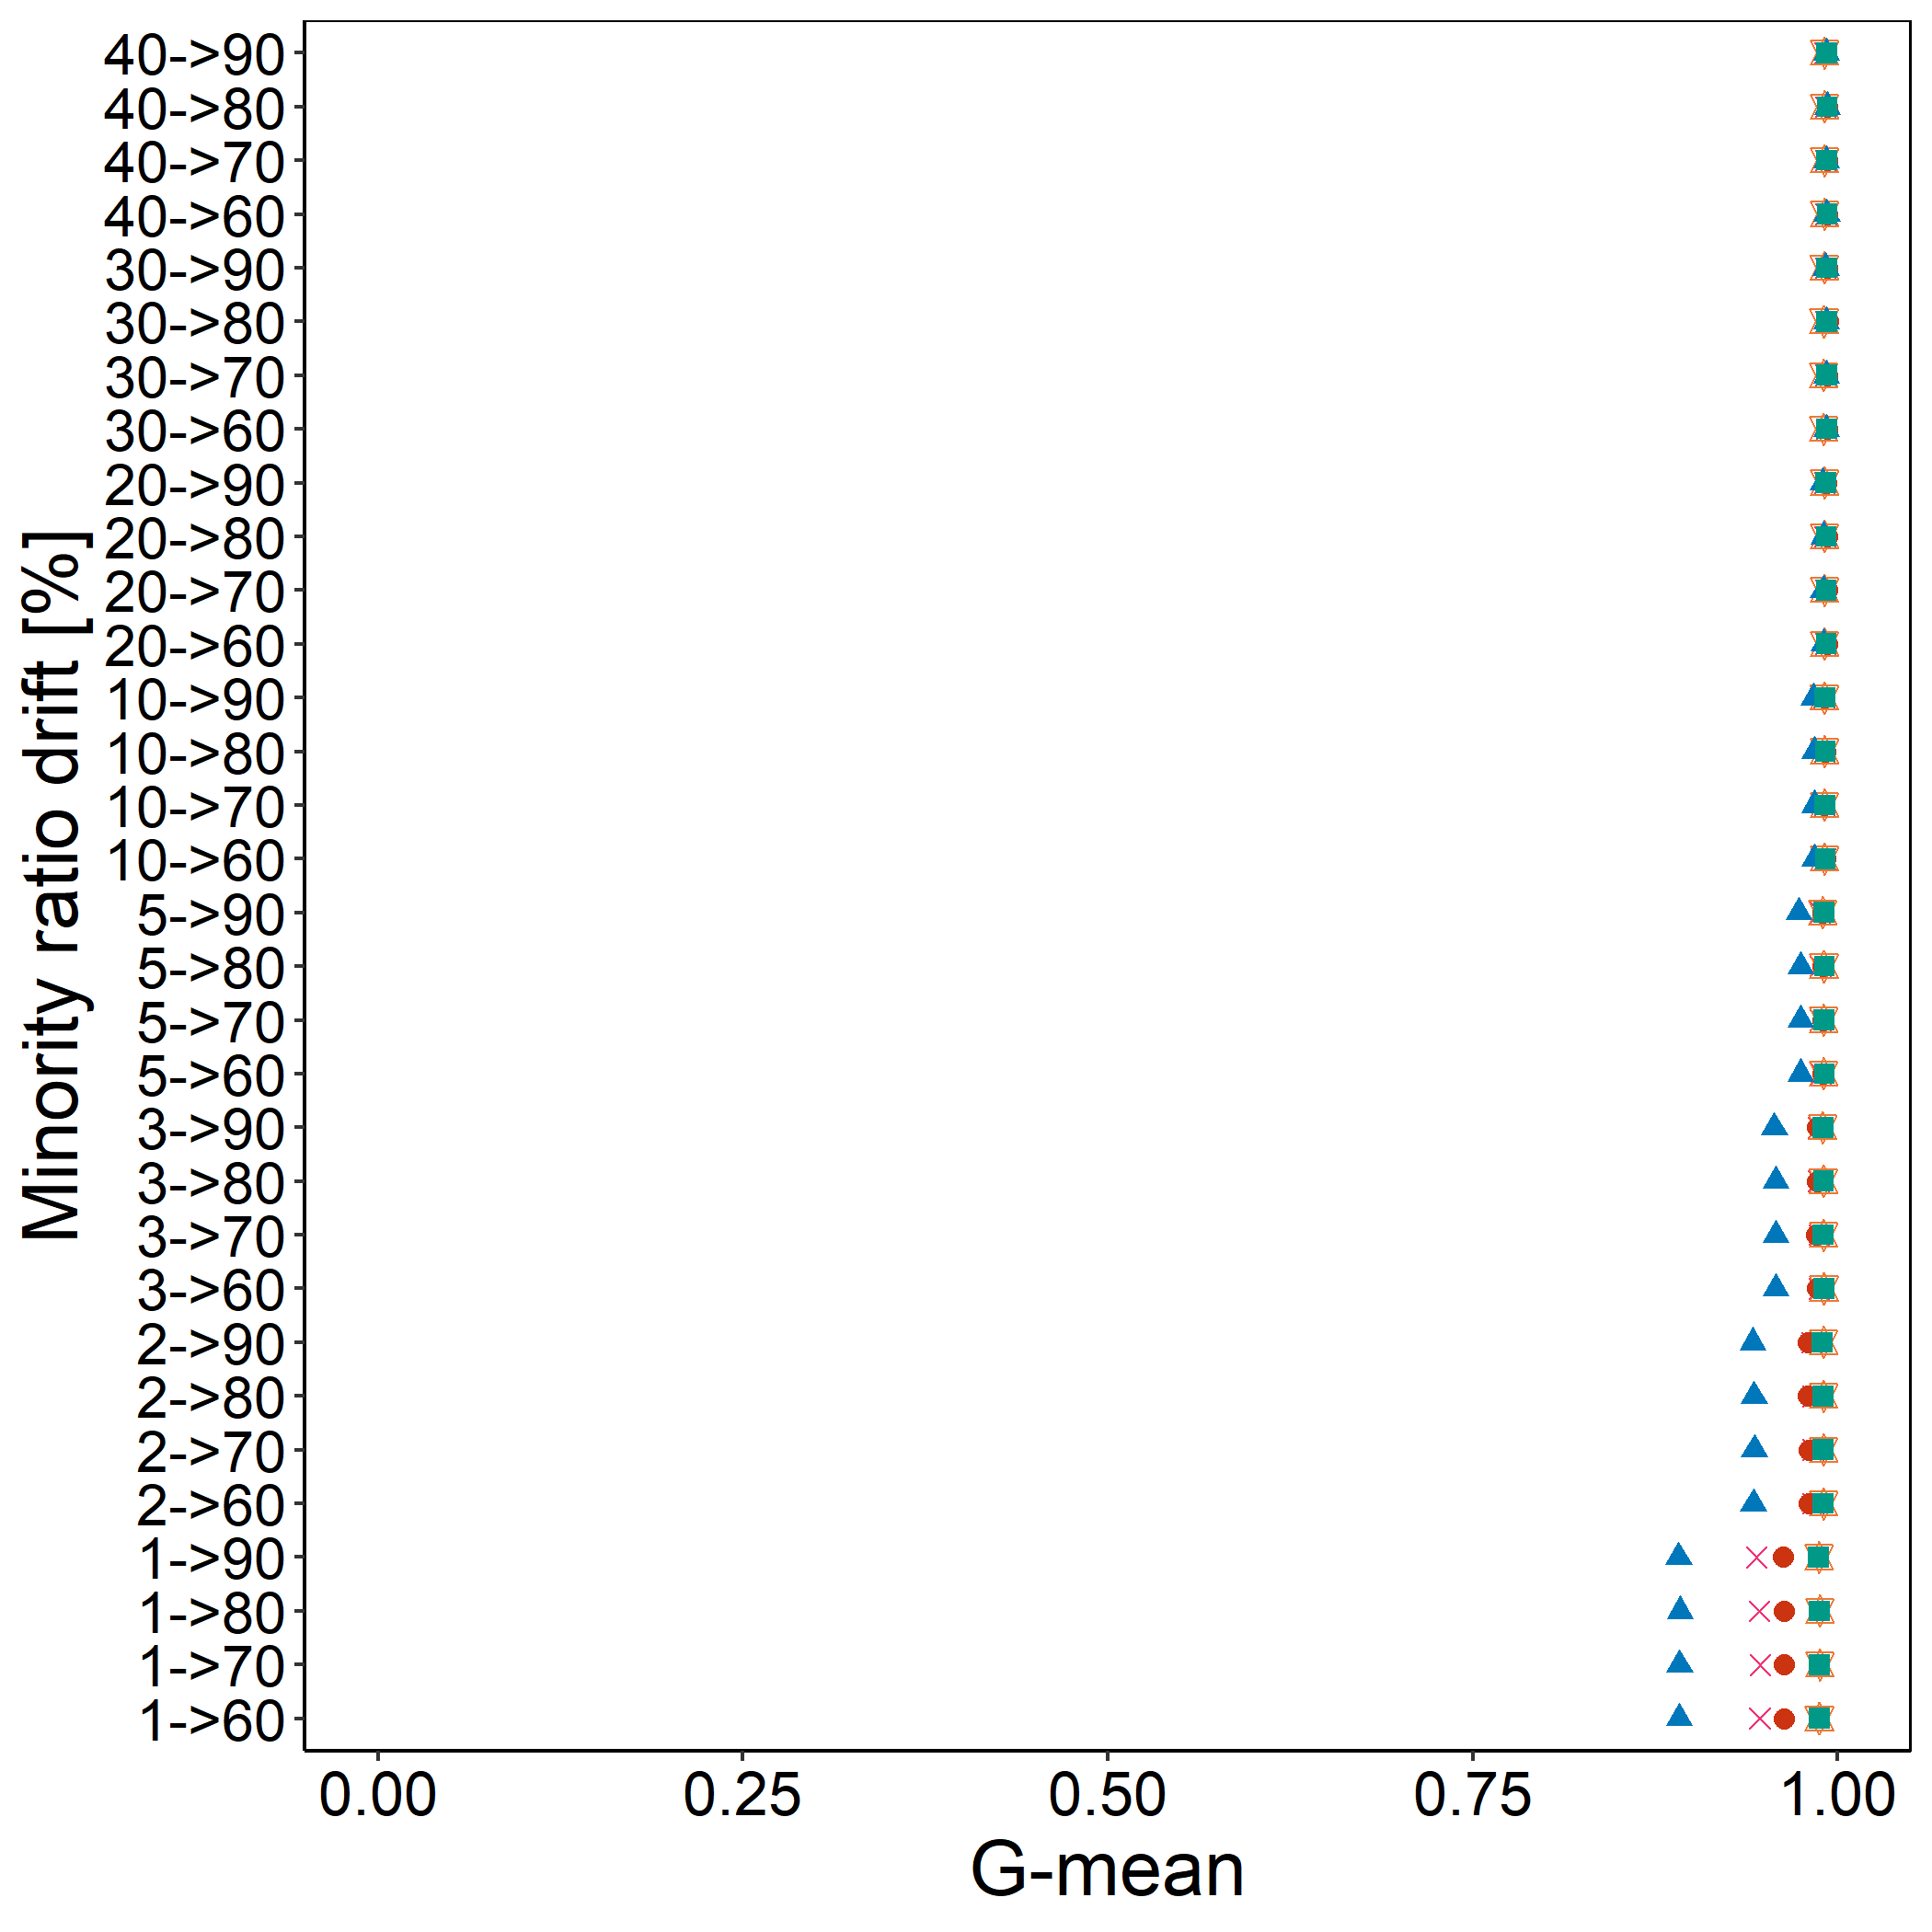
\includegraphics[width=7cm]{figures/dynamic_increasing_plot_G-mean.png}}
    \caption{Porównanie jakości klasyfikacji przy zmianie współczynnika niezbalansowania podczas zjawiska dryfu}\label{Figure:DriftImbalance}
\end{figure}

\begin{figure}[h]
    \centering
    \subfloat{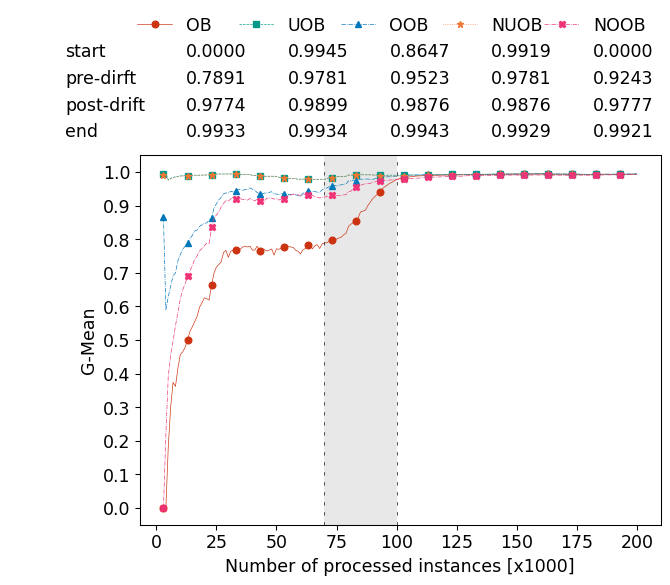
\includegraphics[width=7cm]{figures/staticim1_im60_gmean.png}}
    \qquad
    \subfloat{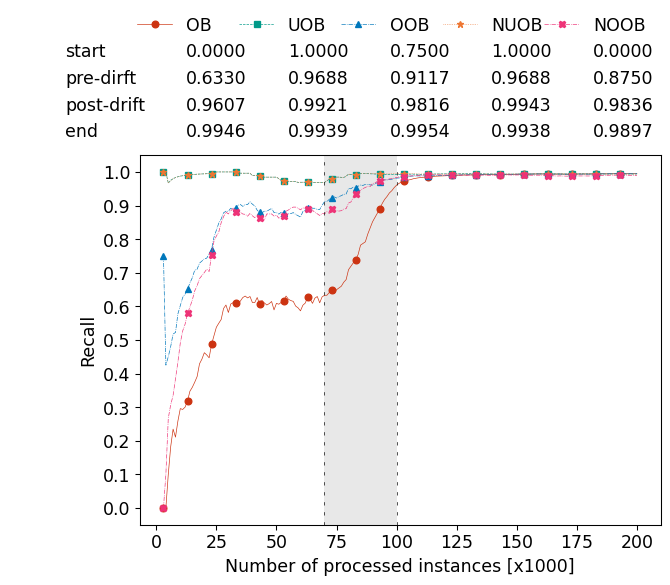
\includegraphics[width=7cm]{figures/staticim1_im60_recall.png}}
    \caption{Wykresy liniowe miar \textit{G-mean} oraz \textit{Recall} dla strumienia \textit{StaticIm1+Im60}}\label{Figure:StaticIm1_Im60}
\end{figure}

\newpage

\begin{figure}[h]
    \centering
    \subfloat{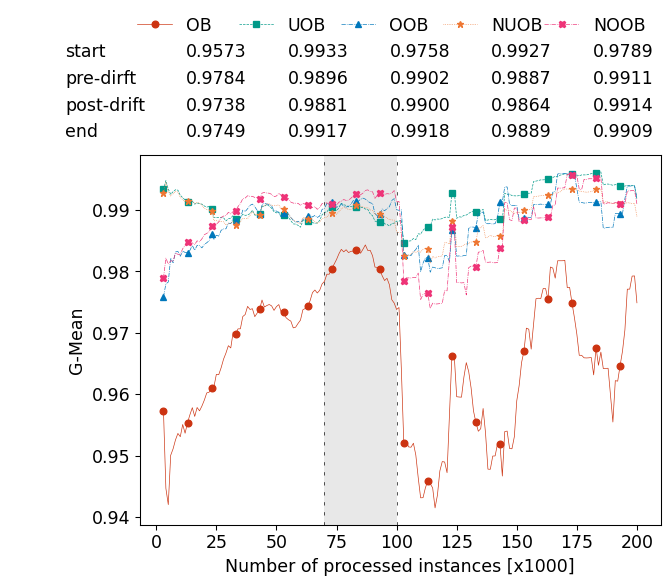
\includegraphics[width=7cm]{figures/staticim10_im1_gmean.png}}
    \qquad
    \subfloat{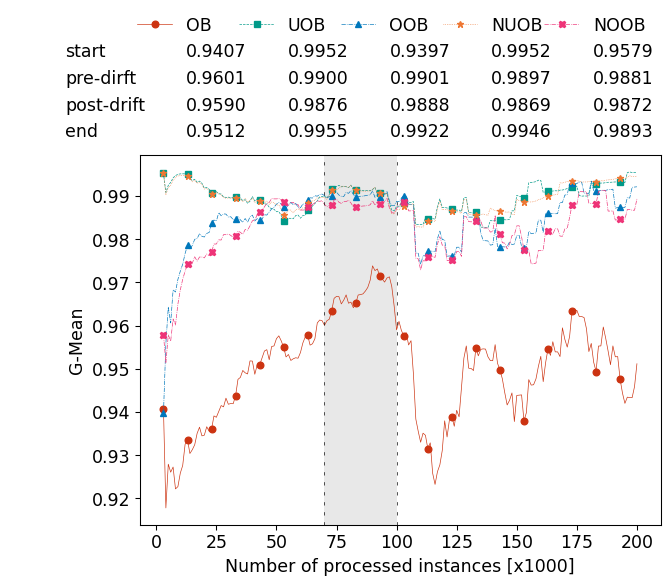
\includegraphics[width=7cm]{figures/staticim5_im1_gmean.png}}
    \caption{Wykresy liniowe miary \textit{G-mean} dla strumieni \textit{StaticIm10+Im1} (po lewej) oraz \textit{StaticIm5+Im1} (po prawej)}\label{Figure:StaticIm10_Im1}
\end{figure}

\vspace{0.7cm}

\noindent \textbf{Zmiana rozkładu klasy mniejszościowej}\\

\noindent Trzecim z analizowanych czynników trudności będzie zmiana rozkładu klasy mniejszościowej. Czynnik ten powiązany jest ze zmianą pozycji skupisk przykładów klasy mniejszościowej. Obejmuje następujące scenariusze:

\begin{itemize}
    \item Podział skupiska przykładów klasy mniejszościowej na mniejsze grupy przykładów (\textit{Split})
    \item Przesuwanie się skupisk w przestrzeni atrybutów (\textit{Move})
    \item Połączenie grup przykładów klasy mniejszościowej w jedno większe skupisko (\textit{Merge})
\end{itemize}

\begin{figure}[h]
    \centering
    \subfloat{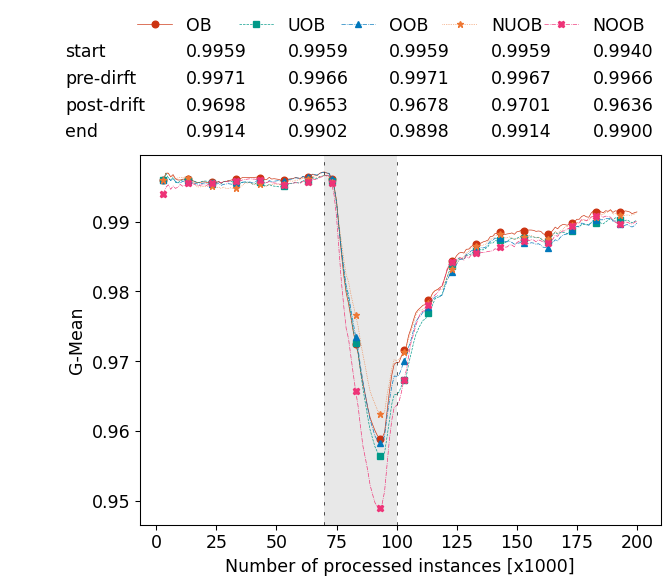
\includegraphics[width=7cm]{figures/split5_gmean.png}}
    \qquad
    \subfloat{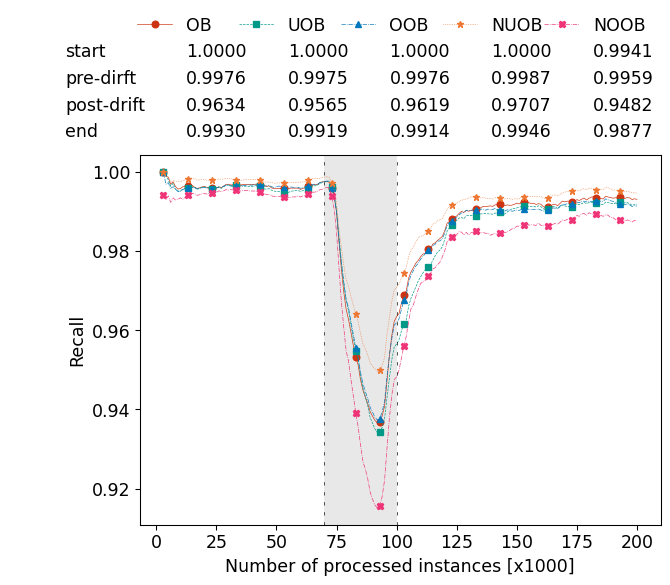
\includegraphics[width=7cm]{figures/split5_recall.png}}
    \caption{Wykresy liniowe miar \textit{G-mean} oraz \textit{Recall} dla strumienia \textit{Split5}}\label{Figure:Split5}
\end{figure}

\noindent W przypadku scenariusza związanego z podziałem skupiska można zauważyć spadek w jakości klasyfikacji w trakcie występowania dryfu pojęć. Jak można zauważyć większość klasyfikatorów zachowała się bardzo podobnie. Po zaobserwowanym spadku widoczny jest wzrost, który świadczy o tym, że algorytmy przystosowały się odpowiednio do zmian, które zaszły w badanym strumieniu. Identyczny efekt można zaobserwować dla scenariusza, gdy grupy przykładów przemieszczają się w przestrzeni atrybutów. W trakcie przemieszczania widoczny jest spadek wartości badanych miar, natomiast po przemieszczeniu klasyfikatory odpowiednio przystosowują się do zmian, co skutkuje wzrostem jakości klasyfikacji. Podobną sytuację można zaobserwować w przypadku połączenia grup przykładów w większe skupisko, co zostało przedstawione na rysunku \ref{Figure:Join5}.

\begin{figure}[h]
    \centering
    \subfloat{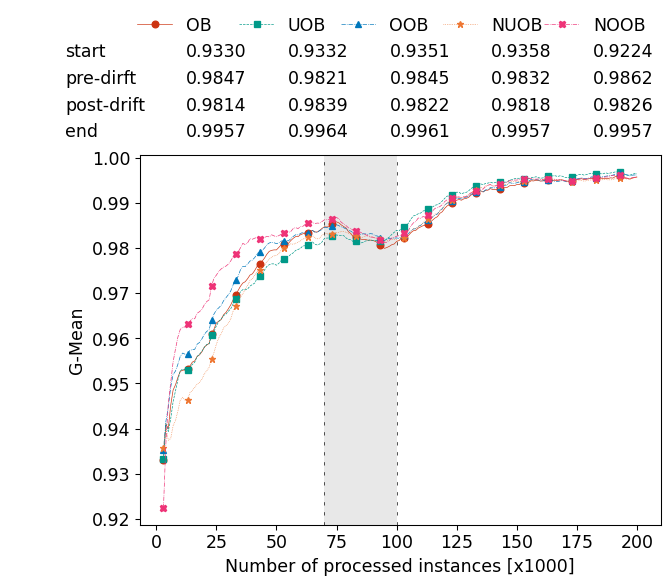
\includegraphics[width=7cm]{figures/join5_gmean.png}}
    \qquad
    \subfloat{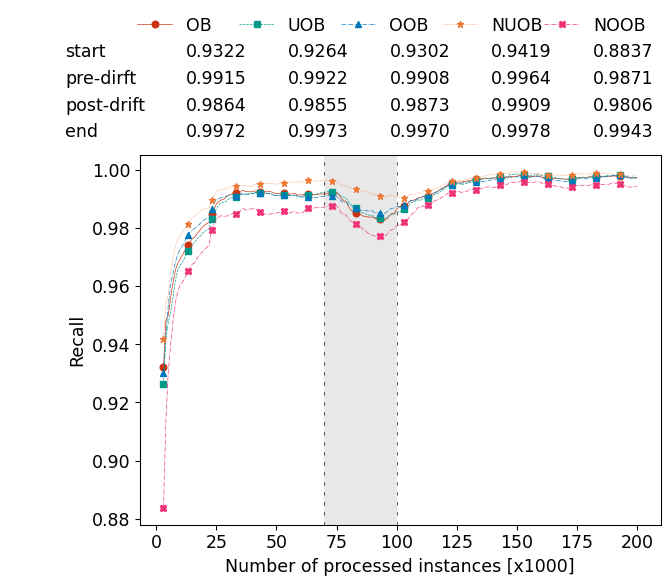
\includegraphics[width=7cm]{figures/join5_recall.png}}
    \caption{Wykresy liniowe miar \textit{G-mean} oraz \textit{Recall} dla strumienia \textit{Merge5}}\label{Figure:Join5}
\end{figure}

\begin{figure}[h]
    \centering
    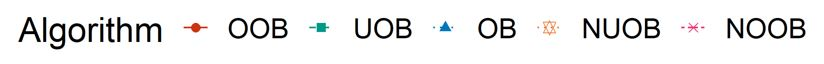
\includegraphics[width=7cm]{figures/algorithms_legend.JPG}
\end{figure}

\vspace{-1.2cm}

\begin{figure}[h]
    \centering
    \subfloat{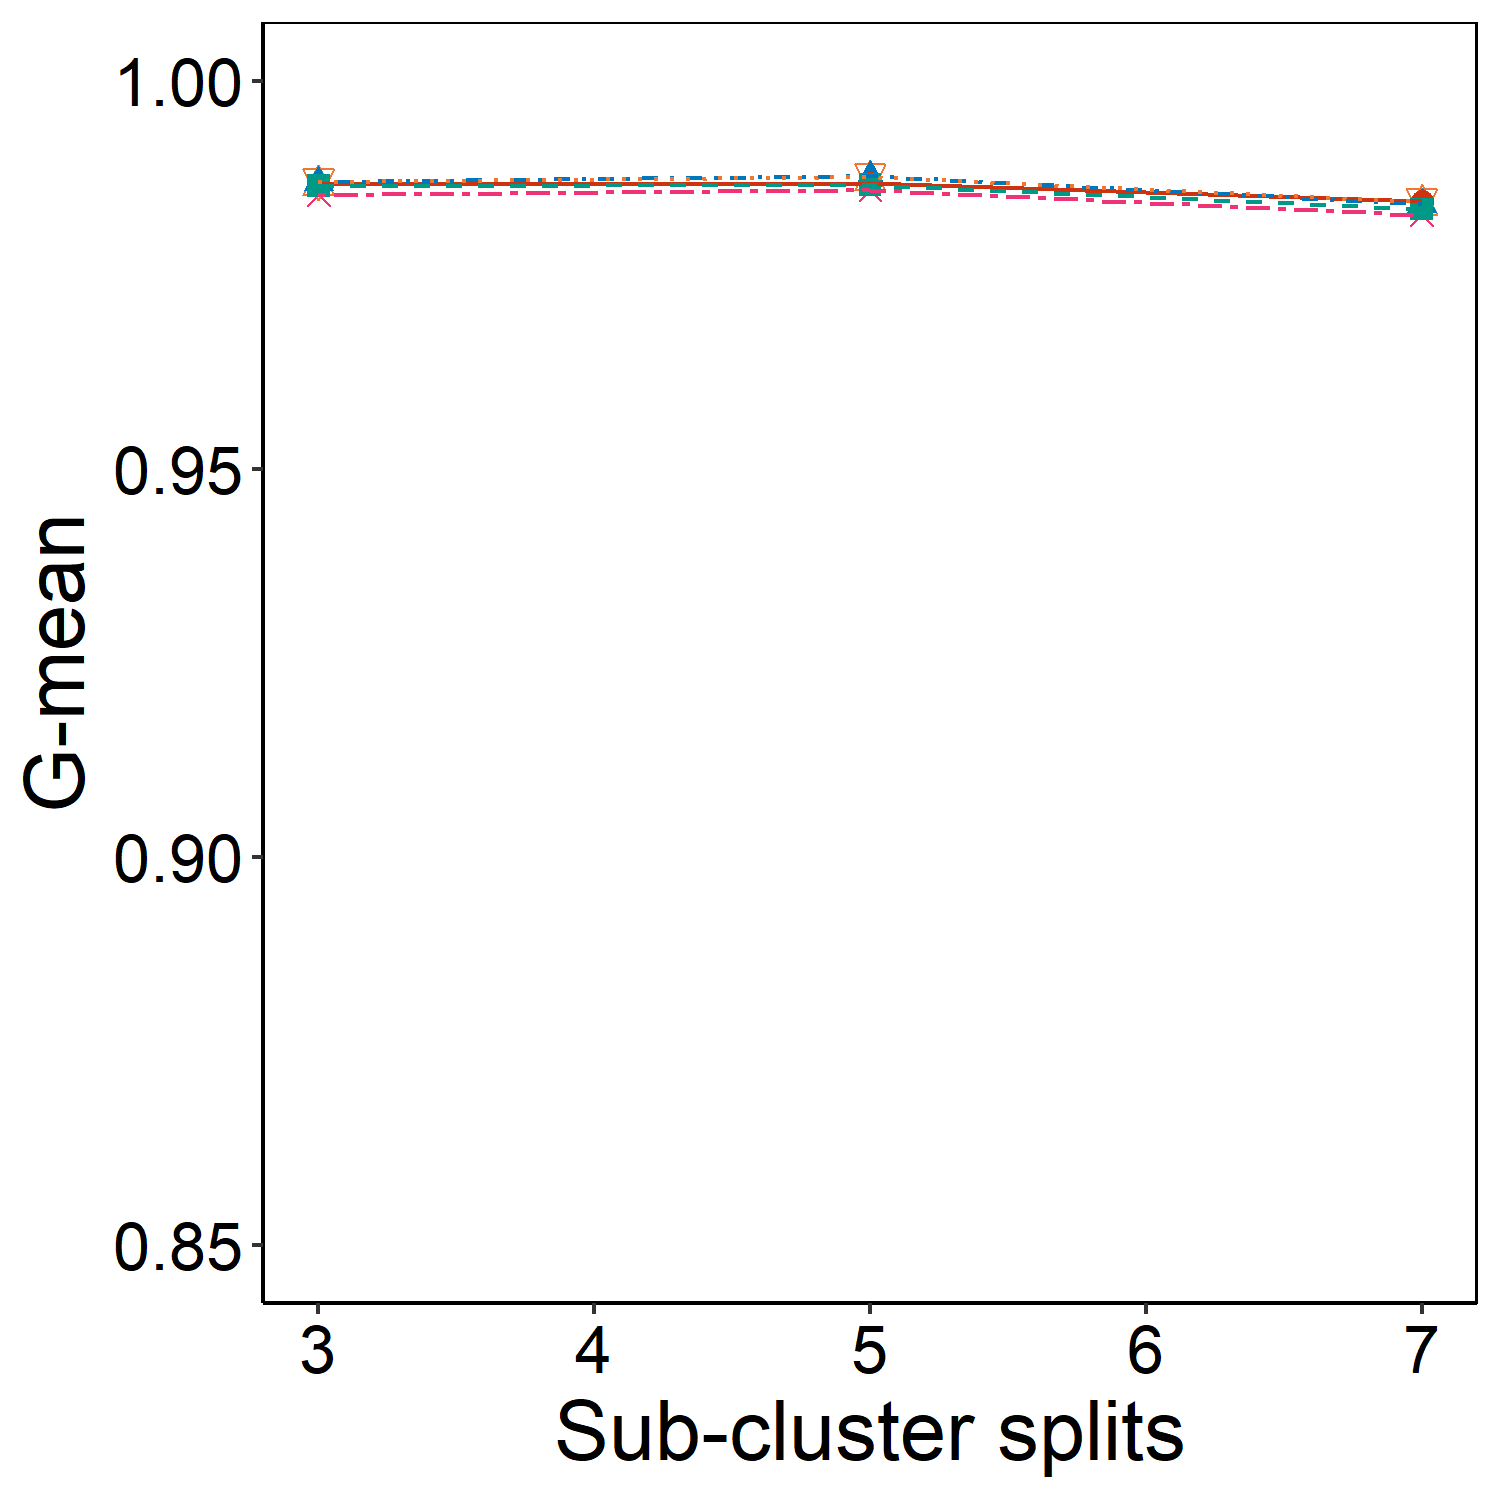
\includegraphics[width=4cm]{figures/Split_plot_G-mean.png}}
    \qquad
    \subfloat{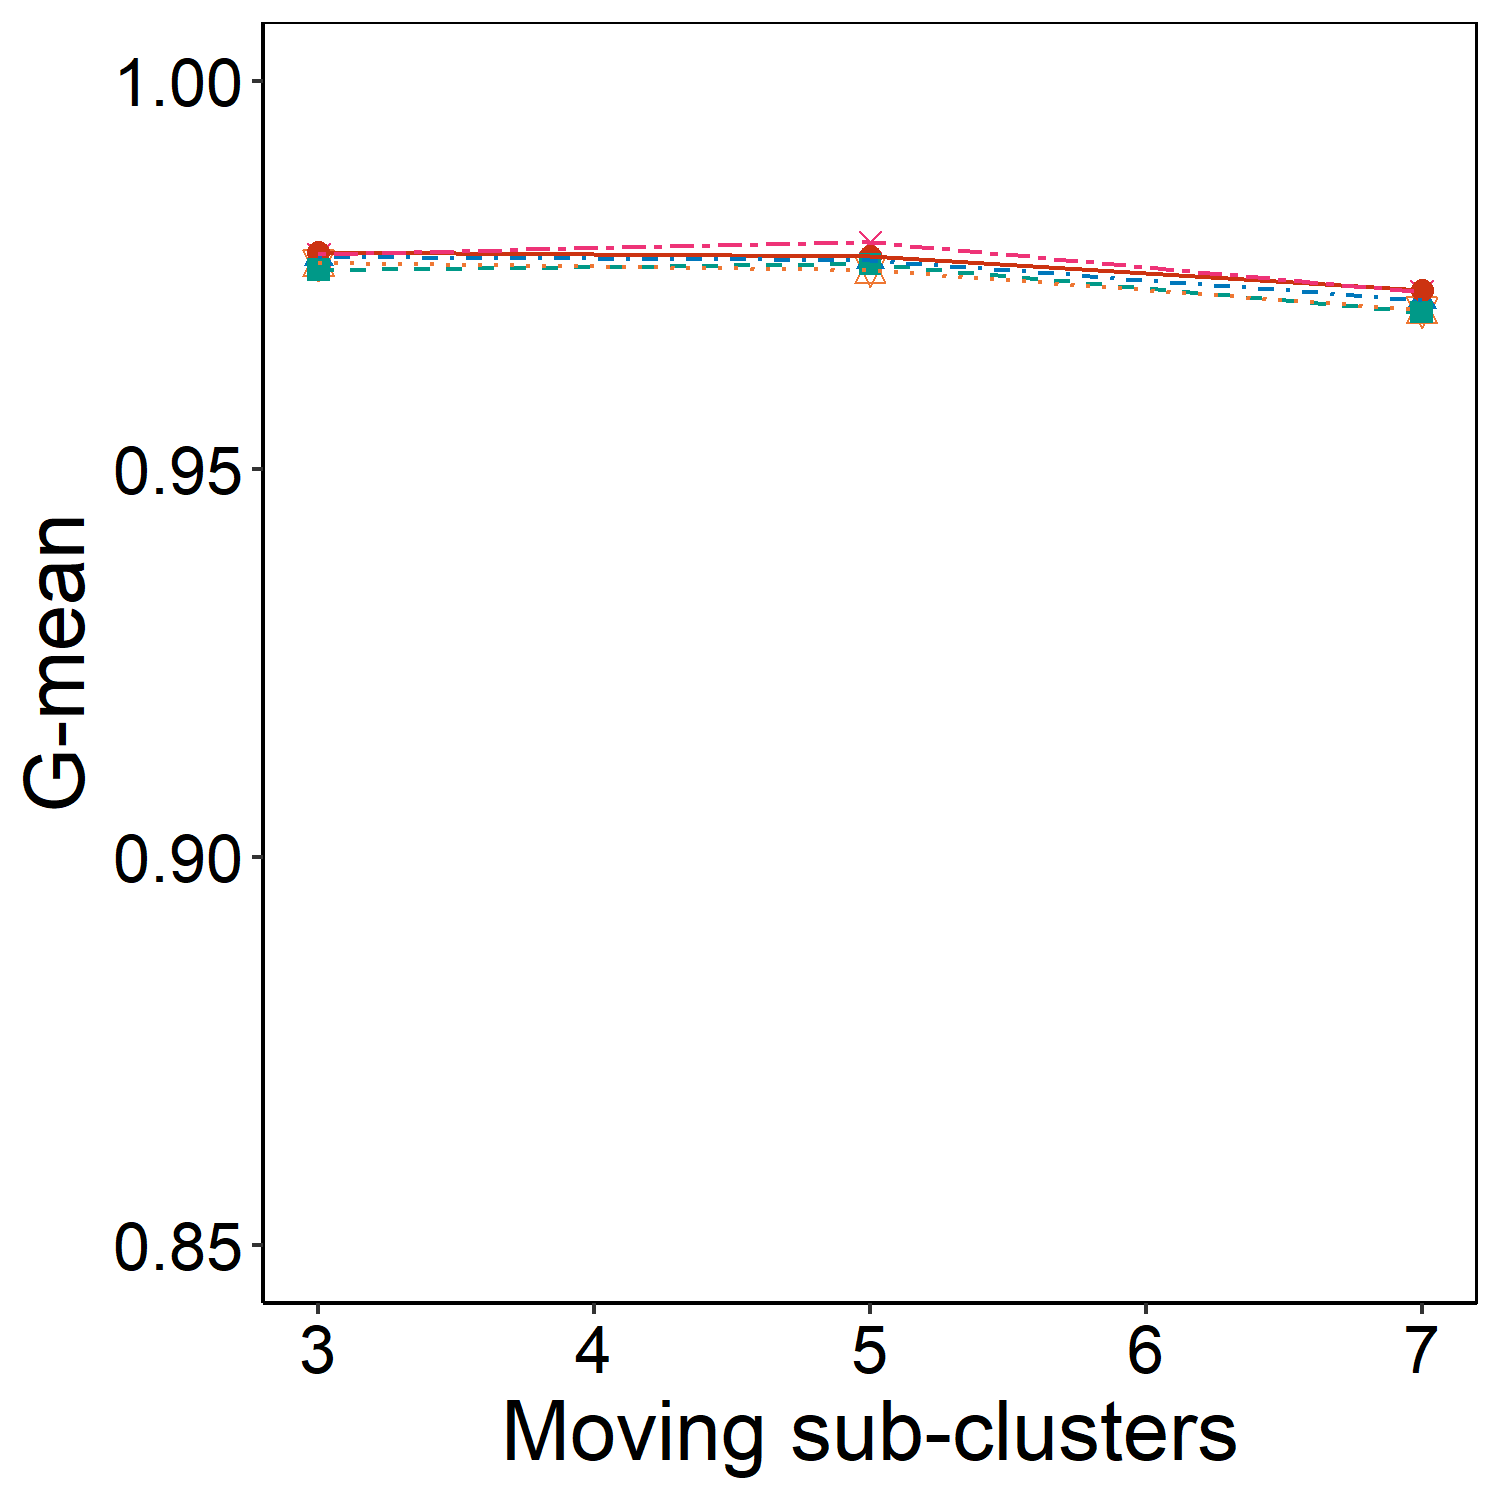
\includegraphics[width=4cm]{figures/Move_plot_G-mean.png}}
    \qquad
    \subfloat{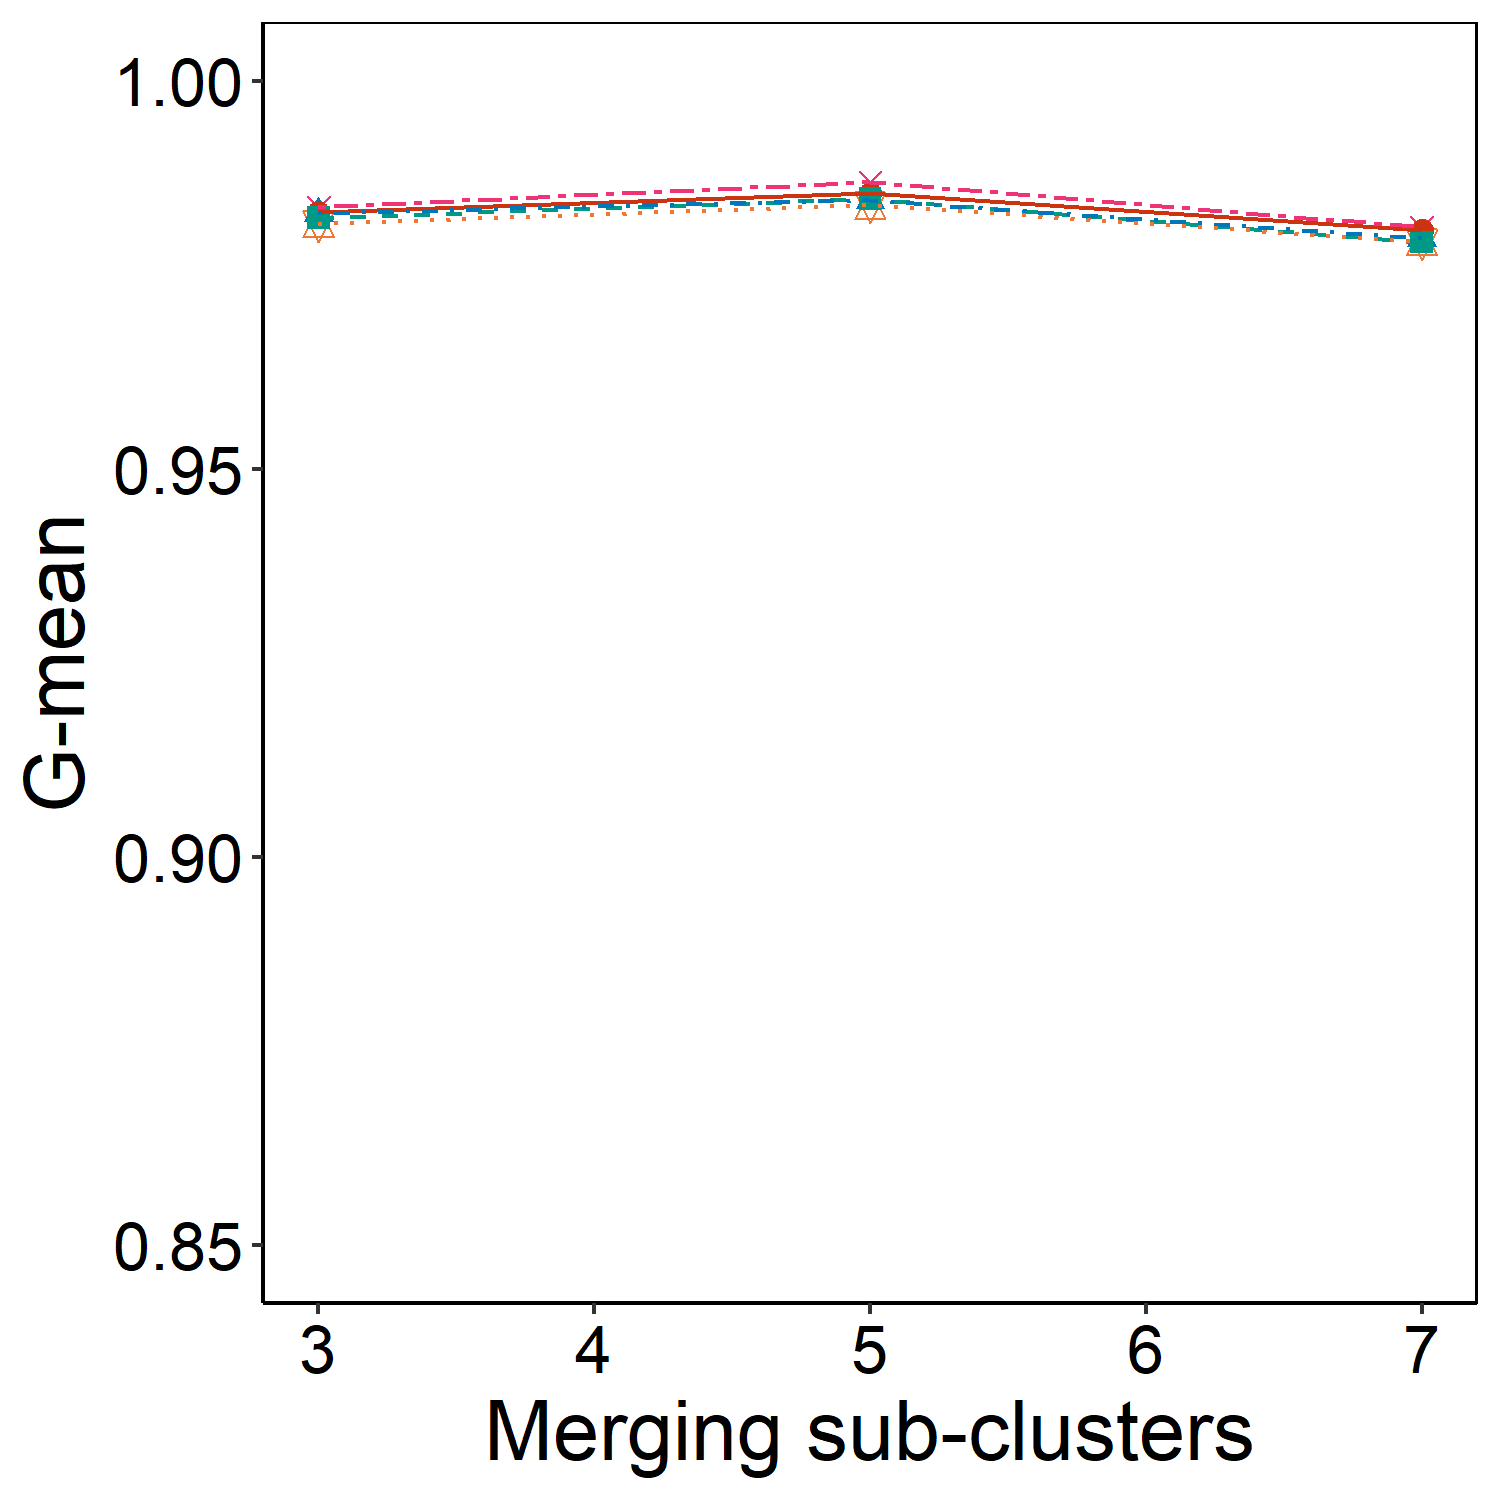
\includegraphics[width=4cm]{figures/join_plot_G-mean.png}}
    \caption{Porównanie jakości klasyfikacji przy zmianie liczby skupisk przykładów klasy mniejszościowej}\label{Figure:ChangeComposition}
\end{figure}

\noindent Podsumowując, wszystkie przedstawione algorytmy radziły sobie identycznie z problemem zmiany rozkładu klasy mniejszościowej. Jak można zauważyć na rysunku \ref{Figure:ChangeComposition} większa lub mniejsza liczba skupisk nie wpływała znacząco na jakość klasyfikacji zaprezentowanych modeli. Każdy z klasyfikatorów po wystąpieniu dryfu pojęć był w stanie przystosować się do zmian, które zaszły w strumieniu i powrócić na wysoki poziom jakości klasyfikacji.

\newpage

\noindent \textbf{Napływ przykładów określonego typu}\\

\noindent Ostatnim z analizowanych czynników trudności będzie napływ przykładów określonego typu. W ramach tej analizy rozważone zostaną przykłady o typie brzegowym (\english{borderline}) oraz rzadkim (\english{rare}).

\begin{table}[ht]
\centering\small%
\renewcommand{\arraystretch}{1.5} 
\begin{tabular}{l c c c c c c}
\toprule
Configuration & N & OB & UOB & OOB & NUOB & NOOB \\
\midrule
Safe stream & 0\% & 0.992 & 0.992 & 0.993 & 0.992 & 0.991 \\
Borderline[N] & 20\% & 0.978 & 0.978 & 0.978 & 0.979 & 0.969 \\
& 40\% & 0.974 & 0.974 & 0.974 & 0.976 & 0.965 \\
& 60\% & 0.972 & 0.971 & 0.972 & 0.973 & 0.963 \\
& 80\% & 0.971 & 0.970 & 0.971 & 0.972 & 0.961 \\
& 100\% & 0.969 & 0.968 & 0.969 & 0.970 & 0.959 \\
Rare[N] & 20\% & 0.935 & 0.935 & 0.935 & 0.935 & 0.934 \\
& 40\% & 0.865 & 0.865 & 0.865 & 0.865 & 0.866 \\
& 60\% & 0.779 & 0.779 & 0.779 & 0.779 & 0.800 \\
& 80\% & 0.684 & 0.680 & 0.690 & 0.677 & 0.752 \\
& 100\% & 0.677 & 0.668 & 0.689 & 0.661 & 0.692 \\
\bottomrule
\end{tabular}
\caption{Porównanie jakości klasyfikacji miary \textit{G-mean} w zależności od napływu przykładów określonego typu. Wartości w tabeli zostały wyznaczone jako średnia wszystkich wyników obliczonych podczas oceny odpowiedniego strumienia}\label{Tab:BorderlineRare}
\end{table}

\noindent Na podstawie przedstawionej tabeli \ref{Tab:BorderlineRare} można zauważyć, że porównywane klasyfikatory bardzo dobrze radzą sobie z napływem przykładów typu \textit{borderline}. Niestety widoczny jest znaczący spadek klasyfikacji w przypadku napływu przykładów typu \textit{Rare}. Identyczny efekt można zaobserwować przy zestawieniu wyników miary \textit{Recall}. Z zaprezentowanych rezultatów można wyciągnąć wniosek, że algorytm \textit{NOOB} radzi sobie trochę lepiej z rozpoznawaniem przykładów rzadkich aniżeli pozostałe algorytmy. Potwierdzenie tej obserwacji można zobaczyć na rysunku \ref{Figure:Rare80}.

\newpage

\begin{figure}[h]
    \centering
    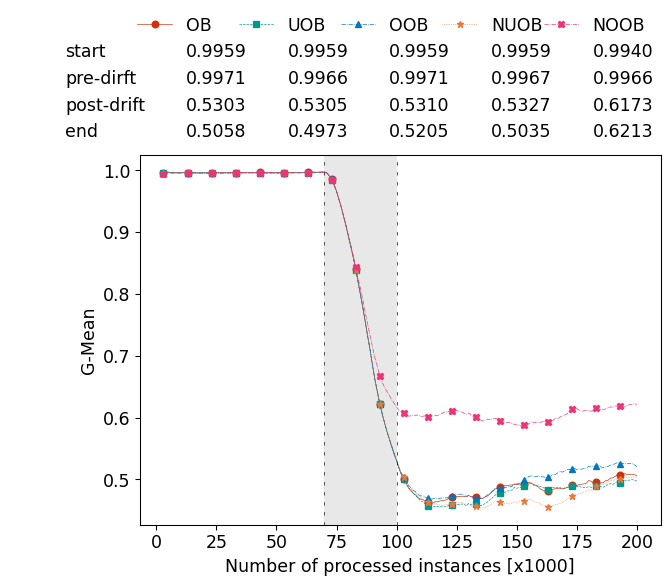
\includegraphics[width=12cm]{figures/rare80_gmean.png}
    \caption{Wykres liniowy miary \textit{G-mean} dla strumienia \textit{Rare80}}\label{Figure:Rare80}
\end{figure}

\begin{figure}[h]
    \centering
    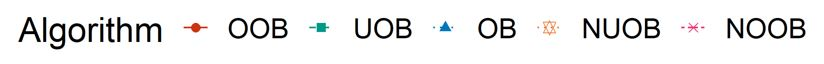
\includegraphics[width=7cm]{figures/algorithms_legend.JPG}
\end{figure}

\vspace{-1.2cm}

\begin{figure}[h]
    \centering
    \subfloat{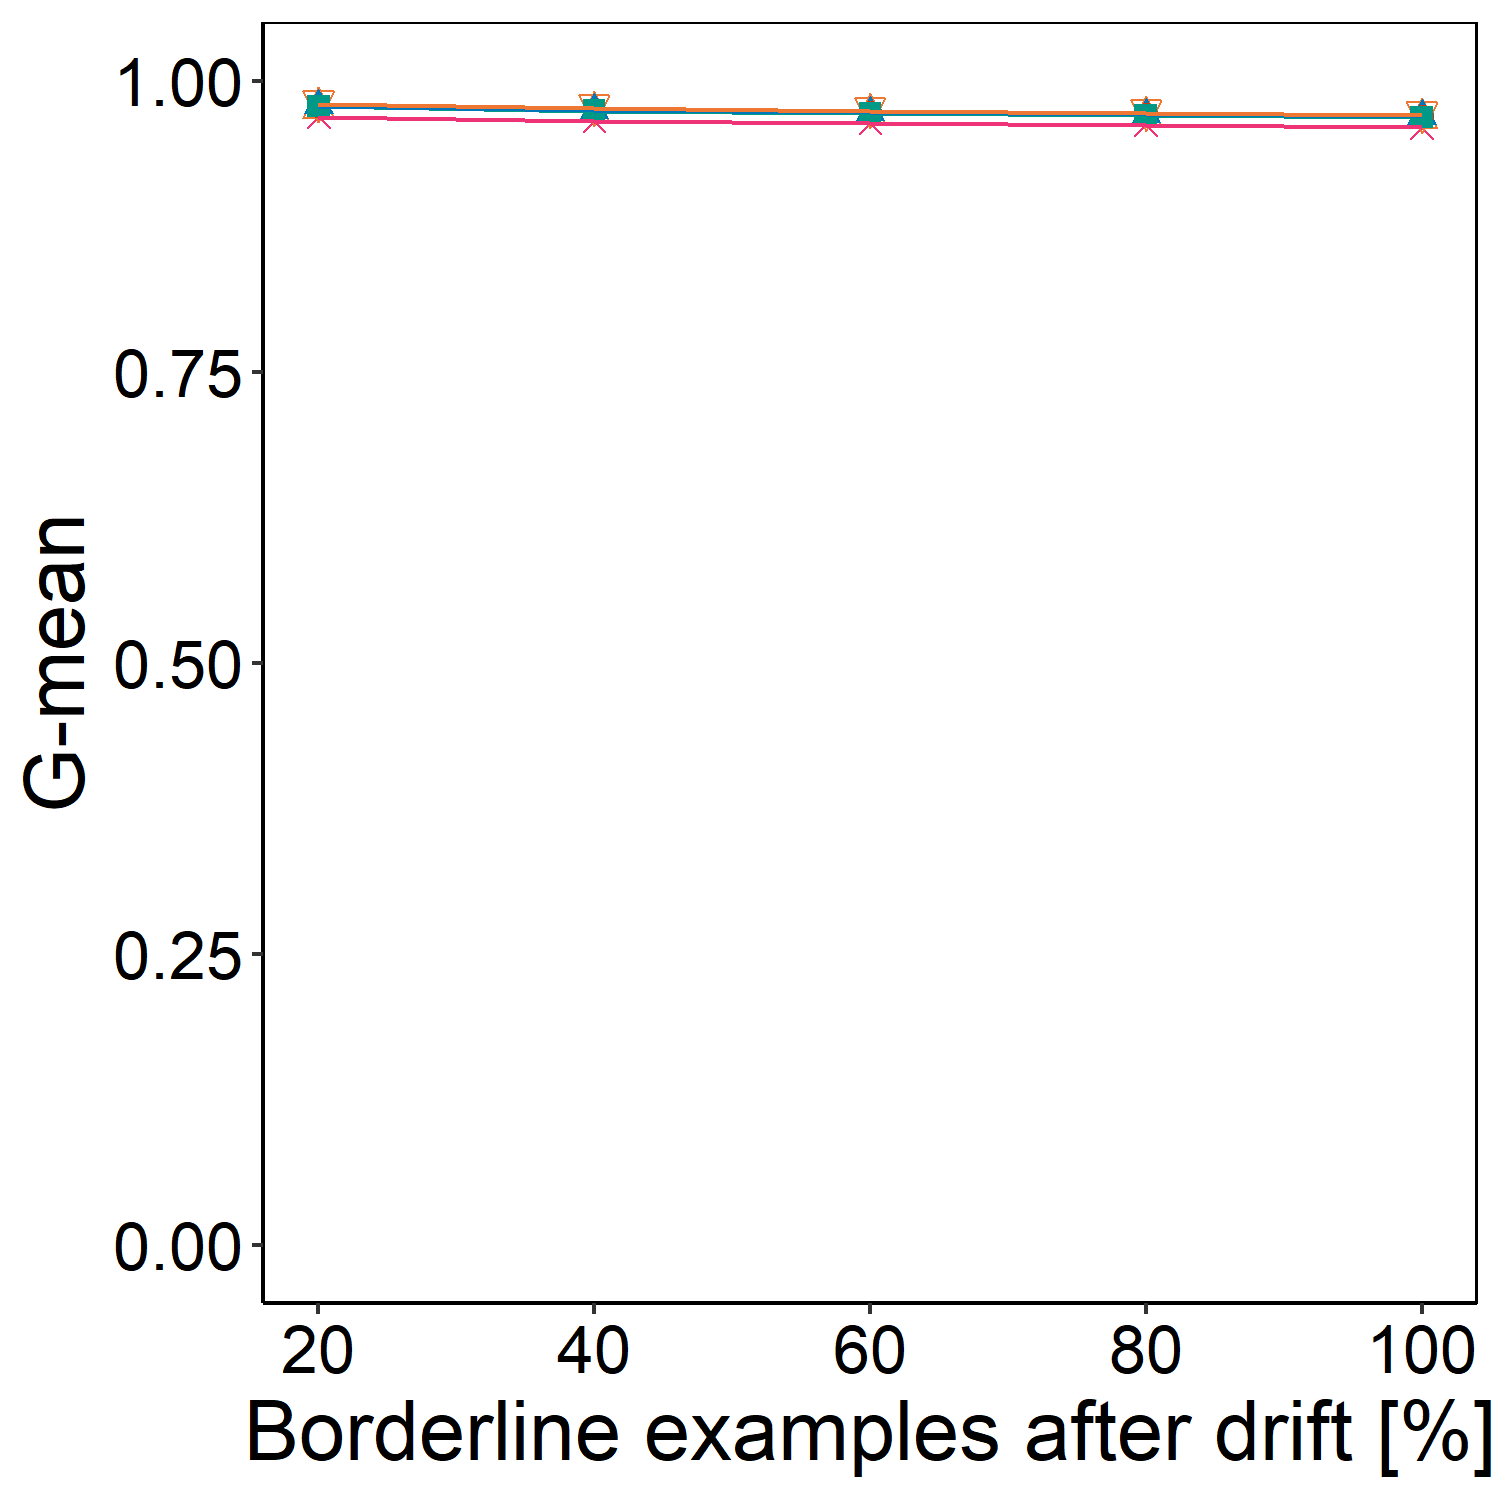
\includegraphics[width=7cm]{figures/borderline_plot_G-mean.png}}
    \qquad
    \subfloat{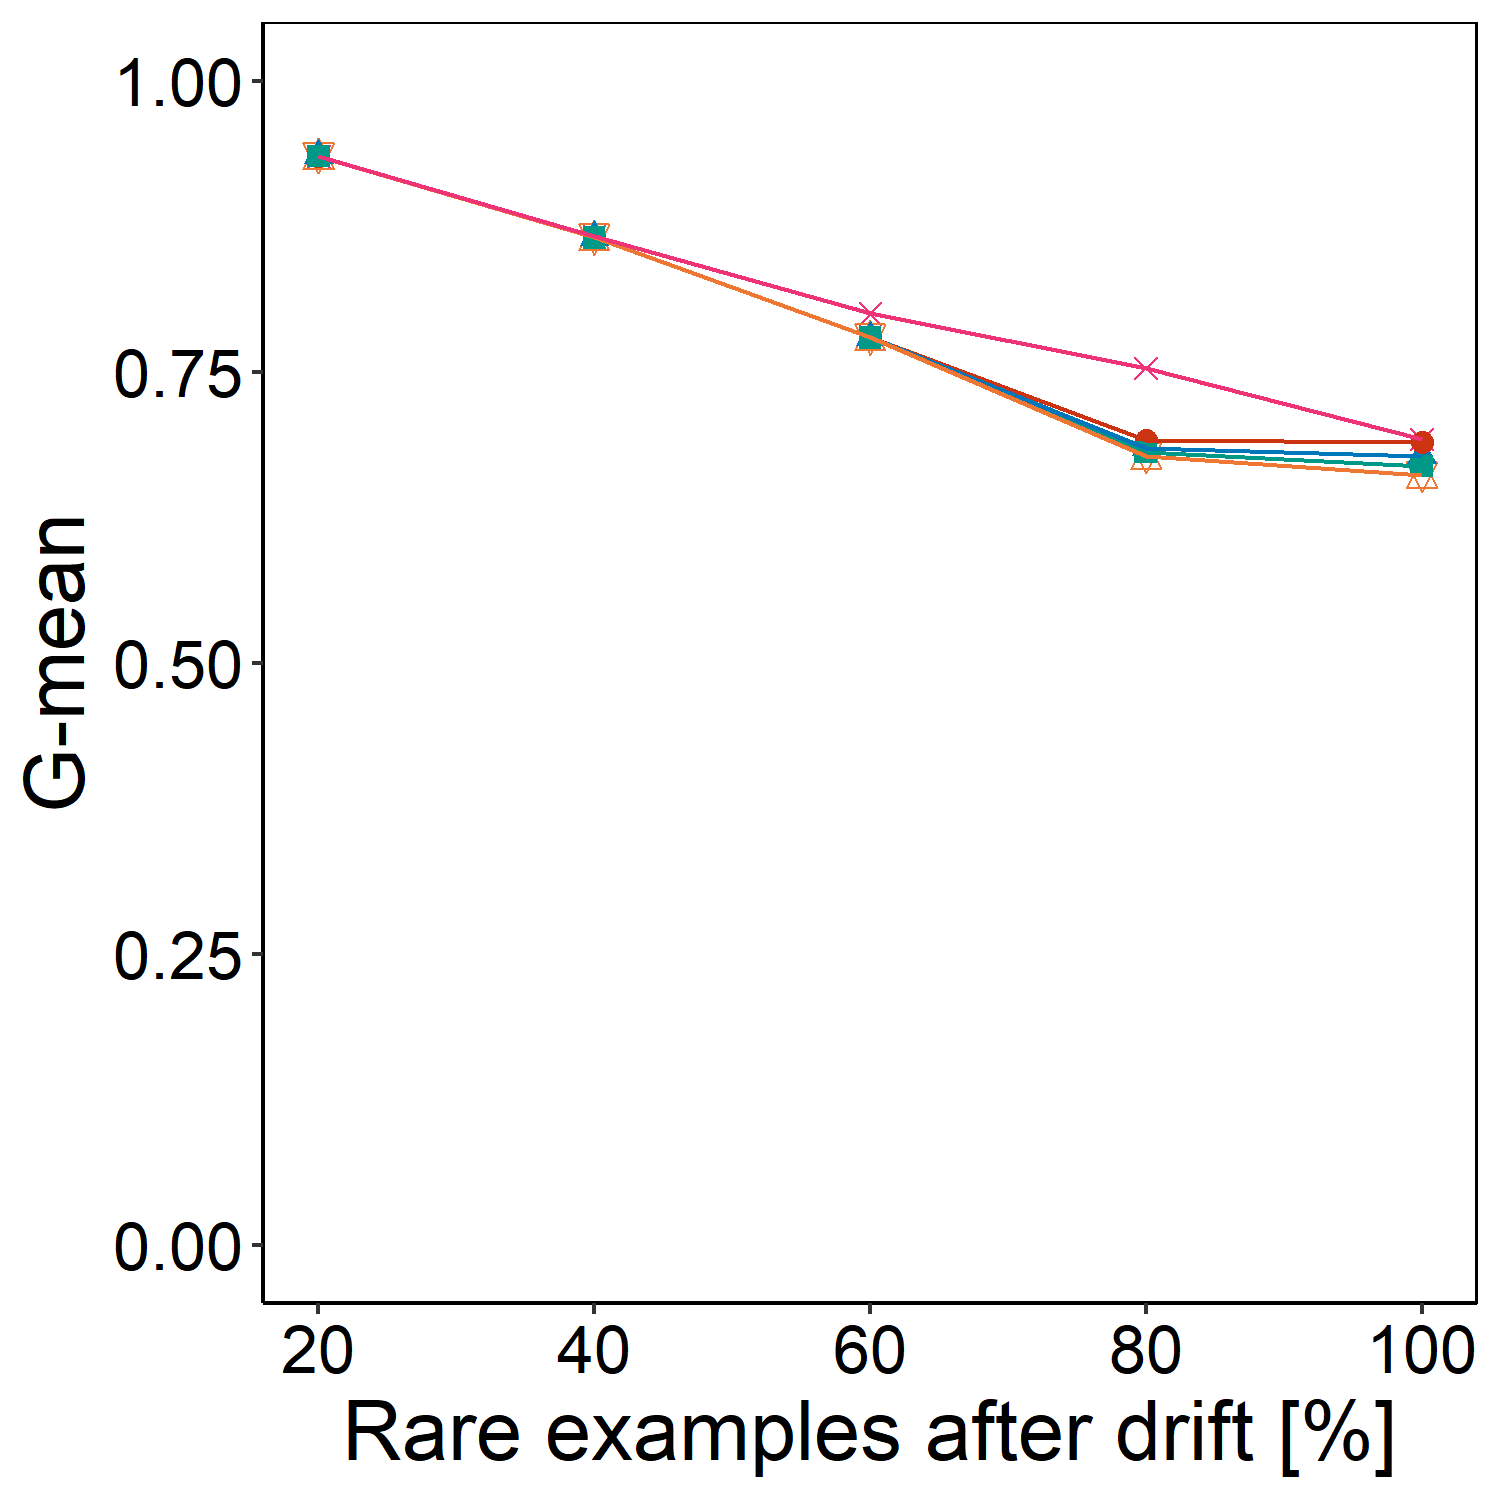
\includegraphics[width=7cm]{figures/rare_plot_G-mean.png}}
    \caption{Porównanie jakości klasyfikacji przy zmianie liczby przykładów określonego typu}\label{Figure:BorderlineRare}
\end{figure}

\noindent Podsumowując, wszystkie przedstawione algorytmy radzą sobie bardzo dobrze ze wzrostem przykładów typu \textit{Borderline}. Niestety w przypadku wzrostu elementów typu \textit{Rare} widoczny jest znaczący spadek jakości klasyfikacji. Jedynym wyróżniającym się algorytmem, który radził sobie lepiej od pozostałych z rozpoznawaniem przykładów rzadkich, był algorytm \textit{NOOB}, jednak nawet ten klasyfikator nie dał rady odpowiednio dostosować się do zmian i powrócić na swój początkowy poziom jakości klasyfikacji przed wystąpieniem dryfu.

\noindent \textbf{Porównanie statystyczne klasyfikatorów}\\

\noindent W ramach ostatniego punktu analizy klasyfikatorów pod kątem strumieni danych z jednym czynnikiem trudności, przeprowadzony zostanie test statystyczny rang Friedman'a, którego kontynuacją będzie przeprowadzenie testu Nemenyi jako testu \textit{post hoc}. Testy zostały przeprowadzone na poziomie istotności $\alpha$ = 0.05.

\begin{table}[ht]
\centering\small%
\setlength{\tabcolsep}{10pt} 
\renewcommand{\arraystretch}{1.5} 
\begin{tabular}{l l c c c c c c}
\toprule
Data stream set & Metric & OB & UOB & OOB & NUOB & NOOB & CD \\
\midrule
Static imbalance & G-mean & 3.82 & \textbf{2.00} & \textbf{2.29} & \textbf{3.29} & 3.59 & 1.51 \\
Class ratio changes & & 4.55 & \textbf{1.59} & 2.61 & 3.14 & 3.11 & 0.77 \\
Sub-cluster merge & & \textbf{2.67} & \textbf{3.83} & \textbf{2.33} & \textbf{3.17} & \textbf{3.00} & 2.68 \\
Sub-cluster move & & \textbf{2.67} & 4.83 & \textbf{1.33} & 4.17 & \textbf{2.00} & 2.68 \\
Sub-cluster split & & \textbf{2.17} & \textbf{4.50} & \textbf{2.17} & \textbf{2.00} & \textbf{4.17} & 2.68 \\
Borderline examples & & \textbf{1.70} & 4.00 & \textbf{2.40} & \textbf{2.60} & 4.30 & 2.01 \\
Rare examples & & \textbf{2.80} & 4.20 & \textbf{1.90} & 4.00 & \textbf{2.10} & 2.01 \\
Static imbalance & Recall & 4.35 & \textbf{2.41} & 3.35 & \textbf{1.00} & 3.88 & 1.51 \\
Class ratio changes & & 4.88 & 2.17 & 3.59 & \textbf{1.00} & 3.36 & 0.77 \\
Sub-cluster merge & & \textbf{2.67} & \textbf{3.67} & \textbf{2.67} & \textbf{1.00} & 5.00 & 2.68 \\
Sub-cluster move & & \textbf{3.17} & \textbf{3.17} & \textbf{2.67} & \textbf{1.00} & 5.00 & 2.68 \\
Sub-cluster split & & \textbf{2.50} & \textbf{2.50} & 4.00 & \textbf{1.00} & 5.00 & 2.68 \\
Borderline examples & & \textbf{2.70} & 3.80 & \textbf{2.50} & \textbf{1.00} & 5.00 & 2.01 \\
Rare examples & & \textbf{3.90} & \textbf{3.80} & \textbf{2.80} & \textbf{2.10} & \textbf{2.40} & 2.01 \\
\bottomrule
\end{tabular}
\caption{Wyniki przeprowadzonych testów statystycznych dla pojedynczych czynników trudności}\label{Tab:SingleDriftFriedman}
\end{table}

\noindent W tabeli \ref{Tab:SingleDriftFriedman} zestawione zostały wyniki przeprowadzonych testów statystycznych. Interpretacja wyników otrzymanych w tabeli jest następująca - im mniejsza wartość rangi dla danego algorytmu tym lepsze rezultaty osiągało dane podejście. Pogrubione zostały najlepsze wyniki dla określonych zbiorów danych oraz wyniki, które okazały się nie być statystycznie różne od najlepszego wyniku. Kolumna \textit{CD} oznacza odległość krytyczną (\english{critical distance}), na podstawie której to wartości można określić czy dwa otrzymane wyniki są od siebie statystycznie różne czy nie (na zadanym poziomie istotności). Na podstawie otrzymanych rezultatów możliwe jest określenie rankingu algorytmów pod kątem danej miary:

\begin{itemize}
    \item \textit{G-mean} - OOB $\succ$ OB $\succ$ UOB, NUOB, NOOB
    \item \textit{Recall} - NUOB $\succ$ OB, UOB $\succ$ OOB $\succ$ NOOB
\end{itemize}

\noindent Najlepszym algorytmem pod kątem miary \textit{G-mean}, dla strumieni danych charakteryzujących się występowaniem jednego czynnika trudności, okazał się algorytm \textit{OOB}, co jest niekorzystnym wynikiem, gdyż pokazuje to, że zaproponowane rozszerzenia nie radzą sobie najlepiej. Obserwacja ta pozostawia pole do poprawy oraz dalszej analizy względem zaproponowanych algorytmów. Pod kątem miary \textit{Recall} najlepszy był nowo zaprezentowany algorytm \textit{NUOB}.

\subsection{Data streams with pairs of factors}

\noindent W niniejszej sekcji zaprezentowane algorytmy zostaną przetestowane pod kątem jakości klasyfikacji na strumieniach danych z dwoma czynnikami trudności (\english{pairs of factors}). Jak się okazało, na podstawie wyników poprzedniej sekcji, najbardziej wymagającym czynnikiem, z którym algorytmy miały największe problemy, był napływ przykładów typu \textit{Rare}. Bardzo podobnie sytuacja wygląda w przypadku analizy par czynników, które mogą wystąpić w strumieniu. Jeżeli jednym z tych czynników jest napływ rzadkich przykładów to jakość klasyfikacji jest zdecydowanie niższa aniżeli gdy dokonujemy analizy strumienia zawierającego inne własności. Odwzorowanie tej sytuacji można zobaczyć na rysunkach \ref{Figure:Split5Pairs} oraz \ref{Figure:PairsFactors}.

\begin{figure}[h]
    \centering
    \subfloat{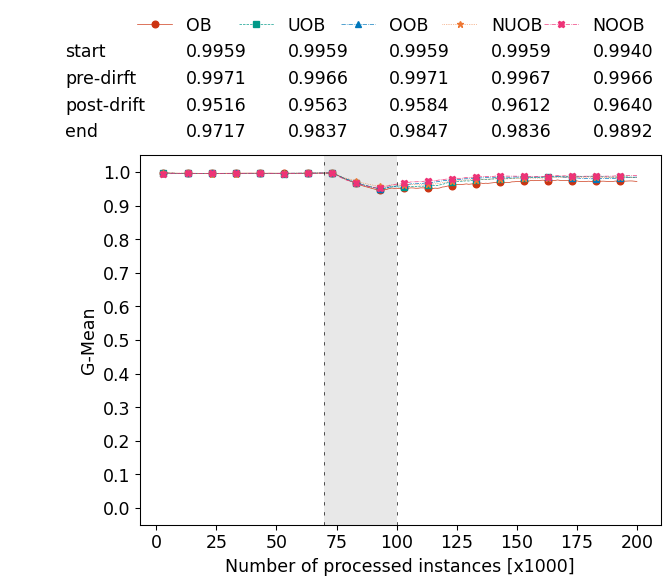
\includegraphics[width=7cm]{figures/split5im10_gmean.png}}
    \qquad
    \subfloat{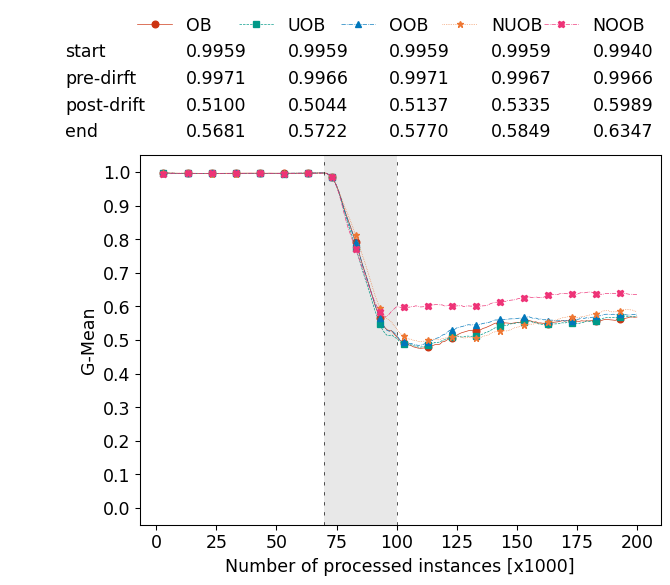
\includegraphics[width=7cm]{figures/split5rare80_gmean.png}}
    \caption{Wykresy liniowe miary \textit{G-mean} dla strumieni \textit{Split5+Im10} (po lewej) oraz \textit{Split5+Rare80} (po prawej)}\label{Figure:Split5Pairs}
\end{figure}

\begin{figure}[h]
    \centering
    \subfloat{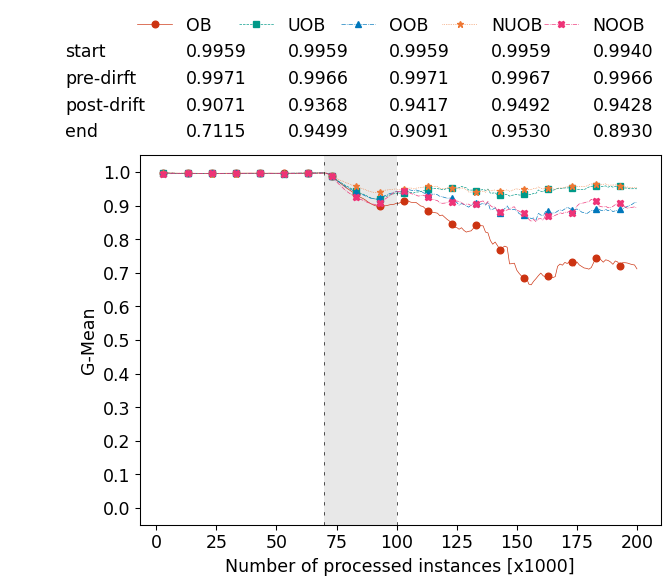
\includegraphics[width=7cm]{figures/im1borderline80_gmean.png}}
    \qquad
    \subfloat{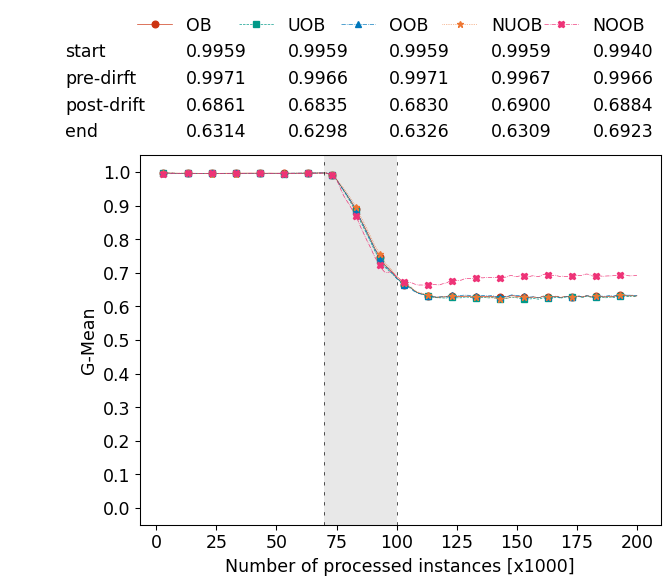
\includegraphics[width=7cm]{figures/split5rare60_gmean.png}}
    \caption{Wykresy liniowe miary \textit{G-mean} dla strumieni \textit{Im1+Borderline80} (po lewej) oraz \textit{Split5+Rare60} (po prawej)}\label{Figure:PairsFactors}
\end{figure}

\noindent Podobnie, jak to można było zauważyć we wcześniejszej sekcji, algorytm NOOB radzi sobie trochę lepiej z rozpoznawaniem przykładów rzadkich w porównaniu do innych algorytmów. Aby potwierdzić tę tezę na innych scenariuszach, zdecydowano się zestawić wyniki wszystkich algorytmów na najbardziej wymagających strumieniach danych. Otrzymane wyniki widoczne są na rysunku \ref{Figure:PairsComparison}.

\begin{figure}[h]
    \centering
    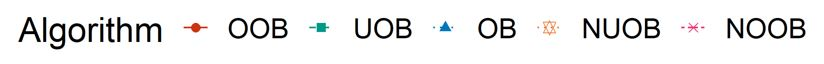
\includegraphics[width=7cm]{figures/algorithms_legend.JPG}
\end{figure}

\vspace{-1.2cm}

\begin{figure}[h]
    \centering
    \subfloat{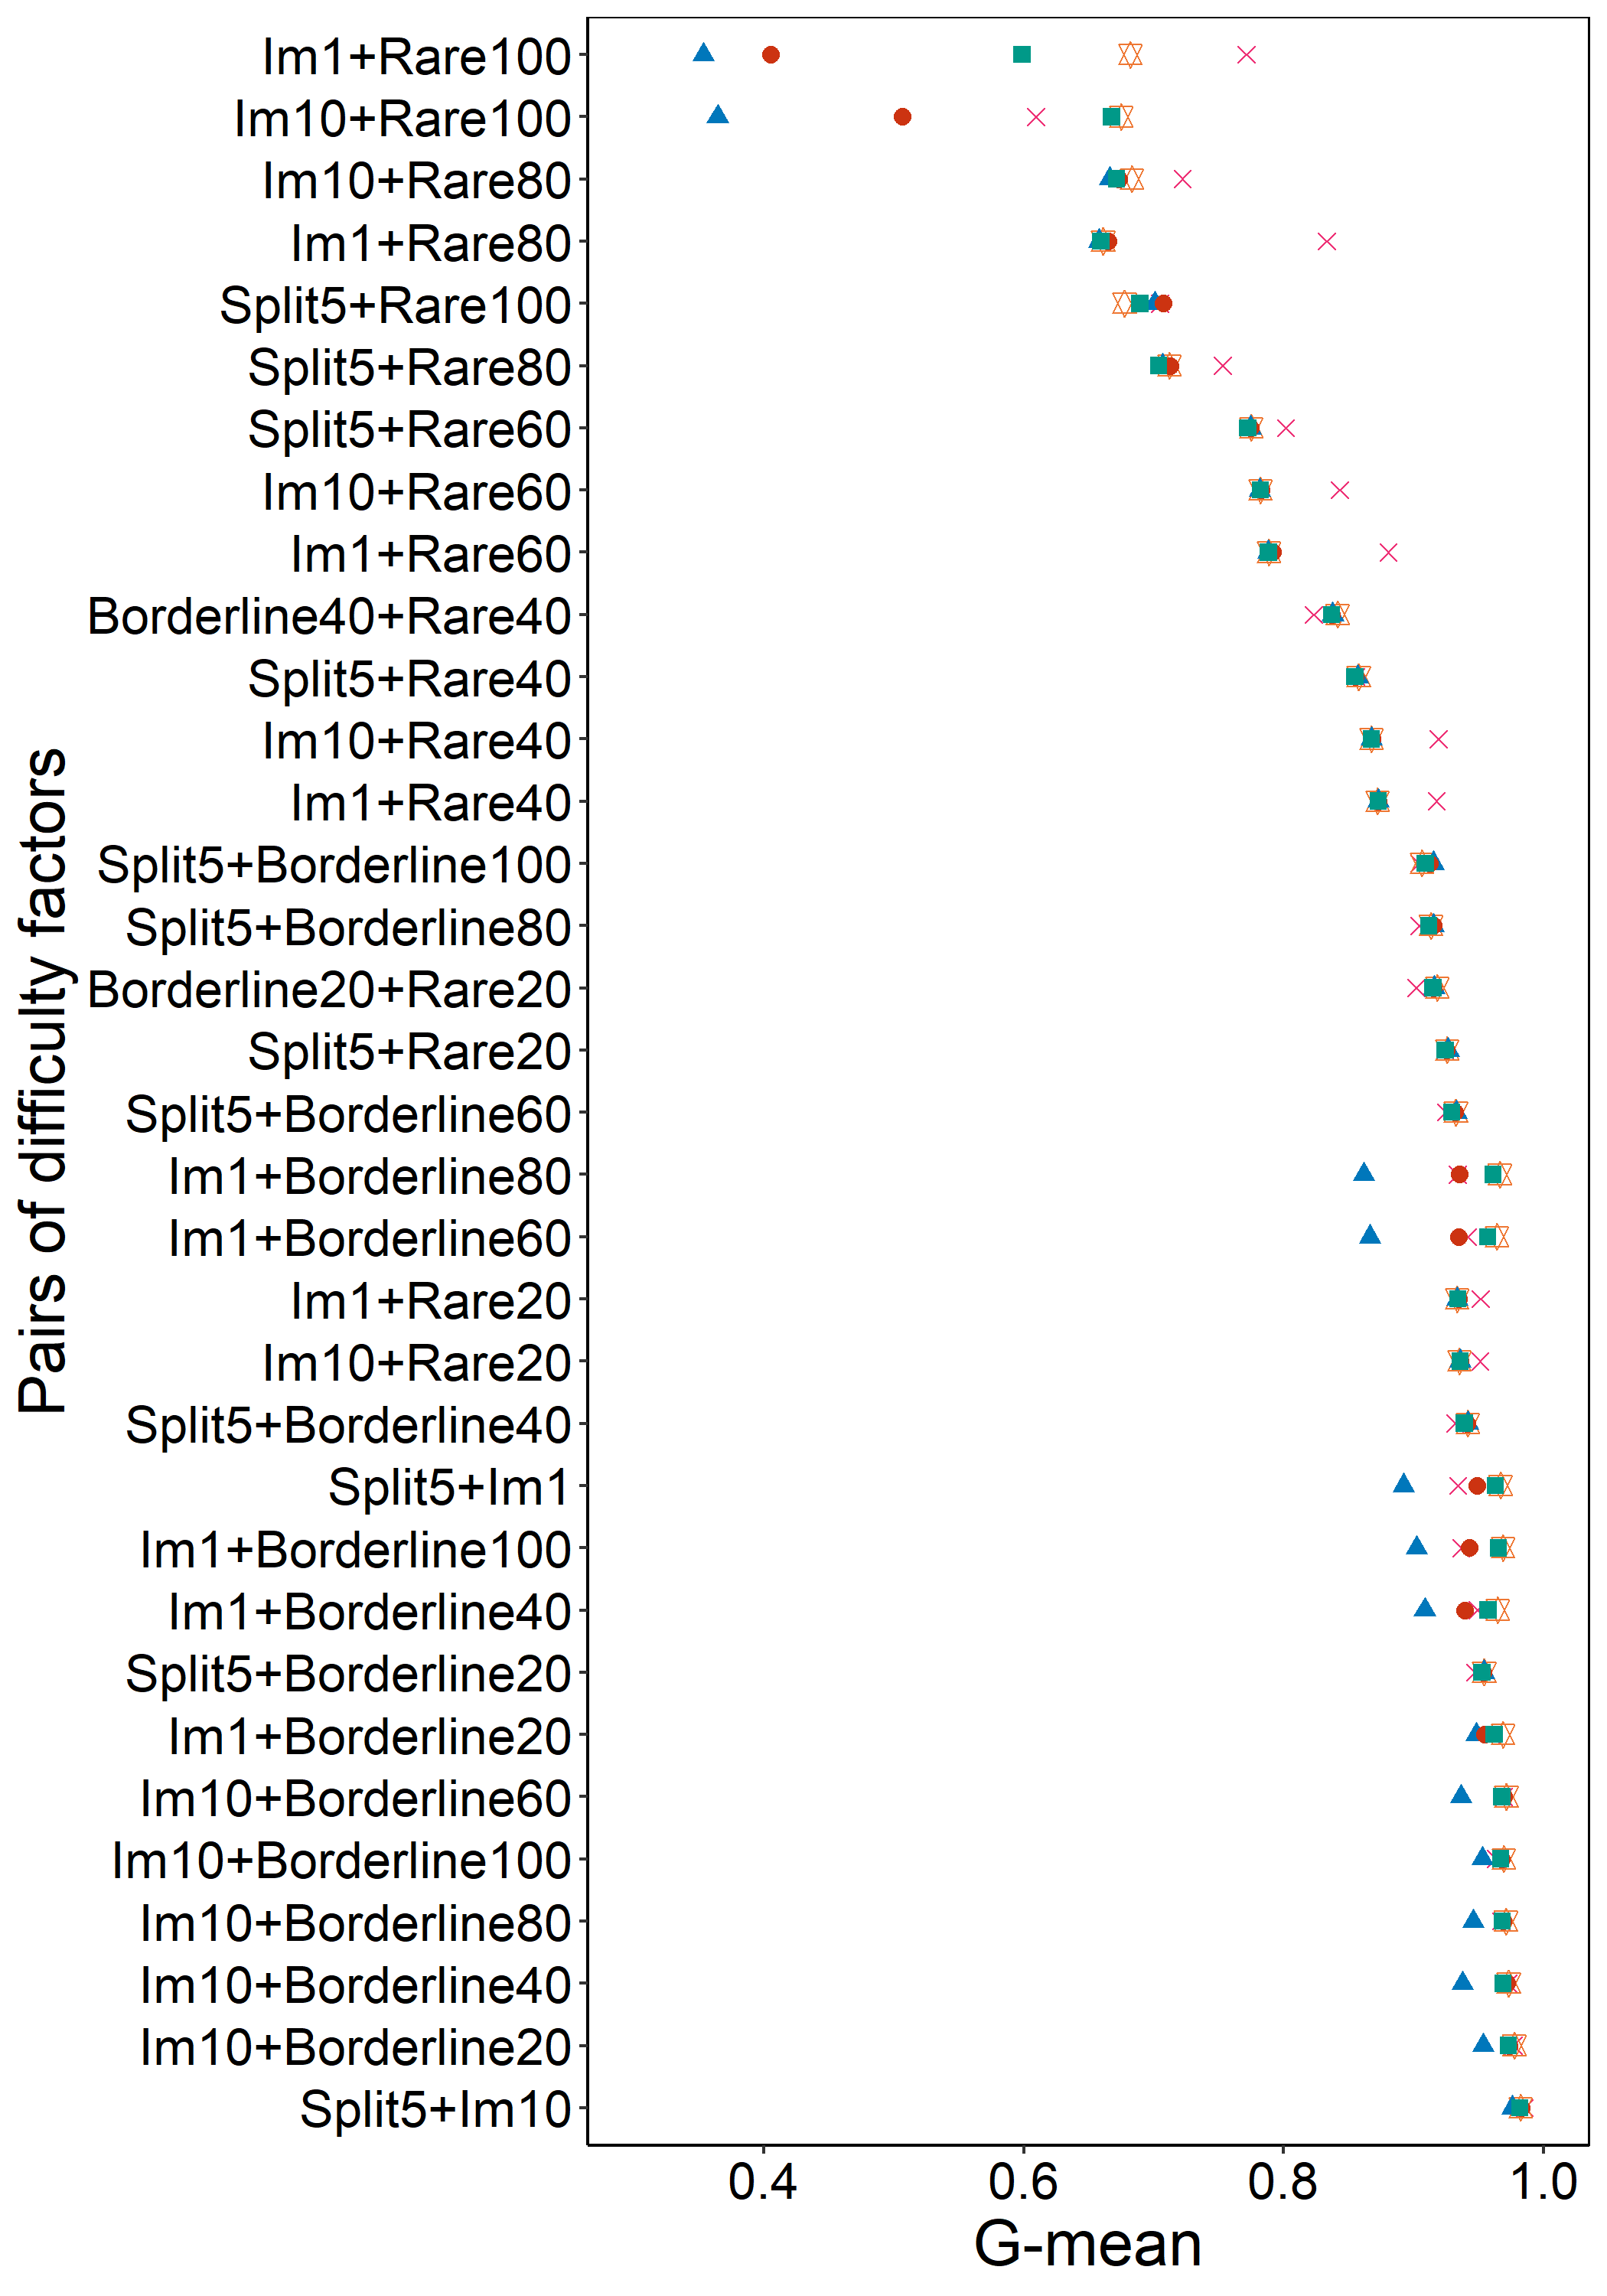
\includegraphics[width=7cm]{figures/pair_plot_G-mean.png}}
    \qquad
    \subfloat{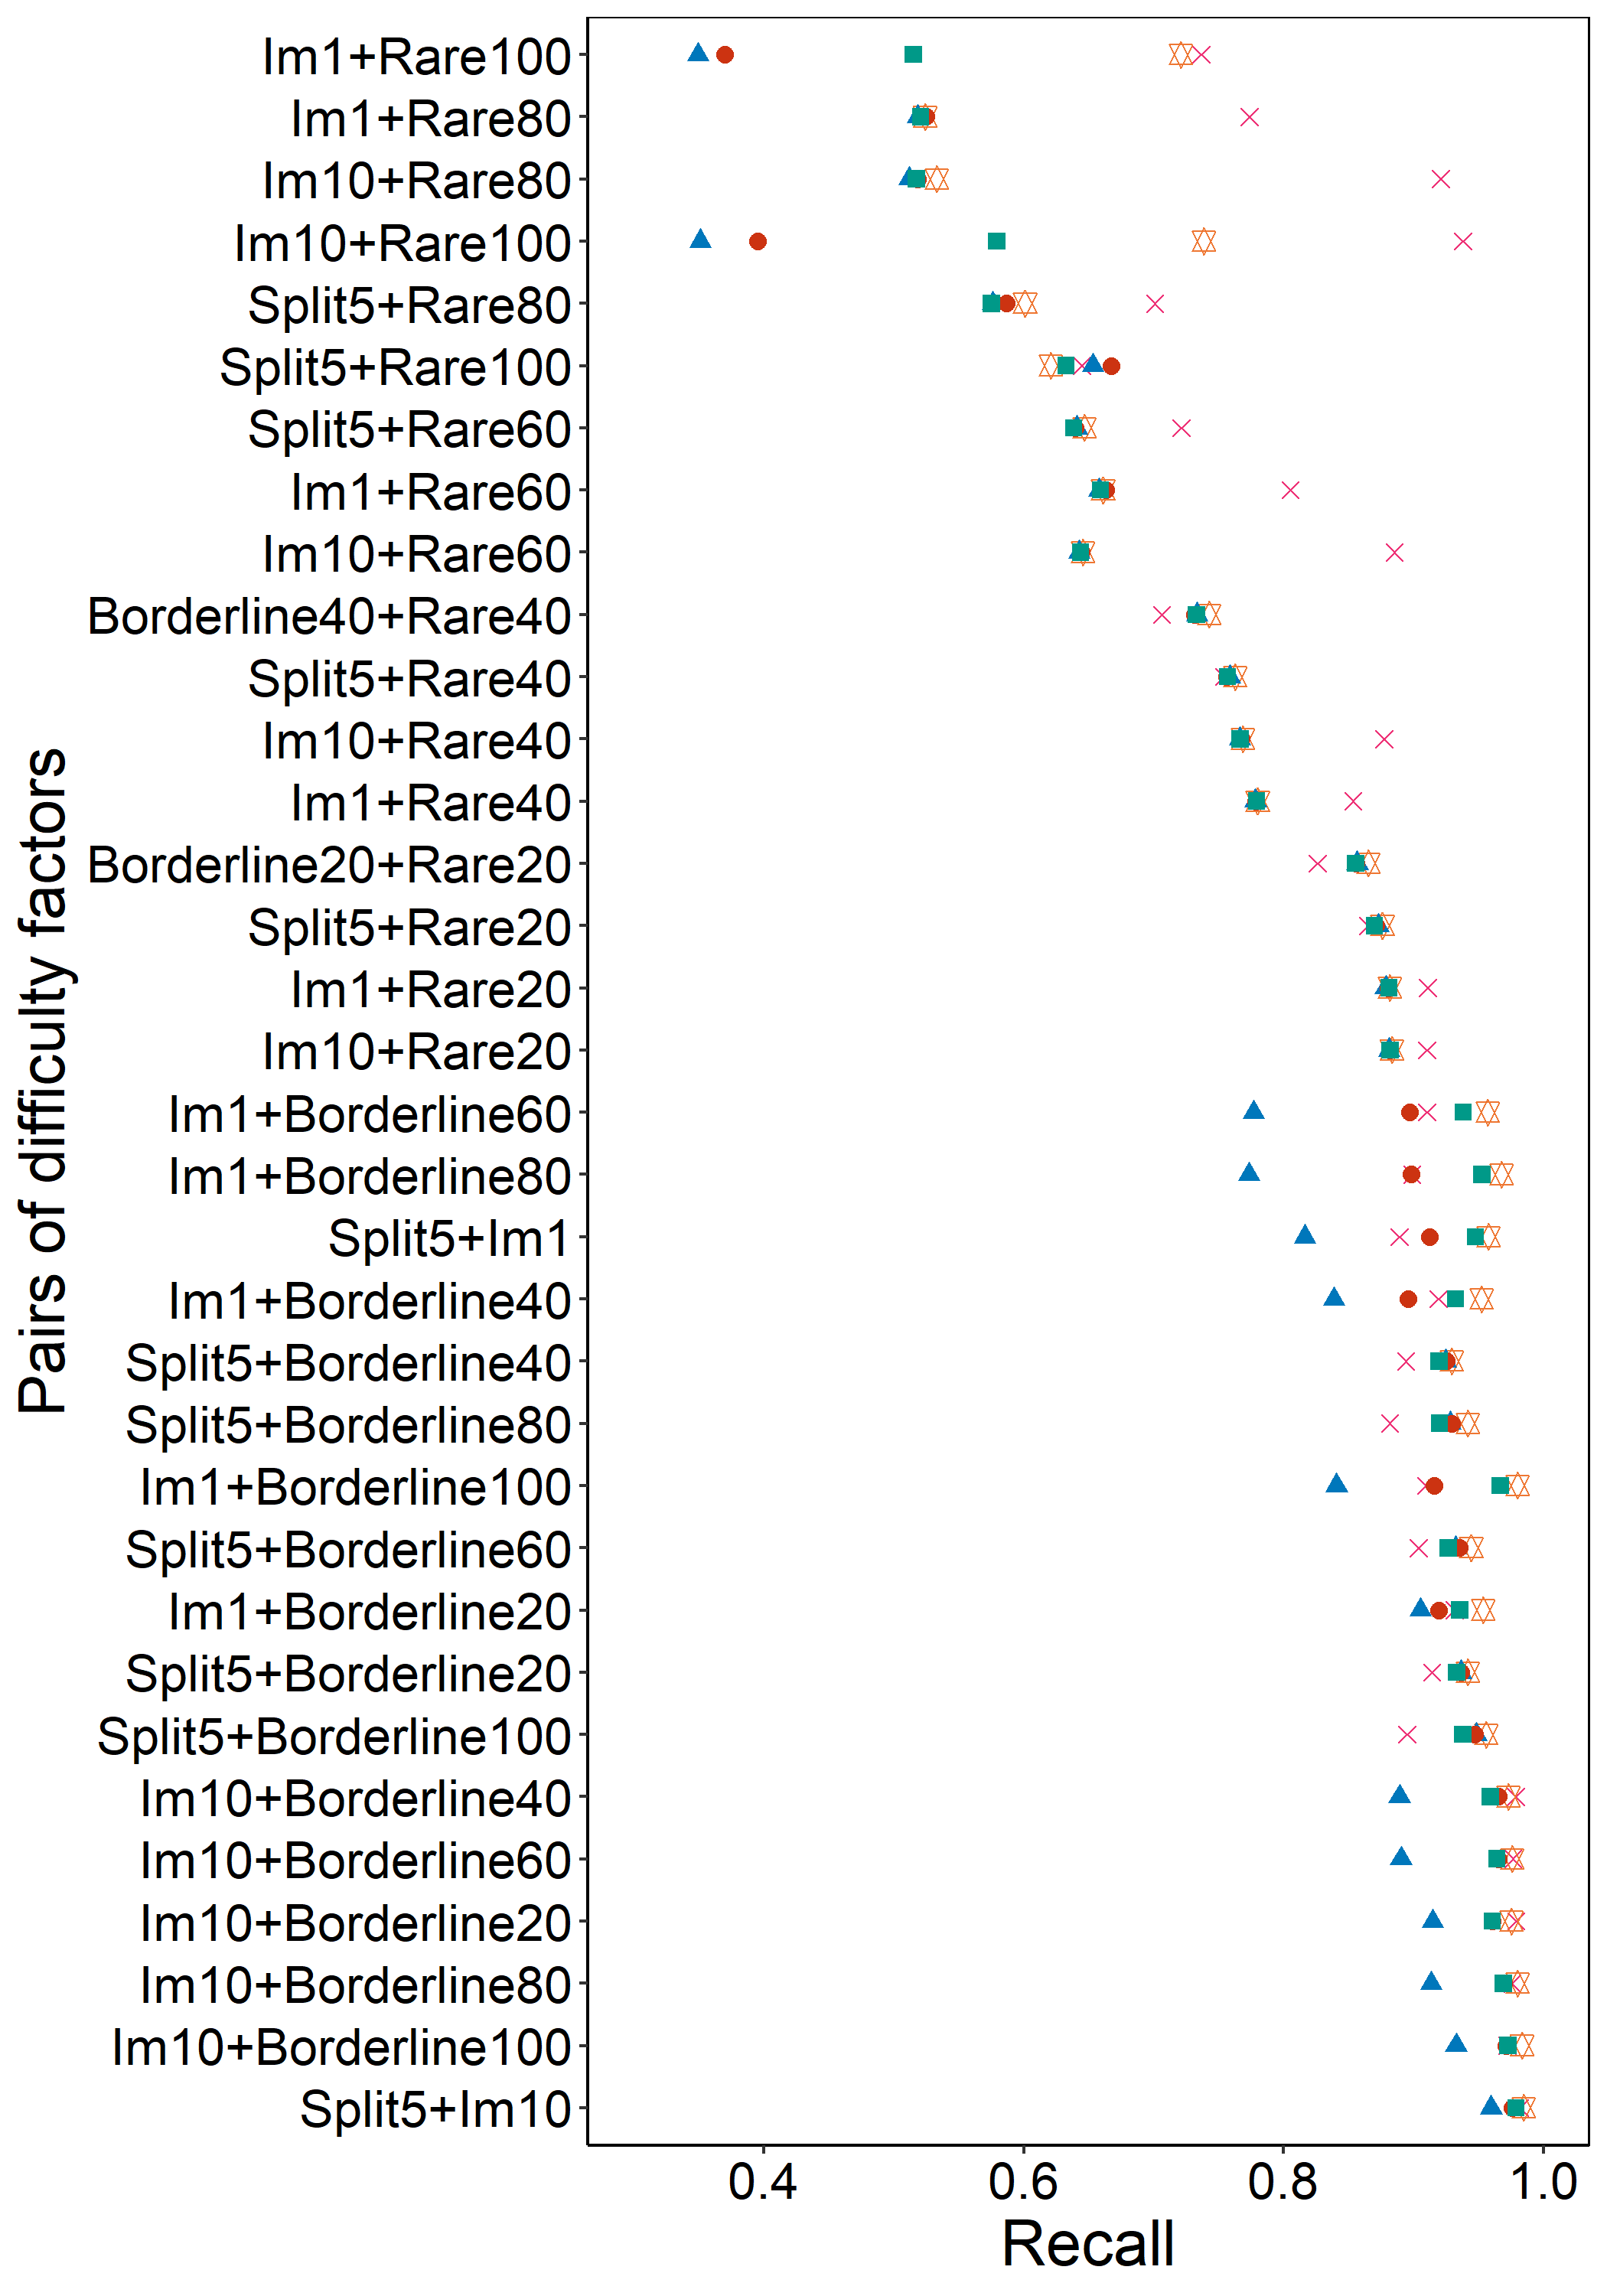
\includegraphics[width=7cm]{figures/pair_plot_Recall.png}}
    \caption{Porównanie jakości klasyfikacji na najbardziej wymagających strumieniach danych zawierających dwa czynniki trudności}\label{Figure:PairsComparison}
\end{figure}

\noindent Jak można zauważyć na ilustracji \ref{Figure:PairsComparison} algorytm \textit{NOOB} radzi sobie zdecydowanie lepiej od pozostałych algorytmów na najbardziej wymagających strumieniach danych. Przykładowo dla strumienia \textit{Im1+Rare80} wartość miary \textit{G-mean} dla algorytmu \textit{NOOB} wynosi około 0.8, podczas gdy dla pozostałych algorytmów jest to wartość około 0.65. Podobne rezultaty można zaobserwować dla tego samego strumienia dla miary \textit{Recall}. Dla podejścia \textit{NOOB} jest to wartość około 0.75, a dla pozostałych algorytmów około 0.5. Analogiczną sytuację można zaobserwować na strumieniu \textit{Im10+Rare60} lub \textit{Im10+Rare40}. Należy także zwrócić uwagę na obserwację dotyczącą tego, że algorytmy \textit{OB} oraz \textit{OOB} kompletnie nie radzą sobie z klasyfikacją trudnych strumieni danych - na strumieniu \textit{Im1+Rare100} wartość miar \textit{G-mean} oraz \textit{Recall} oscyluje koło wartości 0.4.

Podobnie jak w poprzedniej sekcji przeprowadzono porównanie statystyczne klasyfikatorów z wykorzystaniem testu statystycznego rang Friedman'a oraz testu Nemenyi na poziomie istotności $\alpha$ = 0.05.

\newpage

\begin{table}[ht]
\centering\small%
\setlength{\tabcolsep}{10pt} 
\renewcommand{\arraystretch}{1.5} 
\begin{tabular}{l l c c c c c c}
\toprule
Data stream set & Metric & OB & UOB & OOB & NUOB & NOOB & CD \\
\midrule
Imbalance + Move & G-mean & 5.00 & \textbf{2.33} & \textbf{2.75} & \textbf{2.67} & \textbf{2.25} & 1.82 \\
Imbalance + Merge  & & 5.00 & \textbf{1.75} & \textbf{3.08} & \textbf{2.25} & \textbf{2.92} & 1.82 \\
Imbalance + Split  & & 5.00 & \textbf{2.11} & 3.50 & \textbf{2.00} & \textbf{2.39} & 1.47 \\
Imbalance + Borderline  & & 5.00 & \textbf{2.42} & 3.38 & \textbf{1.68} & \textbf{2.52} & 0.97 \\
Imbalance + Rare  & & 4.85 & 2.88 & 3.10 & 2.95 & \textbf{1.23} & 0.97 \\
Split + Borderline  & & 4.36 & \textbf{2.44} & 3.22 & \textbf{2.14} & \textbf{2.84} & 0.87 \\
Split + Rare  & & 4.54 & 2.94 & 3.24 & 2.76 & \textbf{1.52} & 0.87 \\
Imbalance + Move & Recall & 5.00 & \textbf{2.17} & 3.83 & \textbf{1.33} & \textbf{2.67} & 1.82 \\
Imbalance + Merge  & & 5.00 & \textbf{2.00} & 3.83 & \textbf{1.42} & \textbf{2.75} & 1.82 \\
Imbalance + Split  & & 5.00 & \textbf{2.06} & 3.83 & \textbf{1.33} & \textbf{2.78} & 1.47 \\
Imbalance + Borderline  & & 5.00 & 2.52 & 3.88 & \textbf{1.35} & \textbf{2.25} & 0.97 \\
Imbalance + Rare  & & 5.00 & 2.73 & 3.83 & \textbf{2.10} & \textbf{1.35} & 0.97 \\
Split + Borderline  & & 4.52 & 2.60 & 3.68 & \textbf{1.60} & 2.60 & 0.87 \\
Split + Rare  & & 4.50 & \textbf{2.72} & 3.76 & \textbf{2.16} & \textbf{1.86} & 0.87 \\
\bottomrule
\end{tabular}
\caption{Wyniki przeprowadzonych testów statystycznych dla par czynników trudności}\label{Tab:DoubleDriftFriedman}
\end{table}

\noindent W tabeli \ref{Tab:DoubleDriftFriedman} zestawione zostały wyniki przeprowadzonych testów statystycznych. Interpretacja wyników otrzymanych w tabeli jest następująca - im mniejsza wartość rangi dla danego algorytmu tym lepsze rezultaty osiągało dane podejście. Pogrubione zostały najlepsze wyniki dla określonych zbiorów danych oraz wyniki, które okazały się nie być statystycznie różne od najlepszego wyniku. Na podstawie otrzymanych rezultatów możliwe jest określenie rankingu algorytmów pod kątem danej miary:

\begin{itemize}
    \item \textit{G-mean} - NOOB $\succ$ UOB, NUOB $\succ$ OOB $\succ$ OB
    \item \textit{Recall} - NUOB $\succ$ NOOB $\succ$ UOB $\succ$ OB, OOB
\end{itemize}

\noindent Najlepszym algorytmem pod kątem miary \textit{G-mean}, dla strumieni charakteryzujących się występowaniem par czynników trudności, okazał się \textit{NOOB}. Pod kątem miary \textit{Recall} ponownie najlepszy był algorytm \textit{NUOB}. Warto odnotować, że algorytmy \textit{OB} oraz \textit{OOB} osiągnęły słabe wyniki w porównaniu do innych algorytmów, co sugeruje, że niekoniecznie radzą sobie ze złożonymi instancjami strumieni danych.

\subsection{Complex scenarios}

\noindent W ramach tej części zaprezentowane algorytmy zostaną przetestowane pod kątem jakości klasyfikacji na strumieniach danych z wieloma czynnikami trudności (\english{complex scenarios}). Podobnie jak to było przy ocenie strumieni z dwoma czynnikami trudności, tak tutaj największy wpływ na jakość klasyfikacji ma napływ elementów rzadkich. Z takimi scenariuszami radzi sobie najlepiej algorytm \textit{NOOB}, czego odzwierciedlenie można zobaczyć na rysunku \ref{Figure:ComlexScenario}.

\newpage

\begin{figure}[h]
    \centering
    \subfloat{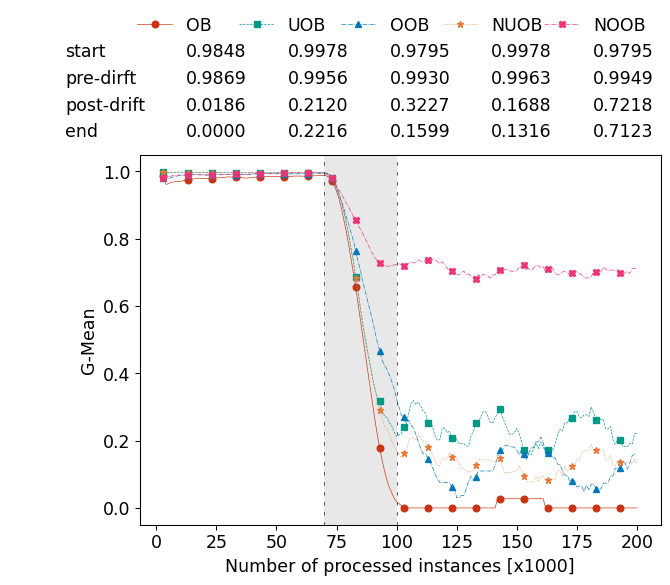
\includegraphics[width=7cm]{figures/complex_scenario_gmean.png}}
    \qquad
    \subfloat{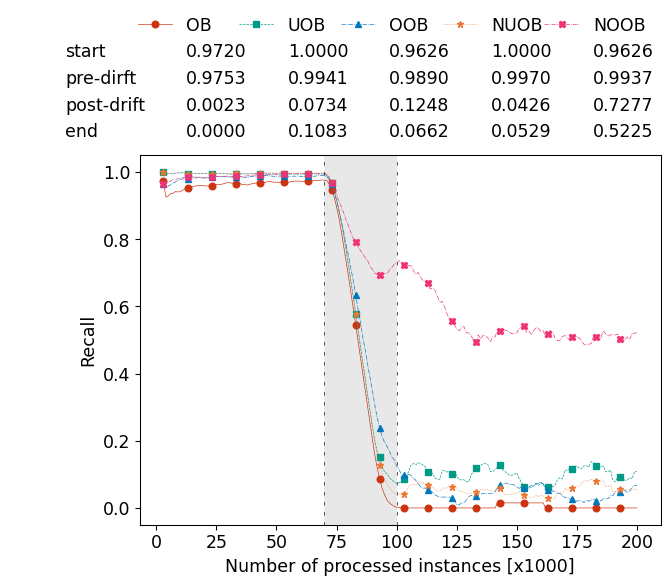
\includegraphics[width=7cm]{figures/complex_scenario_recall.png}}
    \caption{Wykresy liniowe miar \textit{G-mean} oraz \textit{Recall} dla strumienia \textit{StaticIm10+Split5+Im1+Rare80}}\label{Figure:ComlexScenario}
\end{figure}

\noindent W celach porównawczych dokonano zestawienia wyników algorytmów na strumieniach danych, które najbardziej wpływają na spadek jakości klasyfikacji. Otrzymane wyniki widoczne są na rysunku \ref{Figure:ComplexComparison}.

\begin{figure}[h]
    \centering
    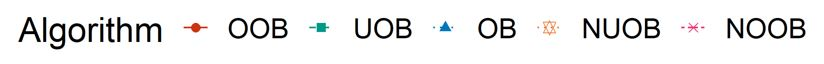
\includegraphics[width=7cm]{figures/algorithms_legend.JPG}
\end{figure}

\vspace{-1.2cm}

\begin{figure}[h]
    \centering
    \subfloat{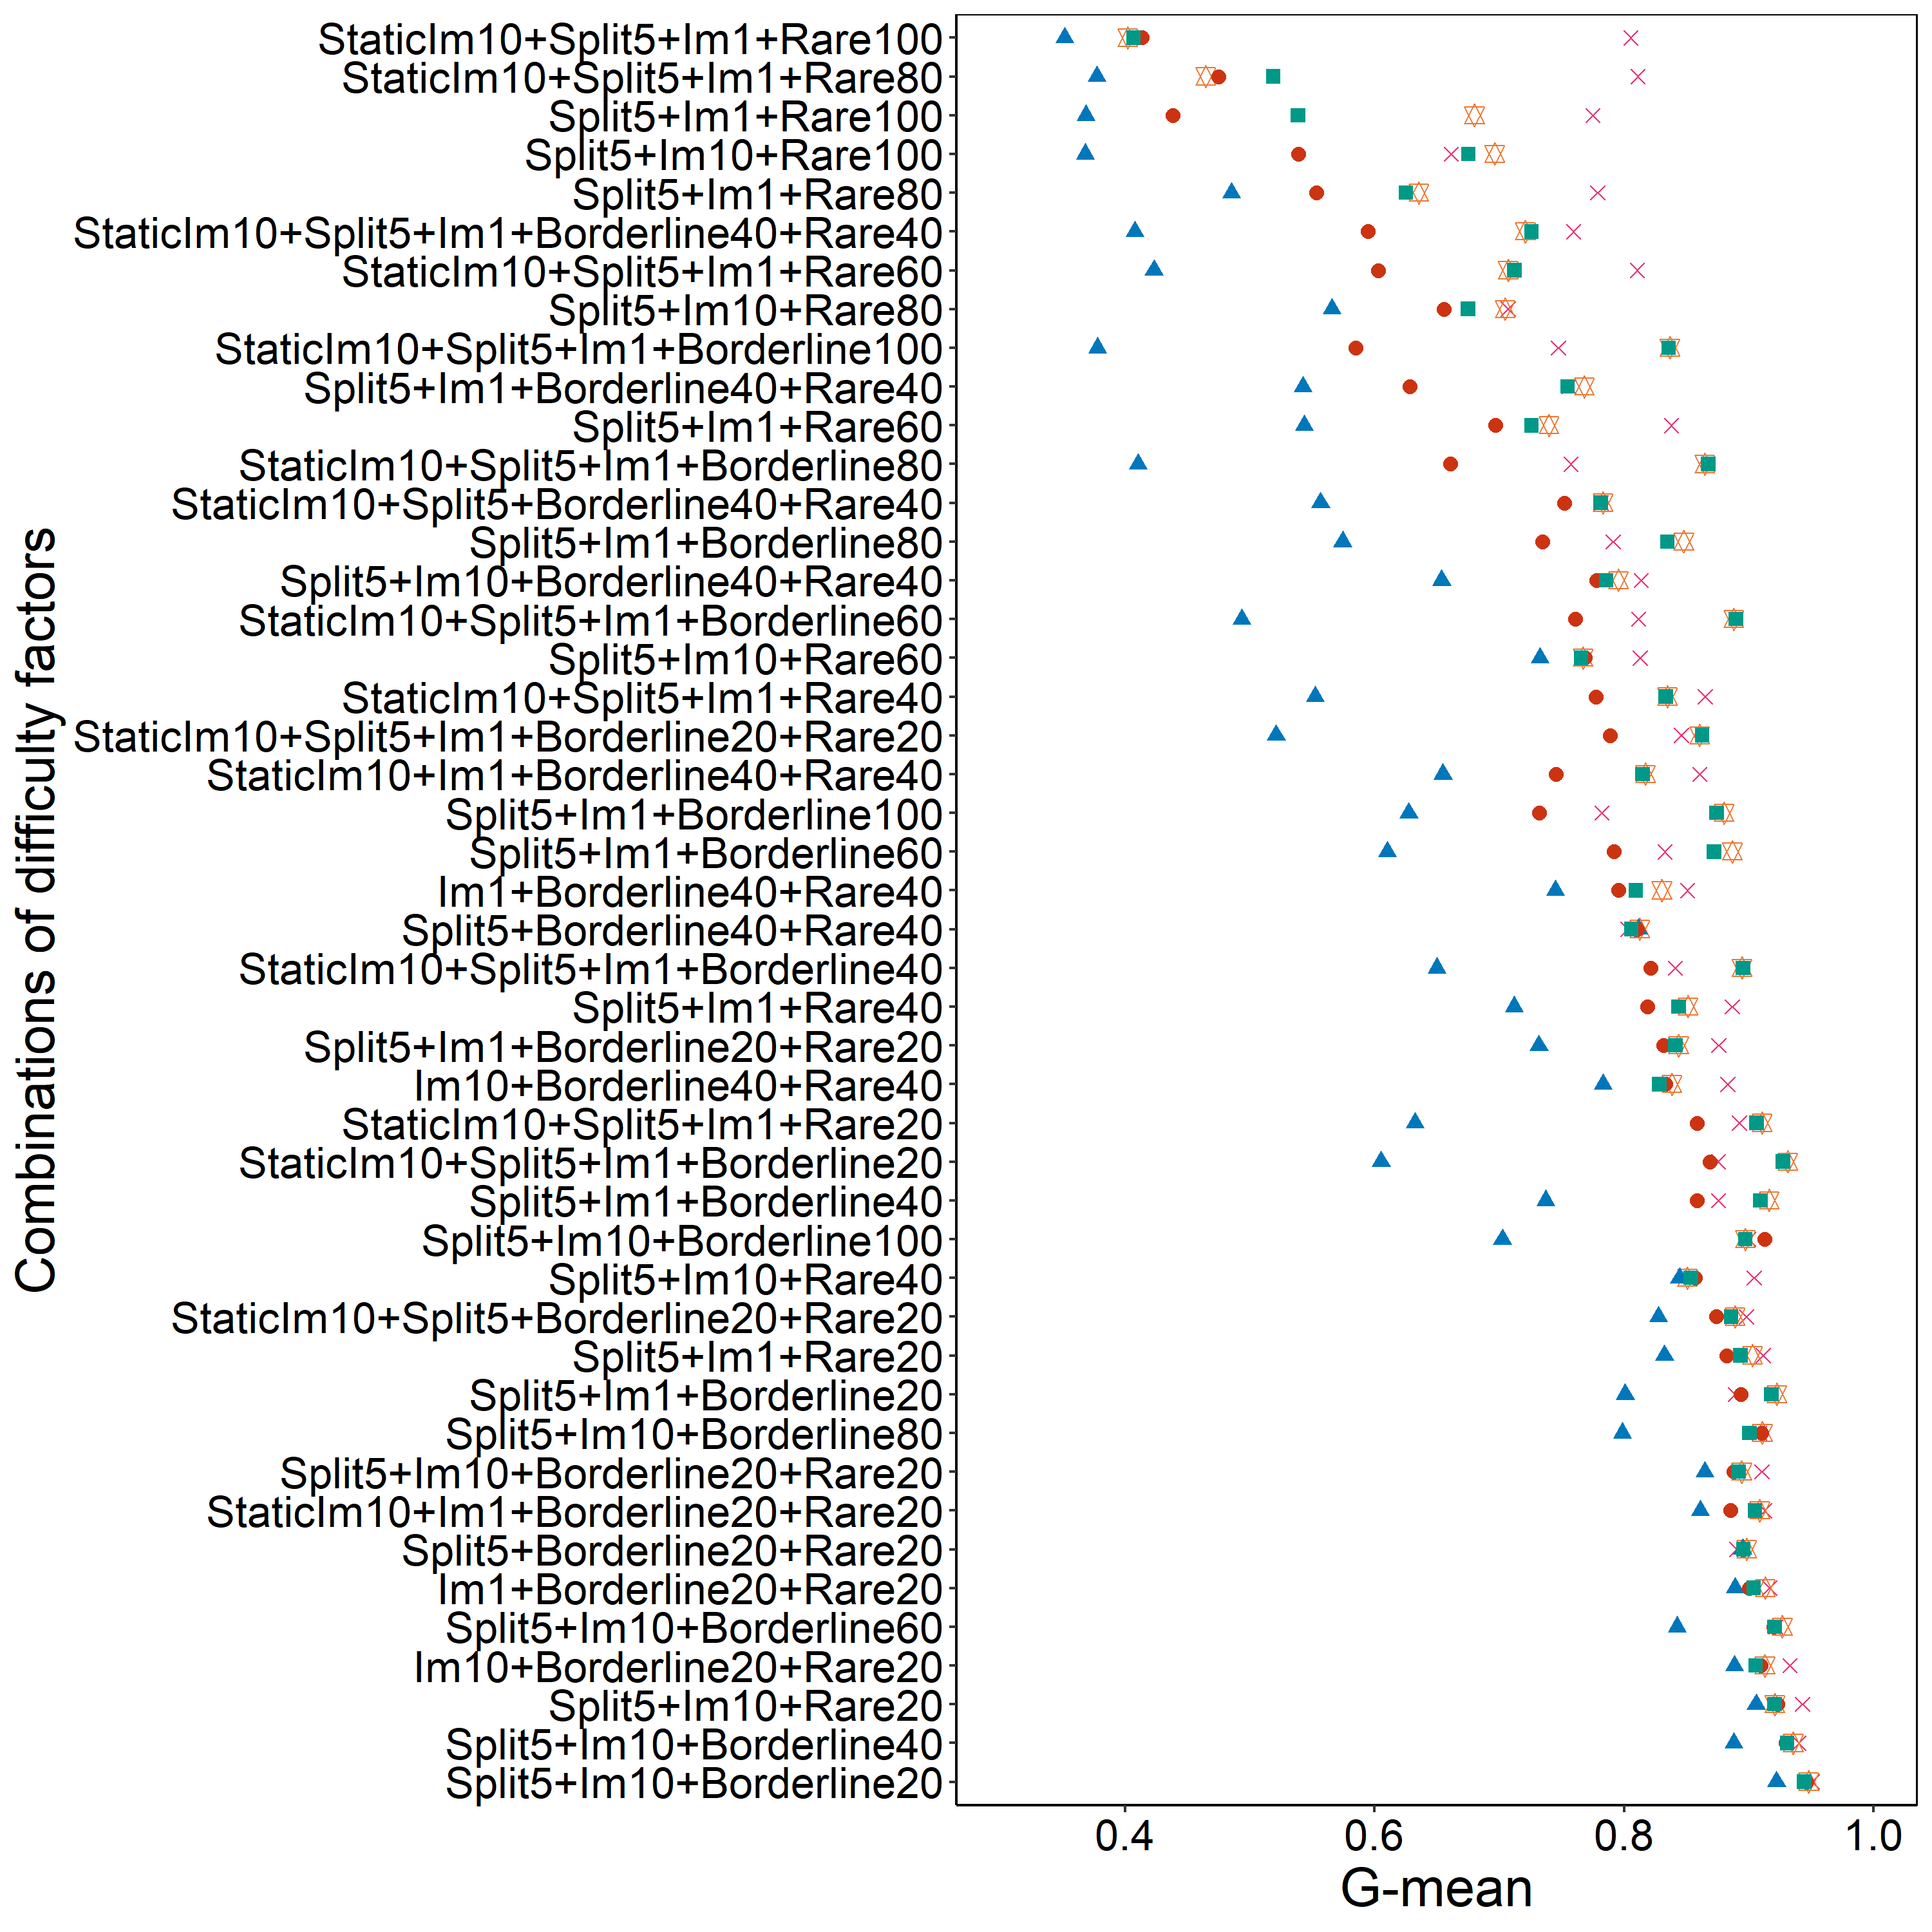
\includegraphics[width=7cm,height=9cm]{figures/complex_plot_G-mean.png}}
    \qquad
    \subfloat{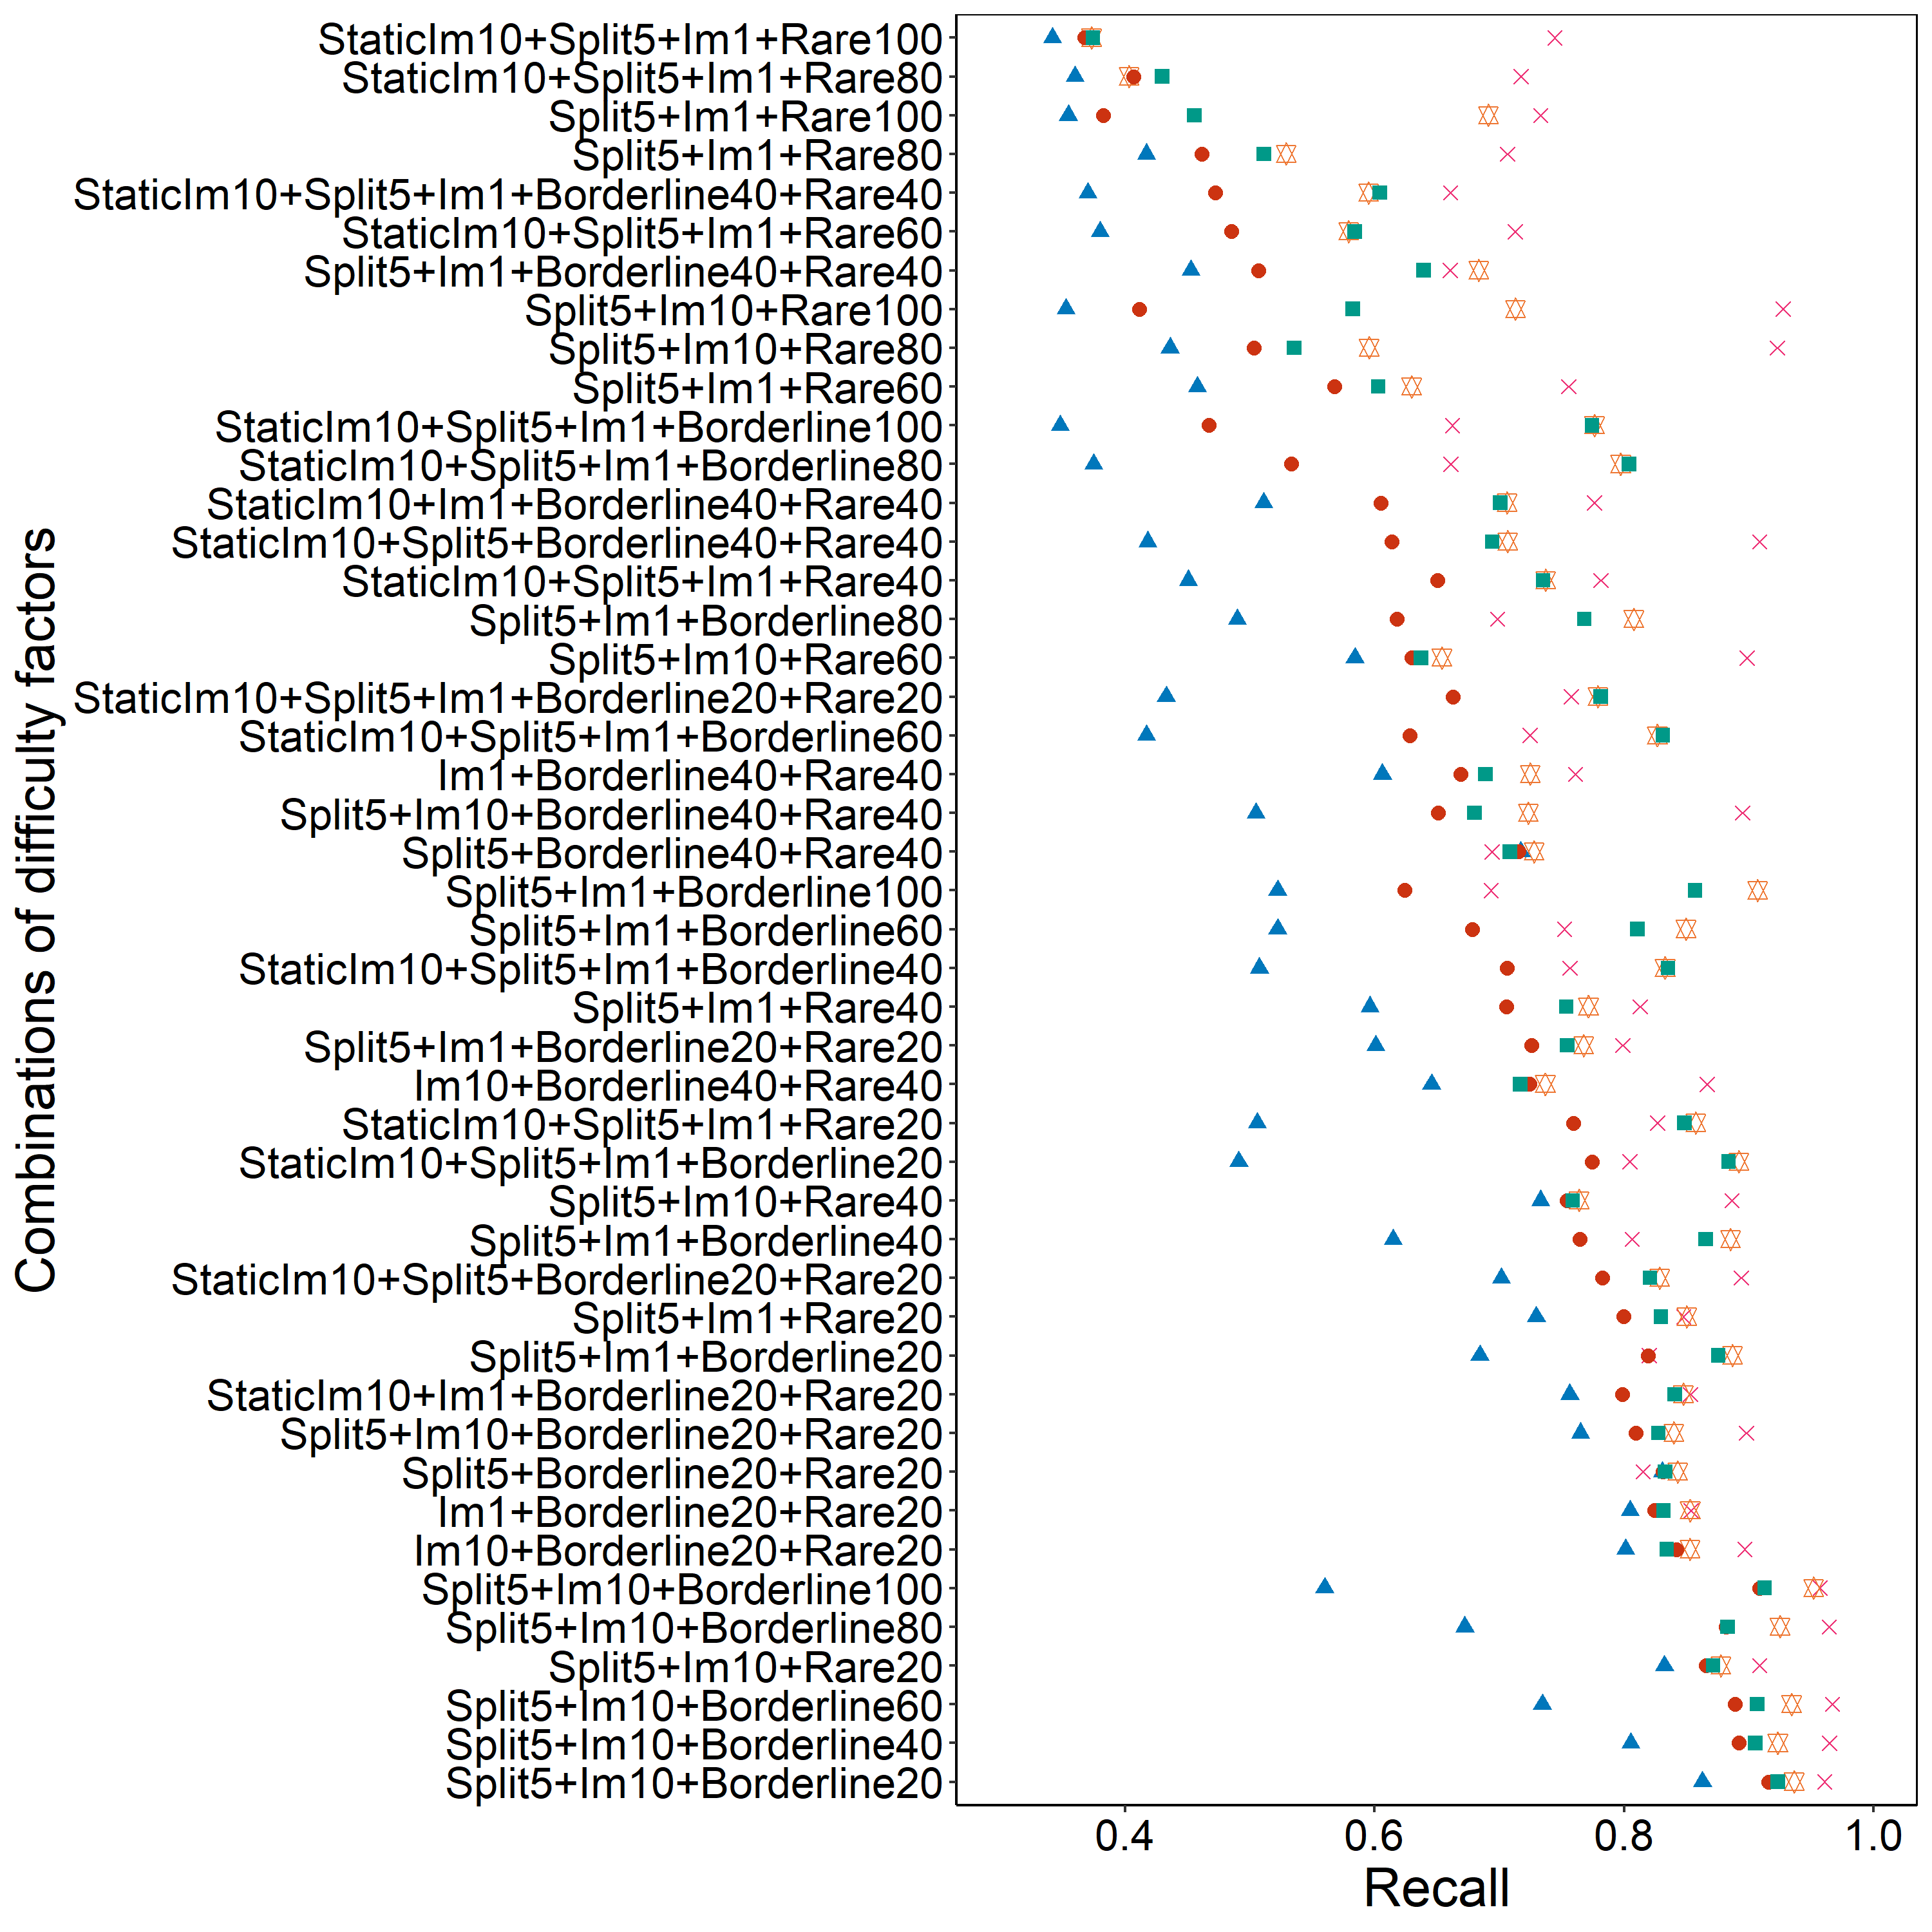
\includegraphics[width=7cm,height=9cm]{figures/complex_plot_Recall.png}}
    \caption{Porównanie jakości klasyfikacji na najbardziej wymagających strumieniach danych zawierających wiele czynników trudności}\label{Figure:ComplexComparison}
\end{figure}

\noindent Podobnie jak to było przy analizie strumieni z dwoma czynnikami trudności tak też tutaj można zauważyć, że algorytm \textit{NOOB} radzi sobie zdecydowanie lepiej od pozostałych algorytmów na najbardziej wymagających strumieniach danych. Obserwację tę potwierdzają wyniki otrzymane podczas analizy takich scenariuszy jak: \textit{StaticIm10+Split5+Im1+Rare100}, \textit{Split5+Im1Rare80}, \textit{StaticIm10+Split5+Im1+Rare60} - wyniki oscylującą w okolicy wartości 0.8 dla miary \textit{G-mean} oraz 0.7 dla miary \textit{Recall}. Należy także zwrócić uwagę, że drugi z zaproponowanych algorytmów \textit{NUOB} także daje sobie radę na analizowanych strumieniach. Wyróżniającymi się scenariuszami, pod kątem analizy obu miar, w tym przypadku były: \textit{Split5+Im10+Rare100}, \textit{Split5+Im1+Borderline40+Rare40}, \textit{Split5+Im1+Rare60}. Algorytmem, który charakteryzuje się najniższą jakością klasyfikacji, jest algorytm \textit{OB}, co potwierdza teorię, że poprzez losowanie z rozkładu Possiona z parametrem $\lambda$ = 1, algorytm ten nie będzie sobie w stanie odpowiednio poradzić na złożonych strumieniach danych.

W ramach tej sekcji przeprowadzono również porównanie statystyczne klasyfikatorów, jednak ze względu na mnogość kombinacji, zaprezentowane zostaną wyniki zbiorcze:

\begin{itemize}
    \item Na strumieniach danych zawierających co najmniej dwa czynniki trudności - \textit{multiple}
    \item Na wszystkich strumieniach danych - \textit{all}
\end{itemize}

\begin{table}[ht]
\centering\small%
\setlength{\tabcolsep}{10pt} 
\renewcommand{\arraystretch}{1.5} 
\begin{tabular}{l l c c c c c c}
\toprule
Data stream set & Metric & OB & UOB & OOB & NUOB & NOOB & CD \\
\midrule
Multiple & G-mean & 4.60 & 2.69 & 3.27 & \textbf{2.30} & \textbf{2.14} & 0.43 \\
All  & & 4.39 & \textbf{2.56} & 2.99 & \textbf{2.58} & \textbf{2.48} & 0.31 \\
Multiple & Recall & 4.67 & 2.61 & 3.76 & \textbf{1.79} & \textbf{2.17} & 0.43\\
All  & & 4.58 & 2.60 & 3.62 & \textbf{1.53} & 2.67 & 0.31 \\
\bottomrule
\end{tabular}
\caption{Wyniki przeprowadzonych testów statystycznych}\label{Tab:ComplexFriedman}
\end{table}

\noindent W tabeli \ref{Tab:ComplexFriedman} zestawione zostały wyniki przeprowadzonych testów statystycznych. Pod kątem kryterium przetwarzania na strumieniach danych zawierających co najmniej dwa czynniki trudności można wyszczególnić algorytmy: \textit{NUOB} oraz \textit{NOOB}. Biorąc pod uwagę wszystkie strumienie danych najlepiej prezentowały się algorytmy: \textit{UOB}, \textit{NUOB} oraz \textit{NOOB}.

\subsection{Podsumowanie}

\noindent W ramach niniejszego podrozdziału dokonano porównania algorytmów \textit{OB}, \textit{UOB}, \textit{OOB} z nowymi propozycjami algorytmów przetwarzania strumieniowego \textit{NUOB} oraz \textit{NOOB}. Przeprowadzona analiza została dokonana z podziałem na strumienie z jednym czynnikiem trudności (\english{single factors}), z dwoma czynnikami trudności (\english{pairs of factors}) oraz wieloma czynnikami trudności (\english{complex scenarios}).

Przeprowadzone testy na strumieniach z jednym czynnikiem trudności wykazały podobieństwo zaproponowanych algorytmów do już istniejących podejść pod kątem osiąganych wyników. Na wielu kryteriach otrzymane wyniki nie były statystycznie różne od najlepszych wyników. Pod kątem miary \textit{Recall} algorytm \textit{NUOB} okazał się najlepszy spośród wszystkich testowanych podejść.

Sytuacja lekko zmieniła się po przeprowadzeniu testów dla strumieni danych z dwoma i więcej czynnikami trudności. Nowo zaproponowane algorytmy \textit{NUOB} oraz \textit{NOOB} często osiągały najlepsze rezultaty na określonych scenariuszach. Przeprowadzone testy statystyczne także potwierdziły te obserwacje. Pod kątem miary \textit{G-mean} najlepszy okazał się algorytm \textit{NOOB}, a zaraz za nim kolejne miejsce zajął klasyfikator \textit{NUOB}. W przypadku miary \textit{Recall} sytuacja odwróciła się - najlepszy okazał się \textit{NUOB}, a zaraz za nim był \textit{NOOB}.

Wyniki przeprowadzonych testów pokazują, że zaproponowane w niniejszej pracy algorytmy charakteryzują się dobrymi wynikami w porównaniu do istniejących podejść, co może być potwierdzeniem realizacji założonego celu rozprawy.

\section{Hybrid Neighbourhood Online Bagging}

\noindent Przedstawiany w tej sekcji algorytm \textit{Hybrid Neighbourhood Online Bagging} składa się z dwóch klasyfikatorów składowych: \textit{Neighbourhood Undersampling Online Bagging} oraz \textit{Neighbourhood Oversampling Online Bagging}. Parametry używane w wymienionych algorytmach mają takie same wartości jak przy porównaniu, które zostało wykonane w ramach sekcji \ref{Section:AlgorithmsComparison}. Sprawa ma się podobnie dla algorytmów \textit{Oversampling Online Bagging} oraz \textit{Undersampling Online Bagging}, które także wykorzystują te same wartości parametrów, co przedstawione w sekcji wcześniejszej.

\subsection{Data streams with single factors}

\noindent Przedstawiany algorytm \textit{Hybrid Neighbourhood Online Bagging (HNOB)} charakteryzuje się tym, że stara się dopasować do aktualnie najlepszego pod względem miary \textit{G-mean} klasyfikatora składowego. Oznacza to, że bardzo często ten algorytm osiąga bardzo podobne wyniki, co lepsza z wersji algorytmów \textit{NUOB}, \textit{NOOB}. Efekt ten można m.in. zobaczyć na rysunkach \ref{Figure:Split7} oraz \ref{Figure:BorderlineRareHNOB}, gdzie podczas dryfu algorytm \textit{HNOB} dopasowuje się do aktualnie najlepszego algorytmu \textit{NUOB} i osiąga praktycznie identyczne wyniki.

\begin{figure}[h]
    \centering
    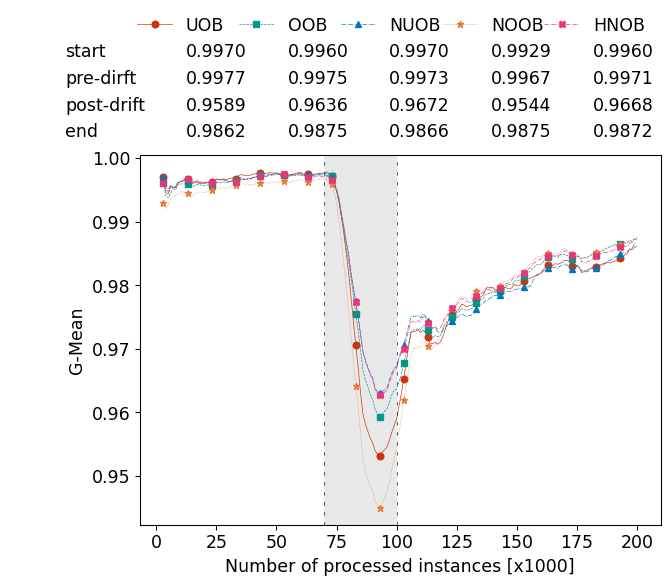
\includegraphics[width=11cm]{figures/split7_gmean.png}
    \caption{Wykres liniowy miary \textit{G-mean} dla strumienia \textit{Split7}}\label{Figure:Split7}
\end{figure}

\newpage

\begin{figure}[h]
    \centering
    \subfloat{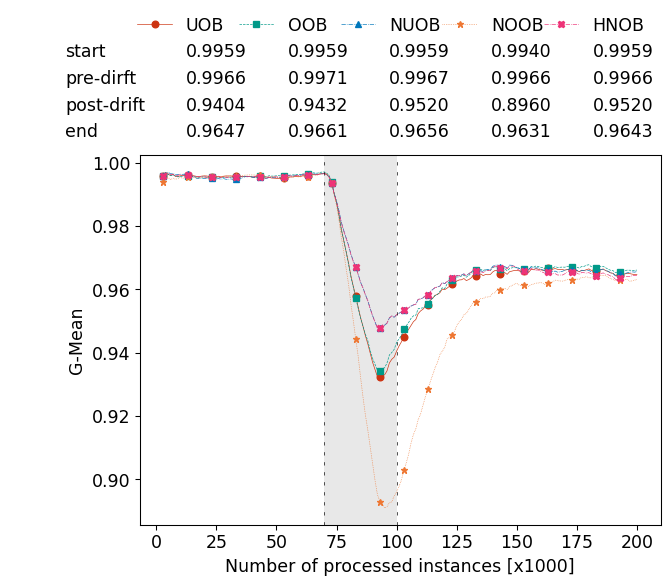
\includegraphics[width=7cm]{figures/borderline60_hnob_gmean.png}}
    \qquad
    \subfloat{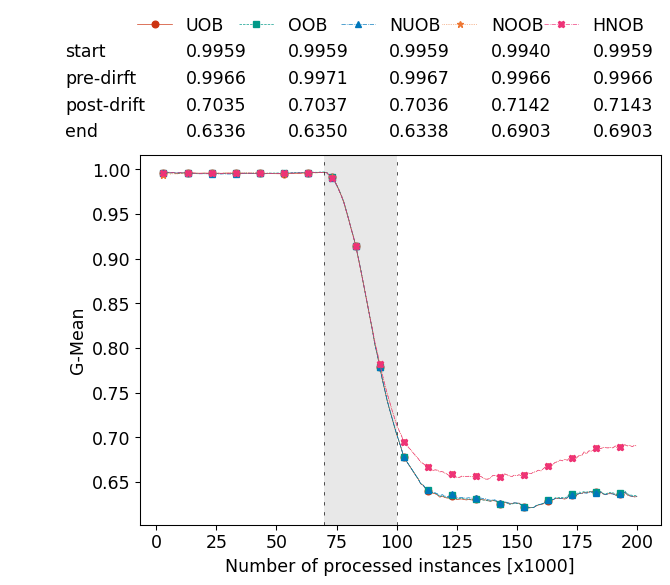
\includegraphics[width=7cm]{figures/rare60_hnob_gmean.png}}
    \caption{Wykresy liniowe miary \textit{G-mean} dla strumieni \textit{Borderline60} (po lewej) oraz \textit{Rare60} (po prawej)}\label{Figure:BorderlineRareHNOB}
\end{figure}

\noindent Aby ocenić jak radzi sobie algorytm \textit{HNOB} na strumieniach danych z jednym czynnikiem trudności, zdecydowano się przeprowadzić testy statystyczne z wykorzystaniem testu rang Friedman'a, którego kontynuacją będzie przeprowadzenie testu Nemenyi jako testu \textit{post hoc}. Wszystkie rezultaty zostały zweryfikowane na poziomie istotności $\alpha$ = 0.05.

\begin{table}[ht]
\centering\small%
\setlength{\tabcolsep}{10pt} 
\renewcommand{\arraystretch}{1.5} 
\begin{tabular}{l l c c c c c c}
\toprule
Data stream set & Metric & HNOB & UOB & OOB & NUOB & NOOB & CD \\
\midrule
Static imbalance & G-mean & \textbf{3.06} & \textbf{2.06} & \textbf{2.65} & \textbf{3.29} & 3.94 & 1.51 \\
Class ratio changes & & 2.70 & \textbf{1.84} & 3.25 & 3.47 & 3.73 & 0.77 \\
Sub-cluster merge & & \textbf{2.17} & \textbf{3.83} & \textbf{2.63} & \textbf{3.00} & \textbf{3.33} & 2.68 \\
Sub-cluster move & & \textbf{1.50} & 4.83 & \textbf{1.83} & \textbf{4.17} & \textbf{2.67} & 2.68 \\
Sub-cluster split & & \textbf{1.67} & 4.50 & \textbf{2.33} & \textbf{2.33} & \textbf{4.17} & 2.68 \\
Borderline examples & & \textbf{2.50} & \textbf{3.80} & \textbf{2.10} & \textbf{2.50} & \textbf{4.10} & 2.01 \\
Rare examples & & \textbf{2.30} & \textbf{3.90} & \textbf{2.50} & \textbf{4.00} & \textbf{2.30} & 2.01 \\
Static imbalance & Recall & 3.24 & 2.59 & 3.82 & \textbf{1.00} & 4.35 & 1.51 \\
Class ratio changes & & 2.64 & 2.63 & 4.48 & \textbf{1.02} & 4.23 & 0.77 \\
Sub-cluster merge & & \textbf{3.00} & \textbf{3.33} & \textbf{2.67} & \textbf{1.00} & 5.00 & 2.68 \\
Sub-cluster move & & 3.83 & \textbf{2.83} & \textbf{2.33} & \textbf{1.00} & 5.00 & 2.68 \\
Sub-cluster split & & \textbf{2.83} & \textbf{3.67} & \textbf{2.50} & \textbf{1.00} & 5.00 & 2.68 \\
Borderline examples & & \textbf{3.00} & 3.40 & \textbf{2.60} & \textbf{1.00} & 5.00 & 2.01 \\
Rare examples & & \textbf{2.20} & \textbf{4.00} & \textbf{3.40} & \textbf{2.50} & \textbf{2.90} & 2.01 \\
\bottomrule
\end{tabular}
\caption{Wyniki przeprowadzonych testów statystycznych dla pojedynczych czynników trudności}\label{Tab:SingleDriftFriedmanHNOB}
\end{table}

\noindent W tabeli \ref{Tab:SingleDriftFriedmanHNOB} przedstawione zostały wyniki przeprowadzonych testów statystycznych. Pogrubione zostały najlepsze wyniki dla określonych zbiorów danych oraz wyniki, które okazały się nie być statystycznie różne od najlepszego wyniku. Na podstawie otrzymanych rezultatów możliwe jest określenie rankingu algorytmów pod kątem danej miary:

\begin{itemize}
    \item \textit{G-mean} - HNOB, OOB, NUOB $\succ$ UOB, NOOB
    \item \textit{Recall} - NUOB $\succ$ OOB $\succ$ HNOB, UOB $\succ$ NOOB
\end{itemize}

\subsection{Data streams with pairs of factors}

\noindent W przypadku analizy strumieni danych z dwoma czynnikami trudności można się spodziewać, że algorytm hybrydowy poradzi sobie lepiej aniżeli przy analizie strumieni danych z jednym czynnikiem trudności. Jest to spowodowane faktem, że wcześniejsza analiza wykazała, że najlepszymi algorytmami były \textit{NOOB} oraz \textit{NUOB}. Algorytm hybrydowy powinien zaaplikować zalety obu tych klasyfikatorów w swoim działaniu. Aby zweryfikować tę tezę, zestawiono wyniki wszystkich algorytmów na najbardziej wymagających strumieniach danych. Otrzymane wyniki widoczne są na rysunku \ref{Figure:PairsComparisonHNOB}.

\begin{figure}[h]
    \centering
    \subfloat{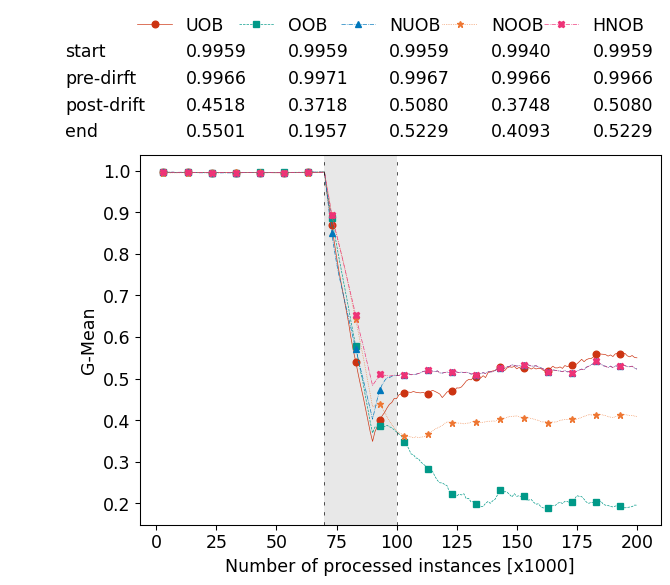
\includegraphics[width=7cm]{figures/im10rare100_hnob_gmean.png}}
    \qquad
    \subfloat{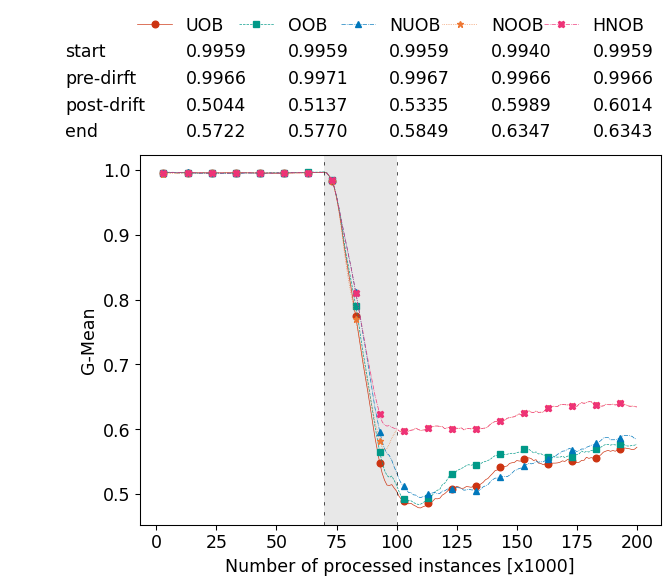
\includegraphics[width=7cm]{figures/split5rare80_hnob_gmean.png}}
    \caption{Wykresy liniowe miary \textit{G-mean} dla strumieni \textit{Im10+Rare100} (po lewej) oraz \textit{Split5+Rare80} (po prawej)}\label{Figure:PairsFactorsHNOB}
\end{figure}

\begin{figure}[h]
    \centering
    \subfloat{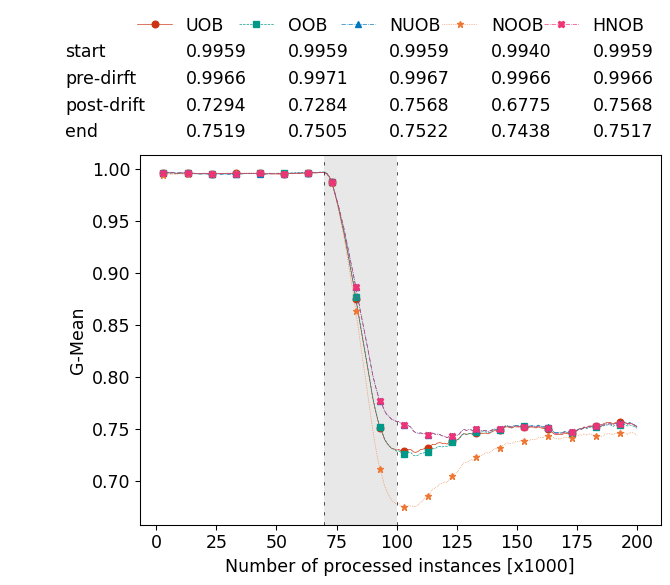
\includegraphics[width=7cm]{figures/borderline40rare80_hnob_gmean.png}}
    \qquad
    \subfloat{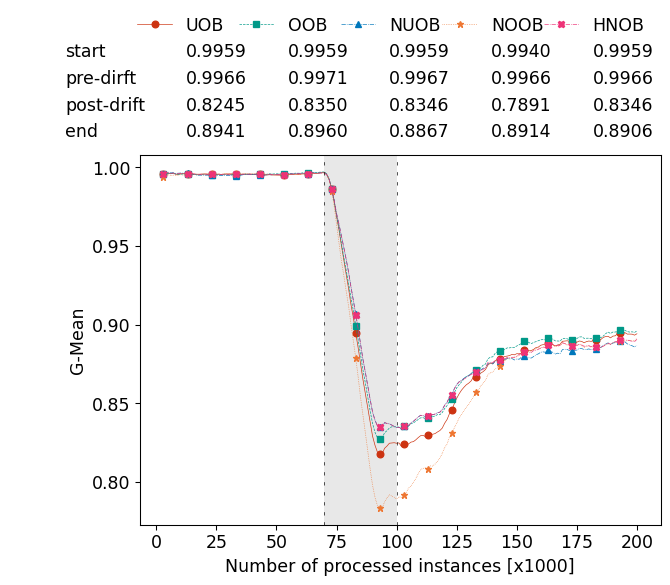
\includegraphics[width=7cm]{figures/split5borderline80_hnob_gmean.png}}
    \caption{Wykresy liniowe miary \textit{G-mean} dla strumieni \textit{Borderline40+Rare40} (po lewej) oraz \textit{Split5+Borderline80} (po prawej)}
\end{figure}

\newpage

\begin{figure}[h]
    \centering
    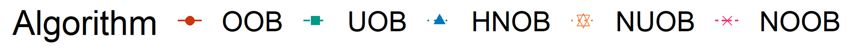
\includegraphics[width=7cm]{figures/algorithms_legend_hnob.JPG}
\end{figure}

\vspace{-1.2cm}

\begin{figure}[h]
    \centering
    \subfloat{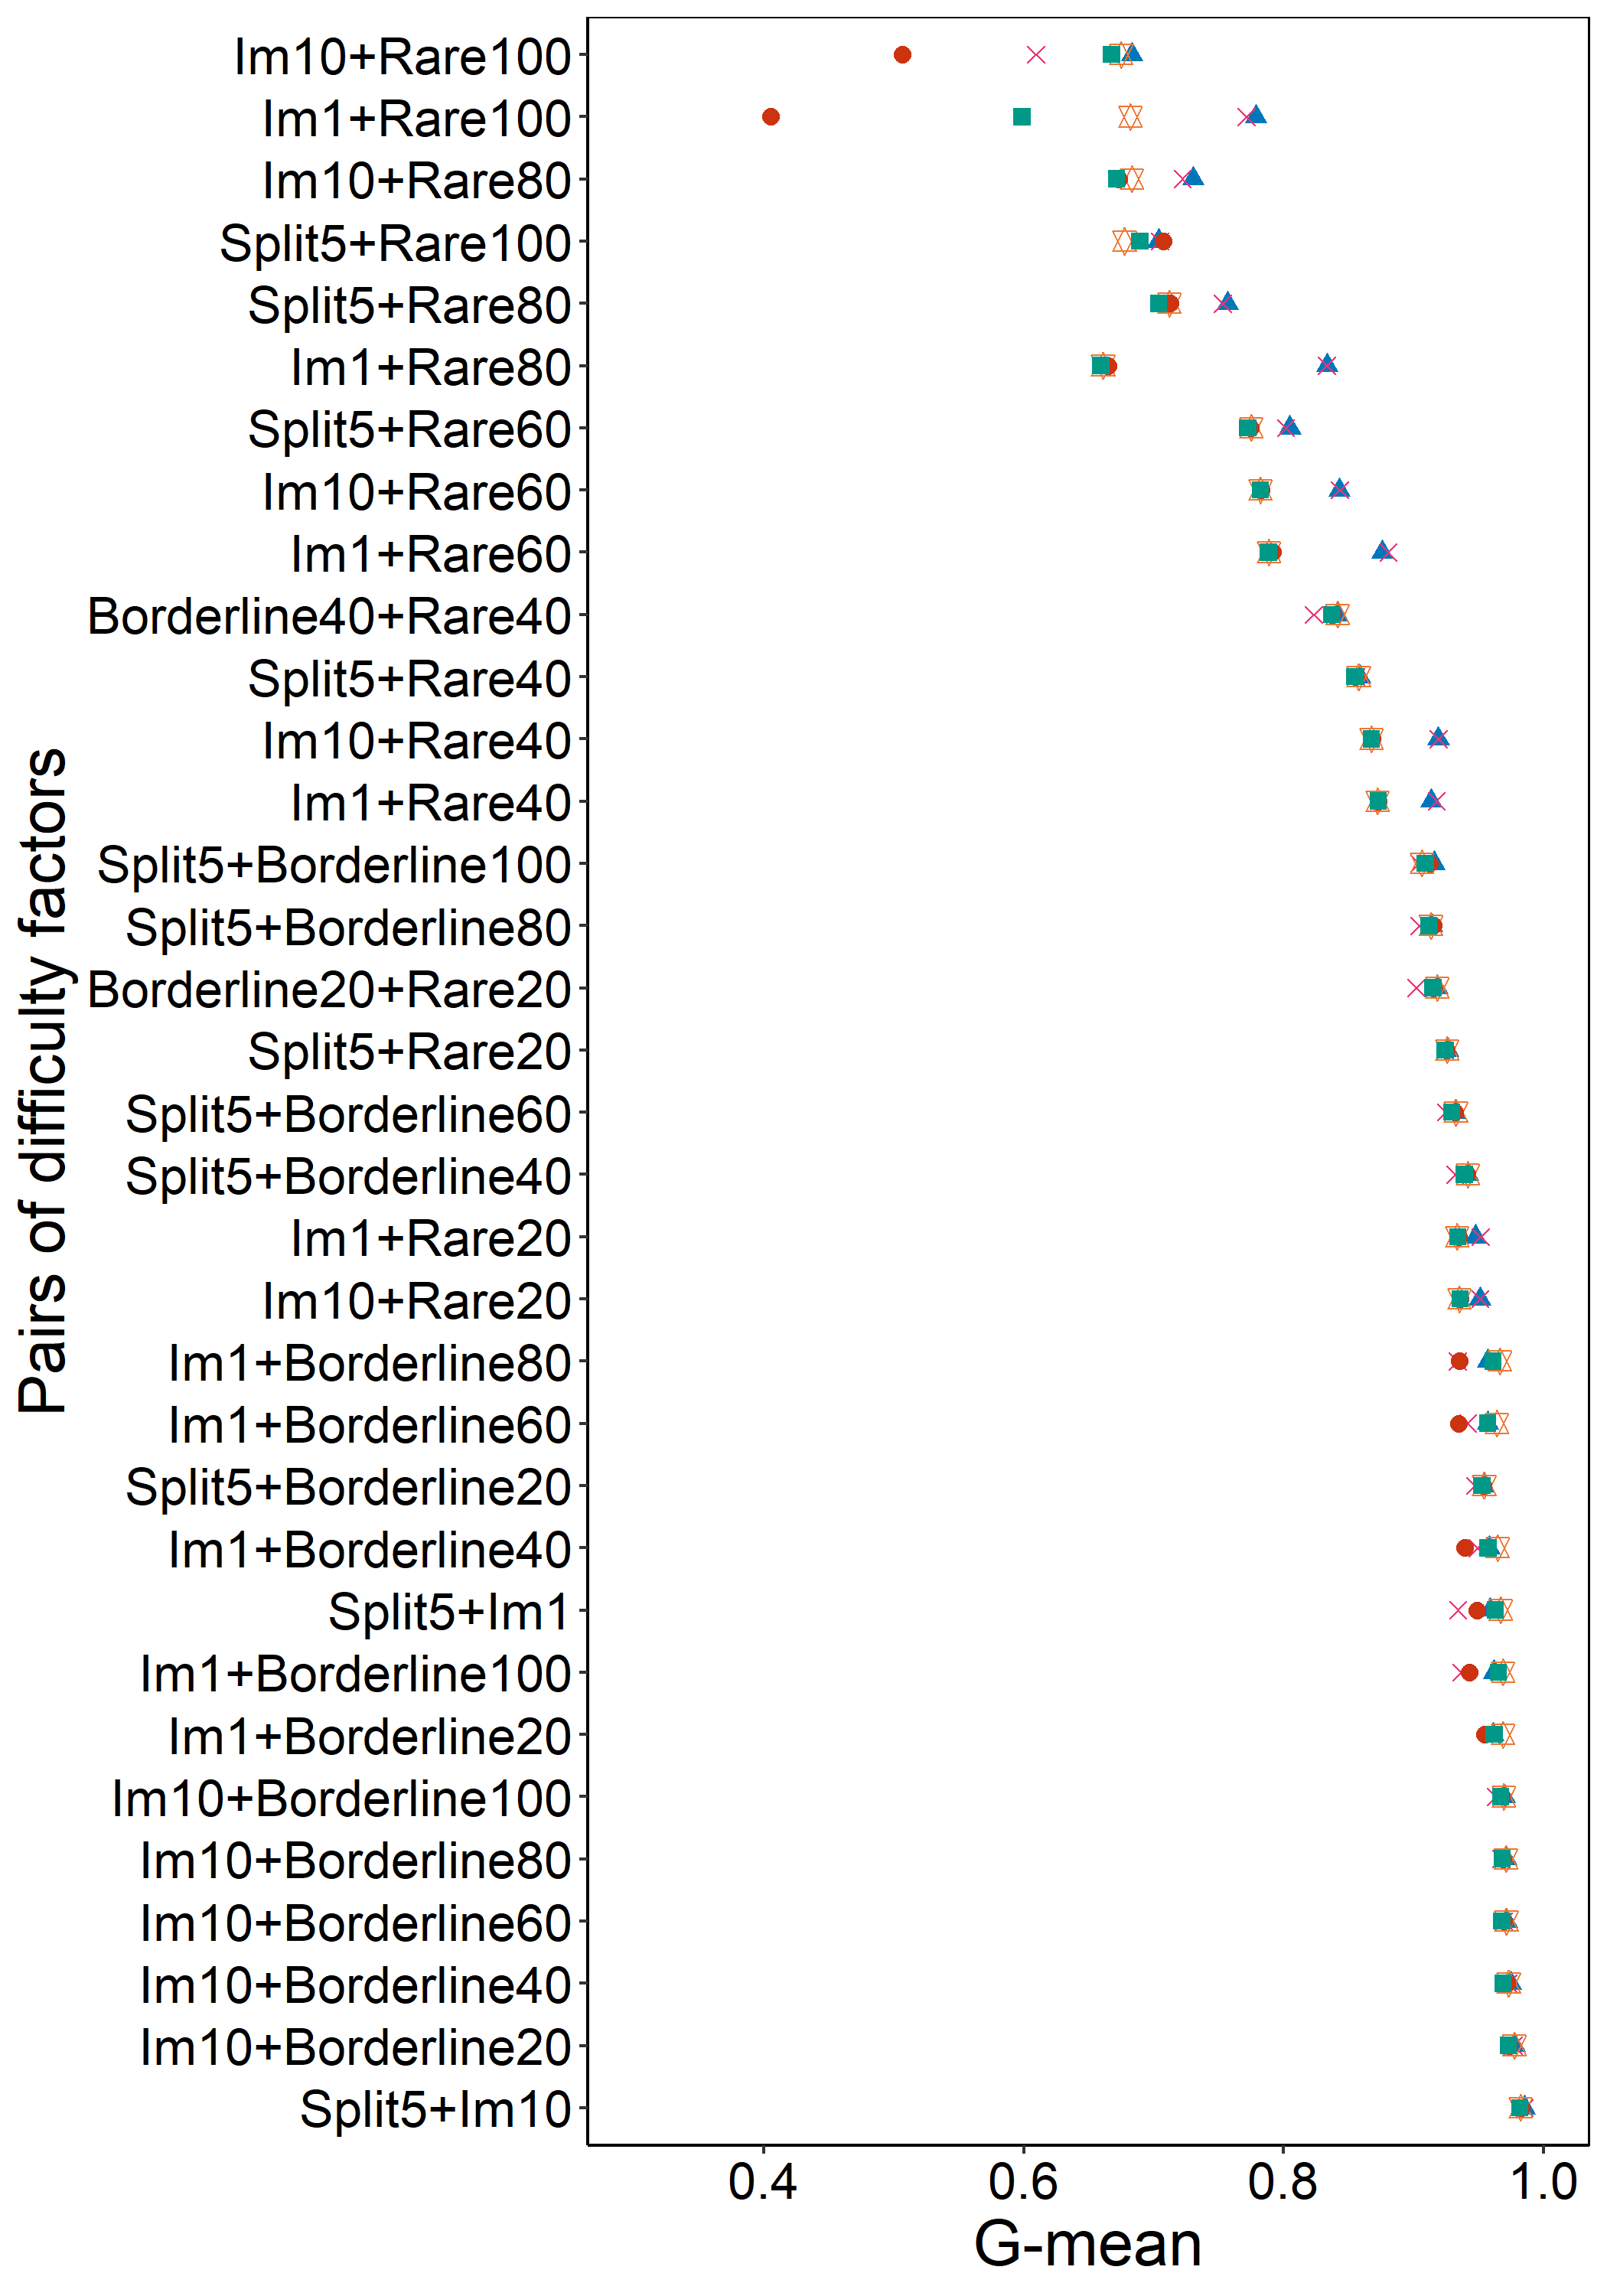
\includegraphics[width=7cm]{figures/pair_plot_G-mean_HNOB.png}}
    \qquad
    \subfloat{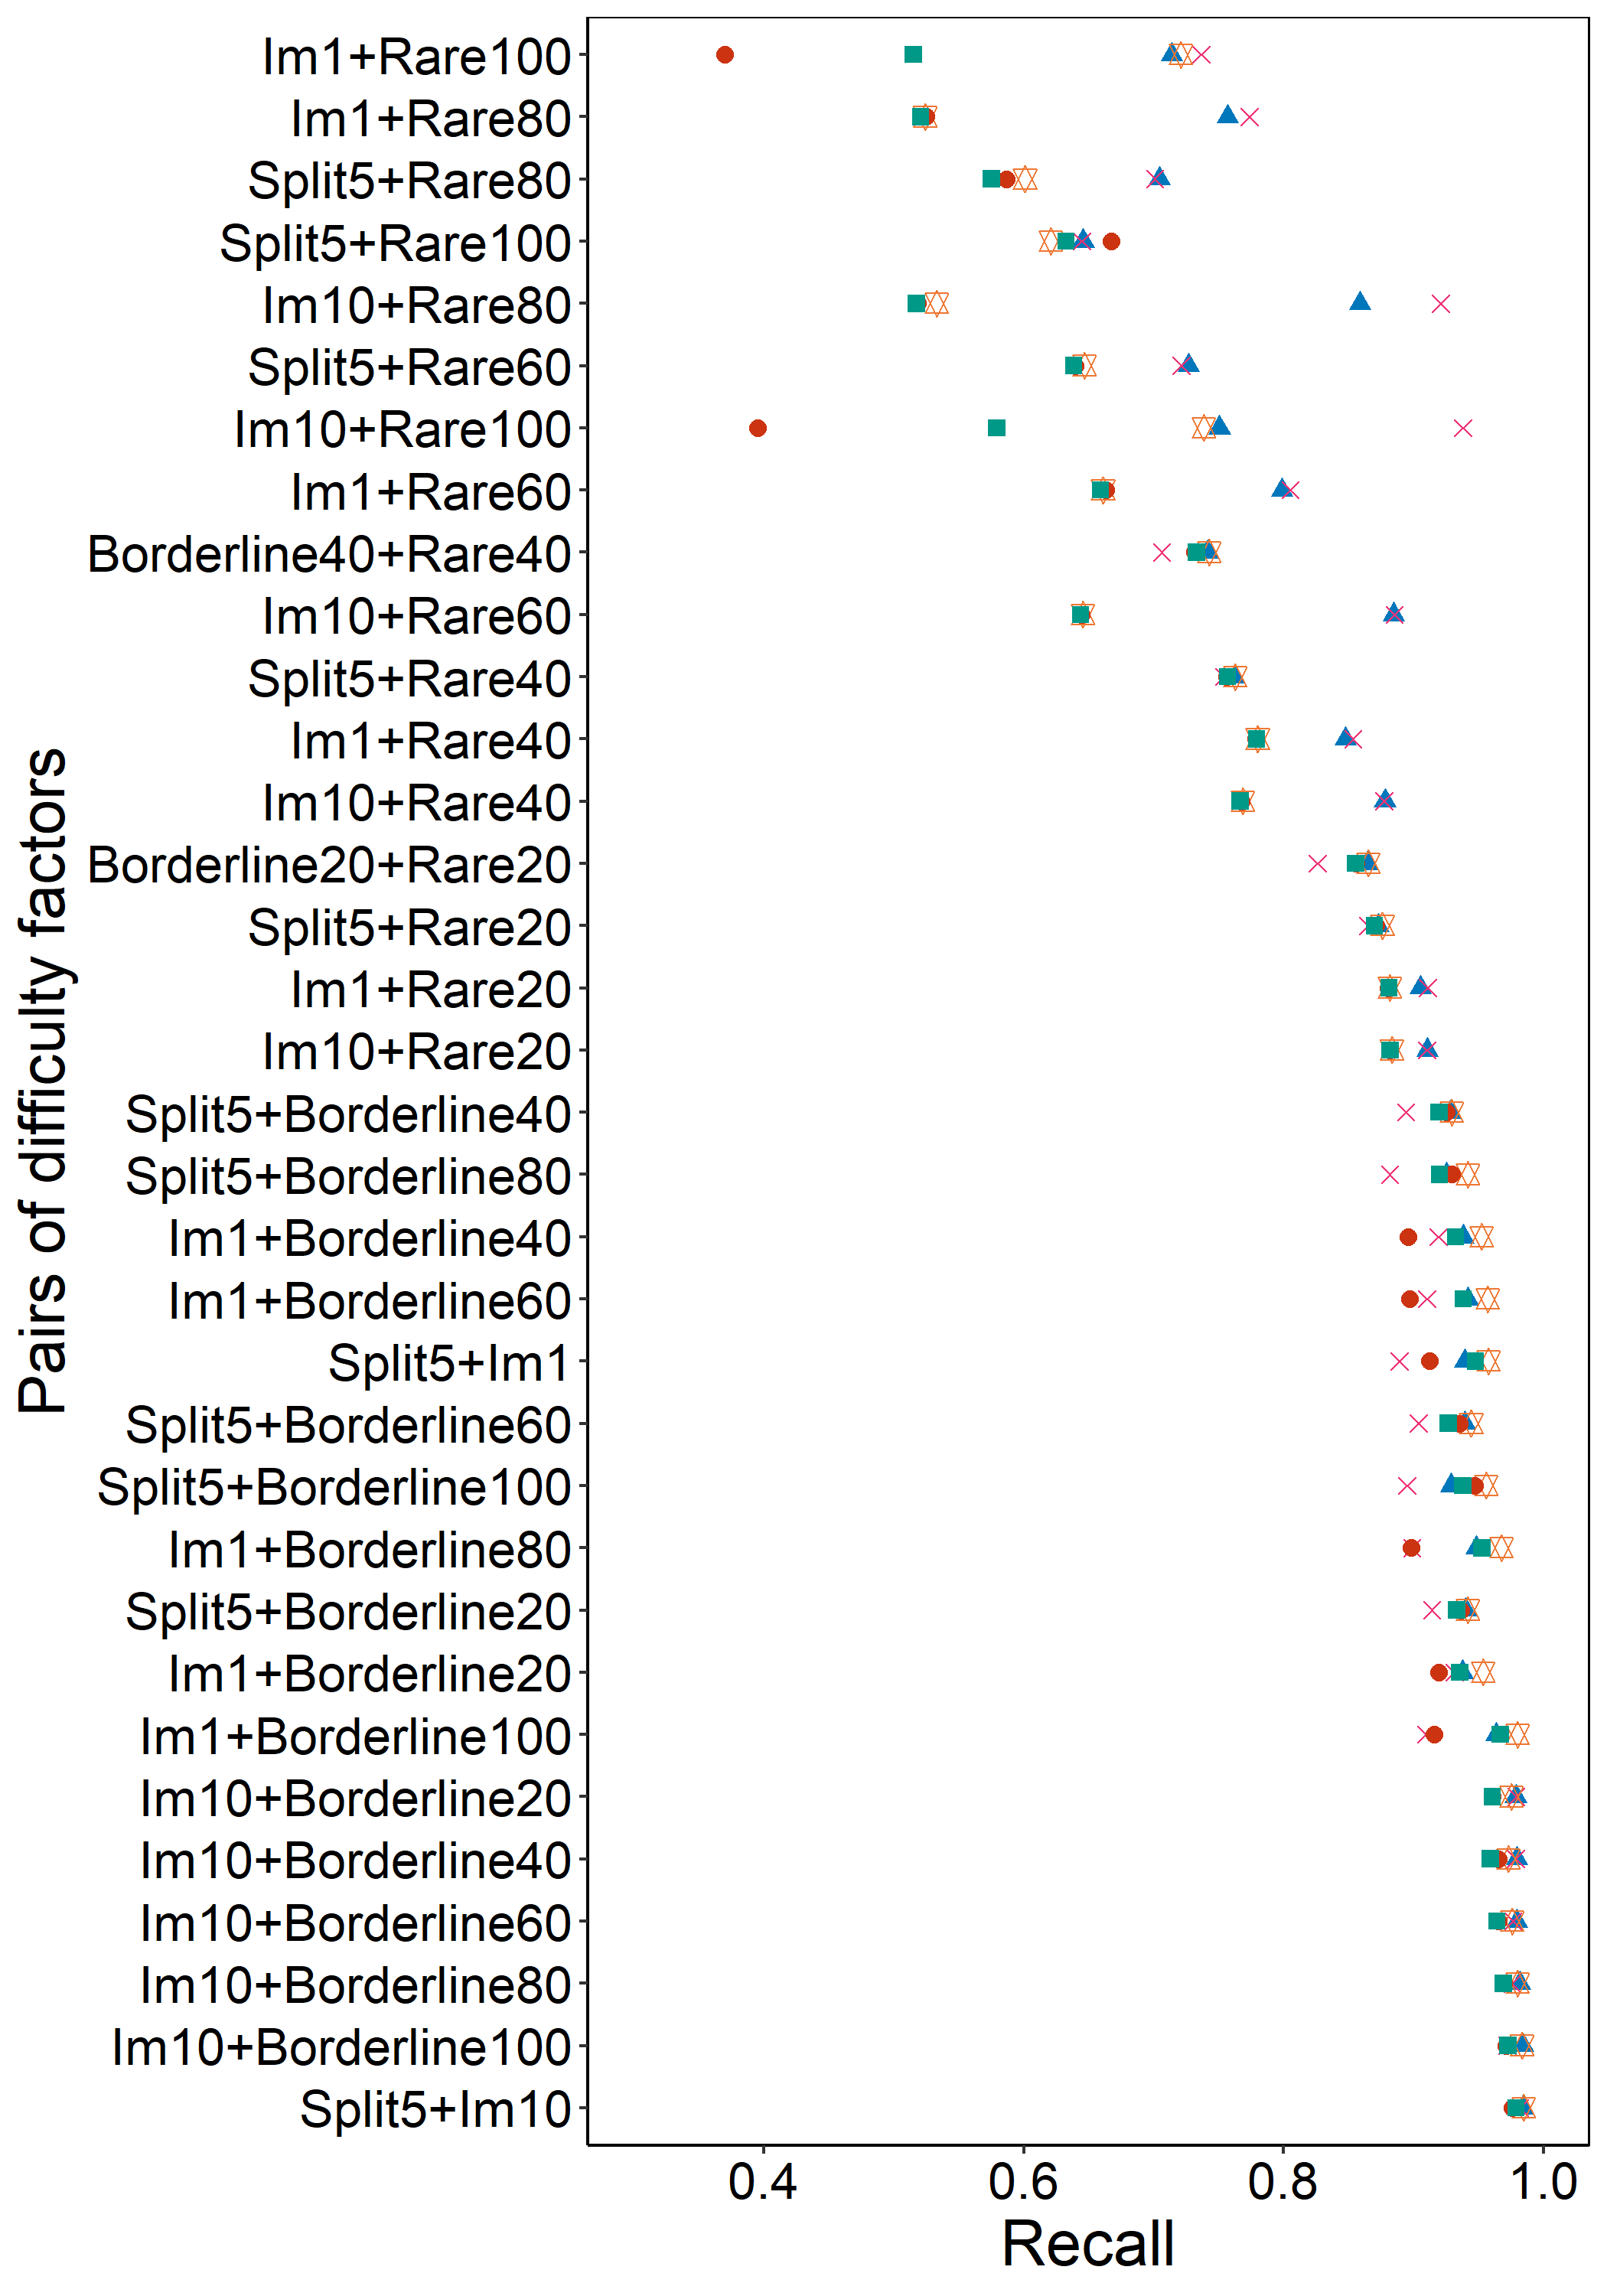
\includegraphics[width=7cm]{figures/pair_plot_Recall_HNOB.png}}
    \caption{Porównanie jakości klasyfikacji na najbardziej wymagających strumieniach danych zawierających dwa czynniki trudności}\label{Figure:PairsComparisonHNOB}
\end{figure}

\noindent Jak można zauważyć na ilustracji \ref{Figure:PairsComparisonHNOB} wysunięta teza okazała się prawdziwa w przypadku scenariuszy analizowanych pod kątem miary \textit{G-mean}. Algorytm hybrydowy osiąga rezultaty bardzo zbliżone do aktualnie najlepszego algorytmu. Można to zaobserwować w przypadku analizy takich scenariuszy, jak np. \textit{Im10+Rare40}, \textit{Im10+Rare60}, \textit{Split5+Rare60}. Sytuacja zmienia się trochę dla niektórych przykładów strumieni pod kątem miary \textit{Recall}. Dla większości przypadków można zauważyć, że algorytm \textit{HNOB} osiąga bardzo podobne wyniki, co najlepszy z algorytmów. Istnieją jednak takie instancje jak np. \textit{Im10+Rare80} lub \textit{Im10+Rare100}, gdzie klasyfikator \textit{HNOB} odbiega swoim wynikiem od aktualnie najlepszego klasyfikatora. Spowodowane to jest faktem, że podejście hybrydowe dopasowuje się z wykorzystaniem miary \textit{G-mean}, wobec czego dopasowanie musiało nastąpić do algorytmu \textit{NUOB}, który charakteryzował się wyższą wartością miary \textit{G-mean} aniżeli algorytm \textit{NOOB}.

Analiza statystyczna algorytmów dla strumieni danych zawierających dwa czynniki trudności została przedstawiona w tabeli \ref{Tab:DoubleDriftFriedmanHNOB}.

\newpage

\begin{table}[ht]
\centering\small%
\setlength{\tabcolsep}{10pt} 
\renewcommand{\arraystretch}{1.5} 
\begin{tabular}{l l c c c c c c}
\toprule
Data stream set & Metric & HNOB & UOB & OOB & NUOB & NOOB & CD \\
\midrule
Imbalance + Move & G-mean & \textbf{2.17} & \textbf{2.83} & \textbf{3.75} & \textbf{3.17} & \textbf{3.08} & 1.82 \\
Imbalance + Merge  & & \textbf{2.08} & \textbf{2.17} & 4.08 & \textbf{2.75} & 3.92 & 1.82 \\
Imbalance + Split  & & \textbf{2.17} & \textbf{2.67} & 4.50 & \textbf{2.44} & \textbf{3.22} & 1.47 \\
Imbalance + Borderline  & & \textbf{2.17} & \textbf{2.92} & 4.38 & \textbf{2.08} & 3.45 & 0.97 \\
Imbalance + Rare  & & \textbf{1.63} & 3.77 & 4.08 & 3.88 & \textbf{1.65} & 0.97 \\
Split + Borderline  & & \textbf{2.10} & \textbf{2.90} & 4.00 & \textbf{2.38} & 3.62 & 0.87 \\
Split + Rare  & & \textbf{1.56} & 3.64 & 4.14 & 3.56 & \textbf{2.10} & 0.87 \\
Imbalance + Move & Recall & \textbf{2.50} & \textbf{2.50} & 4.83 & \textbf{1.58} & 3.58 & 1.82 \\
Imbalance + Merge  & & \textbf{2.42} & \textbf{2.32} & 4.83 & \textbf{1.67} & 3.75 & 1.82 \\
Imbalance + Split  & & \textbf{2.39} & \textbf{2.56} & 4.83 & \textbf{1.56} & 3.67 & 1.47 \\
Imbalance + Borderline  & & \textbf{2.20} & 3.10 & 4.88 & \textbf{1.75} & 3.08 & 0.97 \\
Imbalance + Rare  & & \textbf{1.95} & 3.58 & 4.83 & 2.90 & \textbf{1.75} & 0.97 \\
Split + Borderline  & & \textbf{2.46} & 3.00 & 4.48 & \textbf{2.04} & 3.02 & 0.87 \\
Split + Rare  & & \textbf{2.14} & 3.28 & 4.56 & \textbf{2.76} & \textbf{2.26} & 0.87 \\
\bottomrule
\end{tabular}
\caption{Wyniki przeprowadzonych testów statystycznych dla par czynników trudności}\label{Tab:DoubleDriftFriedmanHNOB}
\end{table}

\noindent W tabeli \ref{Tab:DoubleDriftFriedmanHNOB} zestawione zostały wyniki przeprowadzonych testów statystycznych. Pogrubione zostały najlepsze wyniki dla określonych zbiorów danych oraz wyniki, które okazały się nie być statystycznie różne od najlepszego wyniku. Na podstawie otrzymanych rezultatów możliwe jest określenie rankingu algorytmów pod kątem danej miary:

\begin{itemize}
    \item \textit{G-mean} - HNOB $\succ$ UOB, NUOB $\succ$ NOOB $\succ$ OOB
    \item \textit{Recall} - HNOB $\succ$ NUOB $\succ$ UOB $\succ$ NOOB $\succ$ OOB
\end{itemize}

\subsection{Complex scenarios}

\noindent Analiza algorytmów pod kątem strumieni danych z wieloma czynnikami trudności będzie przebiegać w podobny sposób jak dla strumieni z dwoma czynnikami trudności. W pierwszej kolejności wyniki wszystkich podejść zostaną zaprezentowane na wykresie zawierającym najbardziej wymagające strumienie danych pod kątem jakości klasyfikacji. W drugiej części zostanie przedstawione zestawienie statystyczne na sekwencjach danych zawierających co najmniej dwa czynniki trudności oraz na wszystkich sekwencjach danych.

\newpage

\begin{figure}[h]
    \centering
    \subfloat{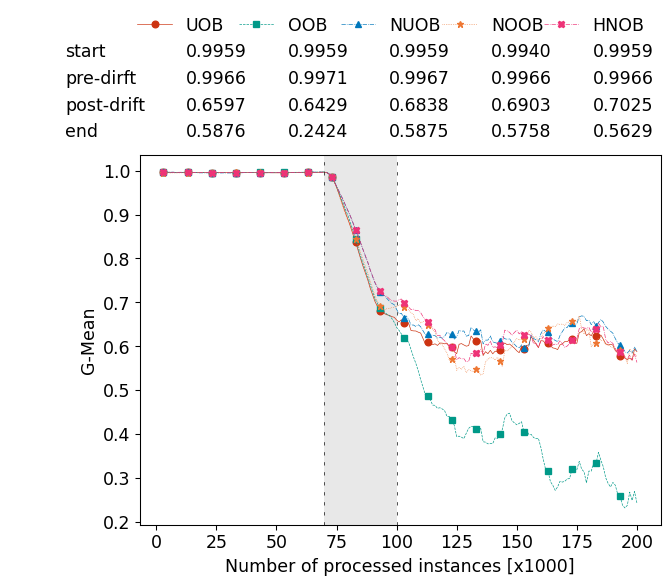
\includegraphics[width=7cm]{figures/split5im1borderline40rare40_hnob_gmean.png}}
    \qquad
    \subfloat{\includegraphics[width=7cm]{figures/staticim10im1rare80_hnob_gmean.png}}
    \caption{Wykresy liniowe miary \textit{G-mean} dla strumieni \textit{Split5+Im1+Borderline40+Rare40} (po lewej) oraz \textit{StaticIm10+Im1+Rare80} (po prawej)}
\end{figure}

\begin{figure}[h]
    \centering
    \includegraphics[width=7cm]{figures/algorithms_legend_hnob.JPG}
\end{figure}

\vspace{-1.2cm}

\begin{figure}[h]
    \centering
    \subfloat{\includegraphics[width=7cm,height=9cm]{figures/complex_plot_G-mean_HNOB.png}}
    \qquad
    \subfloat{\includegraphics[width=7cm,height=9cm]{figures/complex_plot_Recall_HNOB.png}}
    \caption{Porównanie jakości klasyfikacji na najbardziej wymagających strumieniach danych zawierających wiele czynników trudności}\label{Figure:ComplexComparisonHNOB}
\end{figure}

\newpage

\begin{table}[ht]
\centering\small%
\setlength{\tabcolsep}{10pt} 
\renewcommand{\arraystretch}{1.5} 
\begin{tabular}{l l c c c c c c}
\toprule
Data stream set & Metric & HNOB & UOB & OOB & NUOB & NOOB & CD \\
\midrule
Multiple & G-mean & \textbf{1.87} & 3.31 & 4.16 & 2.86 & 2.80 & 0.43 \\
All  & & \textbf{2.09} & 3.02 & 3.76 & 3.03 & 3.10 & 0.31 \\
Multiple & Recall & \textbf{2.25} & 3.15 & 4.63 & \textbf{2.32} & \textbf{2.66} & 0.43\\
All  & & 2.41 & 3.04 & 4.42 & \textbf{1.89} & 3.23 & 0.31 \\
\bottomrule
\end{tabular}
\caption{Wyniki przeprowadzonych testów statystycznych}\label{Tab:ComplexFriedmanHNOB}
\end{table}

\noindent Na rysunku \ref{Figure:ComplexComparisonHNOB} można zaobserwować wyniki analizowanych algorytmów na najbardziej wymagających strumieniach danych zawierających wiele czynników trudności. Obserwując wyniki algorytmu \textit{HNOB} można wyciągnąć bardzo podobne wnioski jak przy analizie strumieni z dwoma czynnikami trudności. Bardzo widoczne jest dopasowanie do aktualnie najlepszego algorytmu analizując miarę \textit{G-mean}.

W tabeli \ref{Tab:ComplexFriedmanHNOB} zestawione zostały wyniki przeprowadzonych testów statystycznych. Pod kątem kryterium przetwarzania na strumieniach danych zawierających co najmniej dwa czynniki trudności można wyszczególnić algorytm \textit{HNOB}. Biorąc pod uwagę wszystkie strumienie danych najlepiej prezentowały się algorytmy: \textit{HNOB}, \textit{NUOB} oraz \textit{NOOB}.

\subsection{Podsumowanie}

\noindent W ramach niniejszego podrozdziału dokonano porównania algorytmów \textit{UOB}, \textit{OOB}, \textit{NUOB} oraz \textit{NOOB} z nową propzycją algorytmu hybrydowego \textit{HNOB}, który w swojej strukturze składa się z dwóch algorytmów składowych: \textit{NUOB} oraz \textit{NOOB}. Przeprowadzona analiza została dokonana z podziałem na strumienie z jednym czynnikiem trudności (\english{single factors}), z dwoma czynnikami trudności (\english{pairs of factors}) oraz wieloma czynnikami trudności (\english{complex scenarios}).

W przypadku sekwencji danych z dwoma lub więcej czynnikami trudności algorytm \textit{HNOB} charakteryzował się najlepszymi wynikami dla miar \textit{G-mean} oraz \textit{Recall} spośród wszystkich przedstawionych podejść. Dla sekwencji z jednym czynnikiem trudności algorytm ten także zaprezentował się dobrze - pod kątem miary \textit{G-mean} zajął pierwsze miejsce w rankingu, pod kątem miary \textit{Recall} zajął miejsce w połowie.

Wyniki przeprowadzonych testów pokazują, że podejście hybrydowe łączy zalety obu wcześniej zaproponowanych podejść i dla wielu różnych scenariuszy strumieni danych radzi sobie bardzo dobrze. Algorytm ten charakteryzuje się najwyższym poziomem stabilności spośród wszystkich analizowanych podejść i może być jedną z alternatyw do rozważenia przy wyborze najlepszego algorytmu strumieniowego dla danego problemu.

\newpage\null\thispagestyle{empty}\newpage